%%%%%%%%%%%%%%%%%%%%%%%%%%%%%%%%%%%%%%%%%%%%%%%%%%%%%%%%%%%%%%%%%%%%
%% I, the copyright holder of this work, release this work into the
%% public domain. This applies worldwide. In some countries this may
%% not be legally possible; if so: I grant anyone the right to use
%% this work for any purpose, without any conditions, unless such
%% conditions are required by law.
%%%%%%%%%%%%%%%%%%%%%%%%%%%%%%%%%%%%%%%%%%%%%%%%%%%%%%%%%%%%%%%%%%%%

\documentclass[
  digital,     %% The `digital` option enables the default options for the
               %% digital version of a document. Replace with `printed`
               %% to enable the default options for the printed version
               %% of a document.
%%  color,       %% Uncomment these lines (by removing the %% at the
%%               %% beginning) to use color in the printed version of your
%%               %% document
  oneside,     %% The `oneside` option enables one-sided typesetting,
               %% which is preferred if you are only going to submit a
               %% digital version of your thesis. Replace with `twoside`
               %% for double-sided typesetting if you are planning to
               %% also print your thesis. For double-sided typesetting,
               %% use at least 120 g/m² paper to prevent show-through.
  nosansbold,  %% The `nosansbold` option prevents the use of the
               %% sans-serif type face for bold text. Replace with
               %% `sansbold` to use sans-serif type face for bold text.
  nocolorbold, %% The `nocolorbold` option disables the usage of the
               %% blue color for bold text, instead using black. Replace
               %% with `colorbold` to use blue for bold text.
  lof,         %% The `lof` option prints the List of Figures. Replace
               %% with `nolof` to hide the List of Figures.
  nolot,       %% The `lot` option prints the List of Tables. Replace
               %% with `nolot` to hide the List of Tables.
]{fithesis4}
%% The following section sets up the locales used in the thesis.
\usepackage[resetfonts]{cmap} %% We need to load the T2A font encoding
\usepackage[
  main=english, %% By using `czech` or `slovak` as the main locale
                %% instead of `english`, you can typeset the thesis
                %% in either Czech or Slovak, respectively.
  english, german, czech, slovak %% The additional keys allow
]{babel}        %% foreign texts to be typeset as follows:
%%
%%   \begin{otherlanguage}{german}  ... \end{otherlanguage}
%%   \begin{otherlanguage}{russian} ... \end{otherlanguage}
%%   \begin{otherlanguage}{czech}   ... \end{otherlanguage}
%%   \begin{otherlanguage}{slovak}  ... \end{otherlanguage}
%%
%% For non-Latin scripts, it may be necessary to load additional
%% fonts:
\usepackage{paratype}
%%
%% The following section sets up the metadata of the thesis.
\thesissetup{
    date        = \the\year/\the\month/\the\day,
    university  = mu,
    faculty     = fi,
    type        = mgr,
    department  = Department of Computer Systems and Communications,
    author      = Kateřina Čížková,
    gender      = f,
    advisor     = {RNDr. Jan Fousek, Ph.D.},
    title       = {Exploration of network dynamics approaches to description of brain response to stimulation},
    TeXtitle    = {Exploration of network dynamics approaches to description of brain response to stimulation},
    keywords    = {human connectome, network communication models, TMS-EEG, F-Tract},
    TeXkeywords = {human connectome, network communication models, TMS-EEG, F-Tract},
    abstract    = {%
      This thesis explores methodologies rooted in complex network analysis to study both empirical and simulated EEG recordings of brain responses to transcranial magnetic stimulation. The work is based on recent results showing that network communication models capture some of the relationship between structural connectivity and stimulus response for intracranial data. 
      
      The thesis first replicates the previous results. Following this, the approach is applied to the empirical and simulated TMS-EEG data, comparing the results with each other and with the results obtained for intracranial data. In the end, we perform a robustness analysis regarding the variations in structural connectivity datasets and the methods of group-averaging structural connectivity data.
    },
    thanks      = {%
    \begin{otherlanguage}{czech}
    Děkuji vedoucímu práce RNDr. Janu Fouskovi, Ph.D. za vedení práce, přínosné konzultace a mnoho cenných rad, a dále Ing. Evě Výtvarové, která tuto spolupráci domluvila. Poděkování též patří mým rodičům, sourozencům a přátelům za všechnu podporu během studia.
    \end{otherlanguage}
    },
    bib         = references.bib,
    %% Remove the following line to use the JVS 2018 faculty logo.
    facultyLogo = fithesis-fi,
}
\usepackage{makeidx}      %% The `makeidx` package contains
\makeindex                %% helper commands for index typesetting.
%% These additional packages are used within the document:
\usepackage{paralist} %% Compact list environments
\usepackage{amsmath}  %% Mathematics
\usepackage{amsthm}
\usepackage{amsfonts}
\usepackage{url}      %% Hyperlinks
\usepackage{markdown} %% Lightweight markup
\usepackage{listings} %% Source code highlighting
\lstset{
  basicstyle      = \ttfamily,
  identifierstyle = \color{black},
  keywordstyle    = \color{blue},
  keywordstyle    = {[2]\color{cyan}},
  keywordstyle    = {[3]\color{olive}},
  stringstyle     = \color{teal},
  commentstyle    = \itshape\color{magenta},
  breaklines      = true,
}
\usepackage{floatrow} %% Putting captions above tables
\floatsetup[table]{capposition=bottom}
\usepackage[babel]{csquotes} %% Context-sensitive quotation marks
\usepackage{subcaption,booktabs}
\usepackage[printonlyused,withpage]{acronym}

%TODO makro
\newcommand{\TODO}[1][\relax]{\textcolor{red}{TODO #1}}


\begin{document}

\chapter*{Introduction}
%% Unlike \chapter, \chapter* does not update the headings and does not
%% enter the chapter into the table of contents. If we want correct
%% headings and a table of contents entry, we must add them manually:
\markright{\textsc{Introduction}}
\addcontentsline{toc}{chapter}{Introduction}

There is a long history of neuroscientific studies viewing the nervous system as a complex network.\cite{sporns_structure_2013} This thesis aims to explore methodologies rooted in complex network analysis to study both empirical and simulated electroencephalography (EEG) recordings of brain responses to transcranial magnetic stimulation. 

We chose a recent paper \textit{Communication dynamics in the human connectome shape the cortex-wide propagation of direct electrical stimulation} by Sequin et al. \cite{seguin_communication_2023} as an entry point to this topic. Seguin et al. present results capturing some of the relationships between structural connectivity and stimulus response based on network communication models. Their work, done on invasive intracranial data in a large cohort, serves as a guide for the application of the network communication models methodology to noninvasive data.

The thesis is organized as follows. Chapter \ref{ch:brain} provides necessary information about the biology of the human brain and technical aspects of the measuring techniques employed in data acquisition. This is immediately followed by a description of the network construction from the measurements of the brain in Chapter \ref{ch:SC}.

Chapter \ref{ch:networks} is devoted to the description of the network communication models. It includes their mathematical formulations, and it relates them to the biological aspects of communication processes in the brain.

Chapter \ref{ch:ftract} includes a replication of the results by Sequin et al. and our extension of their work. They focused on whole-brain stimulus-response probabilities, but we also examined the case considering only one stimulated region. 

The next chapters are dedicated to the application of the methodology of Sequin et al. to both empirical and simulated noninvasive electroencephalography (EEG) recordings of brain responses to transcranial magnetic stimulation and the comparison of obtained results with the original work on intracranial data. Chapter \ref{ch:pytepfit} discusses several possibilities for how to prepare the TMS-EEG data for the application of the analysis by Sequin et al. and our results of the application. It also compares the results for empirical and simulated TMS-evoked potentials. Followingly, Chapter \ref{ch:compare} compares the results for intracranial and transcranial data.

Last but not least, Chapter \ref{ch:SC_indepth} focuses on robustness analysis of the results, especially regarding variations in structural connectivity datasets and the methods of group-averaging structural connectivity data from several subjects.



\chapter{Data background}\label{brain}

In this chapter, let us briefly mention the most important parts of the biology of the brain and the physics behind the measuring techniques that are necessary to understand the rest of this thesis. In the beginning, it is important to emphasize that the brain is incredibly complex, and it is above the scope of this work to discuss its biological nature in detail. For further information, we highly recommend the book \textit{Neuroscience: exploring the brain} by Bear et al. \cite{bear_neuroscience_2016}

\section{The human brain}

First of all, by the term \enquote{the brain}, we refer to the cerebrum, the largest part responsible for, for example, conscious thoughts and actions. Figure \ref{fig:brain_cerebrum_illustration} shows its shape and location.



The brain consists of various types of cells. Let us focus only on neurons, specialized cells that transmit information through electrical and chemical signals because they are responsible for cognitive processes such as thinking and memory formation. The neuron structure is shown in Figure \ref{fig:neuron_illustration}. It consists of a cell body, dendrites and an axon. The cell body acts as a neuron's central processing unit, while dendrites and axons enable neurons to receive and transmit electrochemical signals. 

In the brain, neurons are organized as shown in Figure \ref{fig:brain_matter_illustration}. The cell bodies form a layer called gray matter on the brain's surface (2.5 mm thick on average). Gray matter is crucial for processing and integrating information within the brain. The axons connecting the cell bodies fill the inner part of the brain and form a tissue called white matter. White matter's primary function is rapidly transmitting signals between different areas of gray matter. The axons could be up to one meter long and form axonal bundles, where a few axons are organized in parallel. \cite{bear_neuroscience_2016}

% \begin{figure}
% \begin{subfigure}{0.49\textwidth}
%   \begin{center}
%     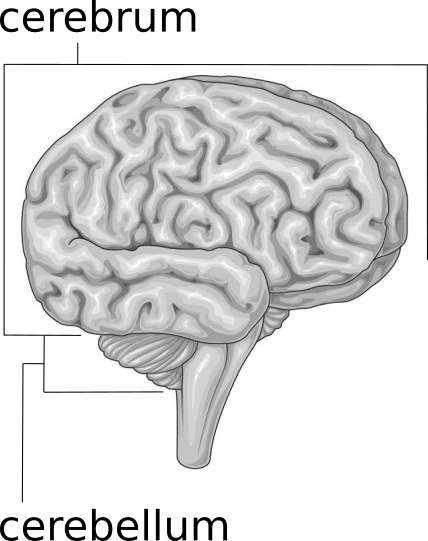
\includegraphics[width=\textwidth]{images/manually_created/brain/brain_cerebrum_cerebellum_text.png}
%   \end{center}
%   % https://smart.servier.com/smart_image/smart-brain-overview/
%   \caption[An artistic illustration showing cerebrum and cerebellum]{An artistic illustration showing cerebrum and cerebellum. Image adapted from Servier Medical Art, CC BY 4.0.}
%   \label{fig:brain_cerebrum_illustration}
% \end{subfigure}
% \begin{subfigure}{0.49\textwidth}
%   \begin{center}
%     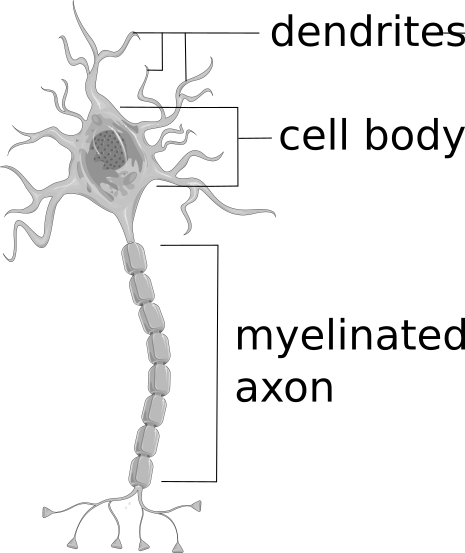
\includegraphics[width=\textwidth]{images/manually_created/brain/neurone_text.png}
%   \end{center}
%   % https://smart.servier.com/smart_image/smart-neuron-overview/
%   \caption[An artistic illustration of a neuron]{An artistic illustration of a neuron. The axon is myelinated (wrapped in fat); therefore, it is white, which gives a name to the white matter. Image adapted from Servier Medical Art, CC BY 4.0.}
%   %therefore, it is white. That is the reason, why is the white matter called white.
%   \label{fig:neuron_illustration}
% \end{subfigure}
% \end{figure}

\begin{figure}
  \begin{center}
    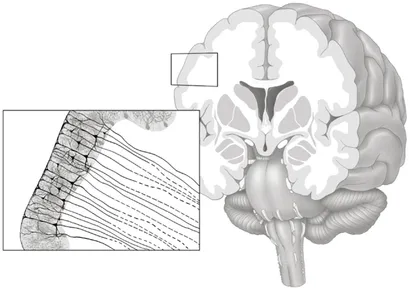
\includegraphics[width=\textwidth]{images/manually_created/brain/brain_matter_illustration.png}
  \end{center}
  \caption[An artistic illustration of gray and white matter]{The brain comprises gray matter in the outer layer and white matter in the inner layer. The lines in the zoomed-in diagram show axonal pathways leaving gray matter. An artistic illustration was created by Emma Vought, CC BY 4.0, and captions were added. \cite{bonilha_gray_2015}}
  \label{fig:brain_matter_illustration}
\end{figure}

\begin{figure}
  \begin{center}
    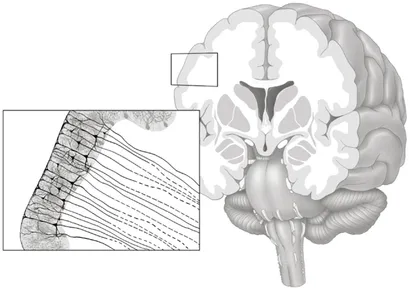
\includegraphics[width=\textwidth]{images/manually_created/brain/brain_matter_illustration.png}
  \end{center}
  \caption[An artistic illustration of gray and white matter]{The brain comprises gray matter in the outer layer and white matter in the inner layer. The lines in the zoomed-in diagram show axonal pathways leaving gray matter. An artistic illustration was created by Emma Vought, CC BY 4.0, and captions were added. \cite{bonilha_gray_2015}}
  \label{fig:brain_matter_illustration}
\end{figure}

\section{Magnetic Resonance Imaging}\label{sec:MRI}

Magnetic resonance imaging (MRI) is a widely employed technique that can be used to obtain a detailed picture of the brain. This section briefly introduces how MRI works. However, it is a simplification, and we recommend the book \textit{Magnetic Resonance Imaging: Theory and Practice} by Vlaardingerbroek and Boer for further information. \cite{vlaardingerbroek_magnetic_2003,bear_neuroscience_2016}

There is a great number of hydrogen atoms in the human body, both in water and fat. The protons in hydrogen nuclei have their own magnetic field because of the spin magnetic moment of the protons. When placed in a strong magnetic field in the MRI machine, some of the protons align themselves in parallel with the field. \cite{cizkova_comparing_2022}

When an electromagnetic pulse with the same frequency as the spinning protons (radiofrequency) is applied, the alignment is temporarily changed because the protons absorb the energy from the pulse and spin out of equilibrium. When the pulse is over, they return to their original alignment, emitting energy in the process. This energy is detected by a radio receiver. The MRI process consists of repeated cycles of the pulses.\cite{bear_neuroscience_2016,cizkova_comparing_2022}

In classical MRI, the fact that protons in different tissues and fluids change their magnetization differently causes different intensities of emitted energy and different brightness of the resulting image. Based on that, it is possible to distinguish different types of tissue. \cite{bear_neuroscience_2016,cizkova_comparing_2022}

\subsection{Diffusion weighted MRI}

What if we want to know not only that there is a white matter in a specific location but also the orientation of the axonal bundles connecting different areas of gray matter? This is when diffusion-weighted MRI (DW-MRI) is useful.

Diffusion is a process of transporting matter from one place to another by a random movement of molecules. The water in the brain (used in the MRI measurement as described above) also exhibits diffusion movement. Water diffuses much more easily along the axon membranes than across the axonal fibers. This fact is used to estimate the direction of axonal bundles by comparing the position of water molecules in subsequent MRI images. As a result, we obtain an estimation of axon fiber direction in each voxel in the resulting 3D image. \cite{bear_neuroscience_2016,jones_diffusion_2011,calamante_seven_2019}

For more details, we recommend a book \textit{Diffusion MRI: theory, methods, and applications} by D. K. Jones. \cite{jones_diffusion_2011}

\section{Electroencephalography}

In the previous section, we discussed MRI, which was used to measure the structural connectivity data in this thesis.\footnote{MRI could be used to measure function as well; so-called functional MRI is used, for example, for the reconstruction of resting state functional connectivity. However, we did not work with such data.} But how do we measure the function?

The communication and information processing in neurons is conducted via electrical signal transmission. The principle of electroencephalography (EEG) lies in measuring the difference in electrical potential caused by the brain activity between electrodes attached to the scalp. \cite{howseman_electroencephalographic_1999, st_louis_electroencephalography_2016, cooper_eeg_1974} We recommend a book \textit{EEG Technology} by Cooper, Osselton, and Shaw for more detailed information about EEG. \cite{cooper_eeg_1974}

The measurement has a temporal resolution in the range of milliseconds. Because of that, it is a suitable tool for recording the rapidly changing patterns of brain activity. However, it suffers from poor spatial resolution, which makes it difficult to infer the exact locations in the brain where the neural activity comes from. It is caused by the fact that the signal is a sum of activity generated by large groups of neurons under the electrodes weighted by the distance to the electrodes and the estimation of the signal sources is hard. \cite{howseman_electroencephalographic_1999, st_louis_electroencephalography_2016,michel_eeg_2019}

The EEG measurement results in one time series per electrode placed on the skull. However, what we truly want to know is the activation time series of specific locations inside the brain. We could perform source reconstruction to estimate the current sources that best fit the data to obtain activation time series per ROI instead of per electrode. See Figure \ref{fig:EEG} for illustration. The estimation process is complicated because the brain surface gray matter is folded, and the current spreads differently in different tissues in the brain. For an exact mathematical formulation of the source reconstruction problem and an overview of methods for solving the inverse problem, see \textit{Review on solving the inverse problem in EEG source analysis} by Grech et al. \cite{grech_review_2008}

\begin{figure}
  \begin{center}
    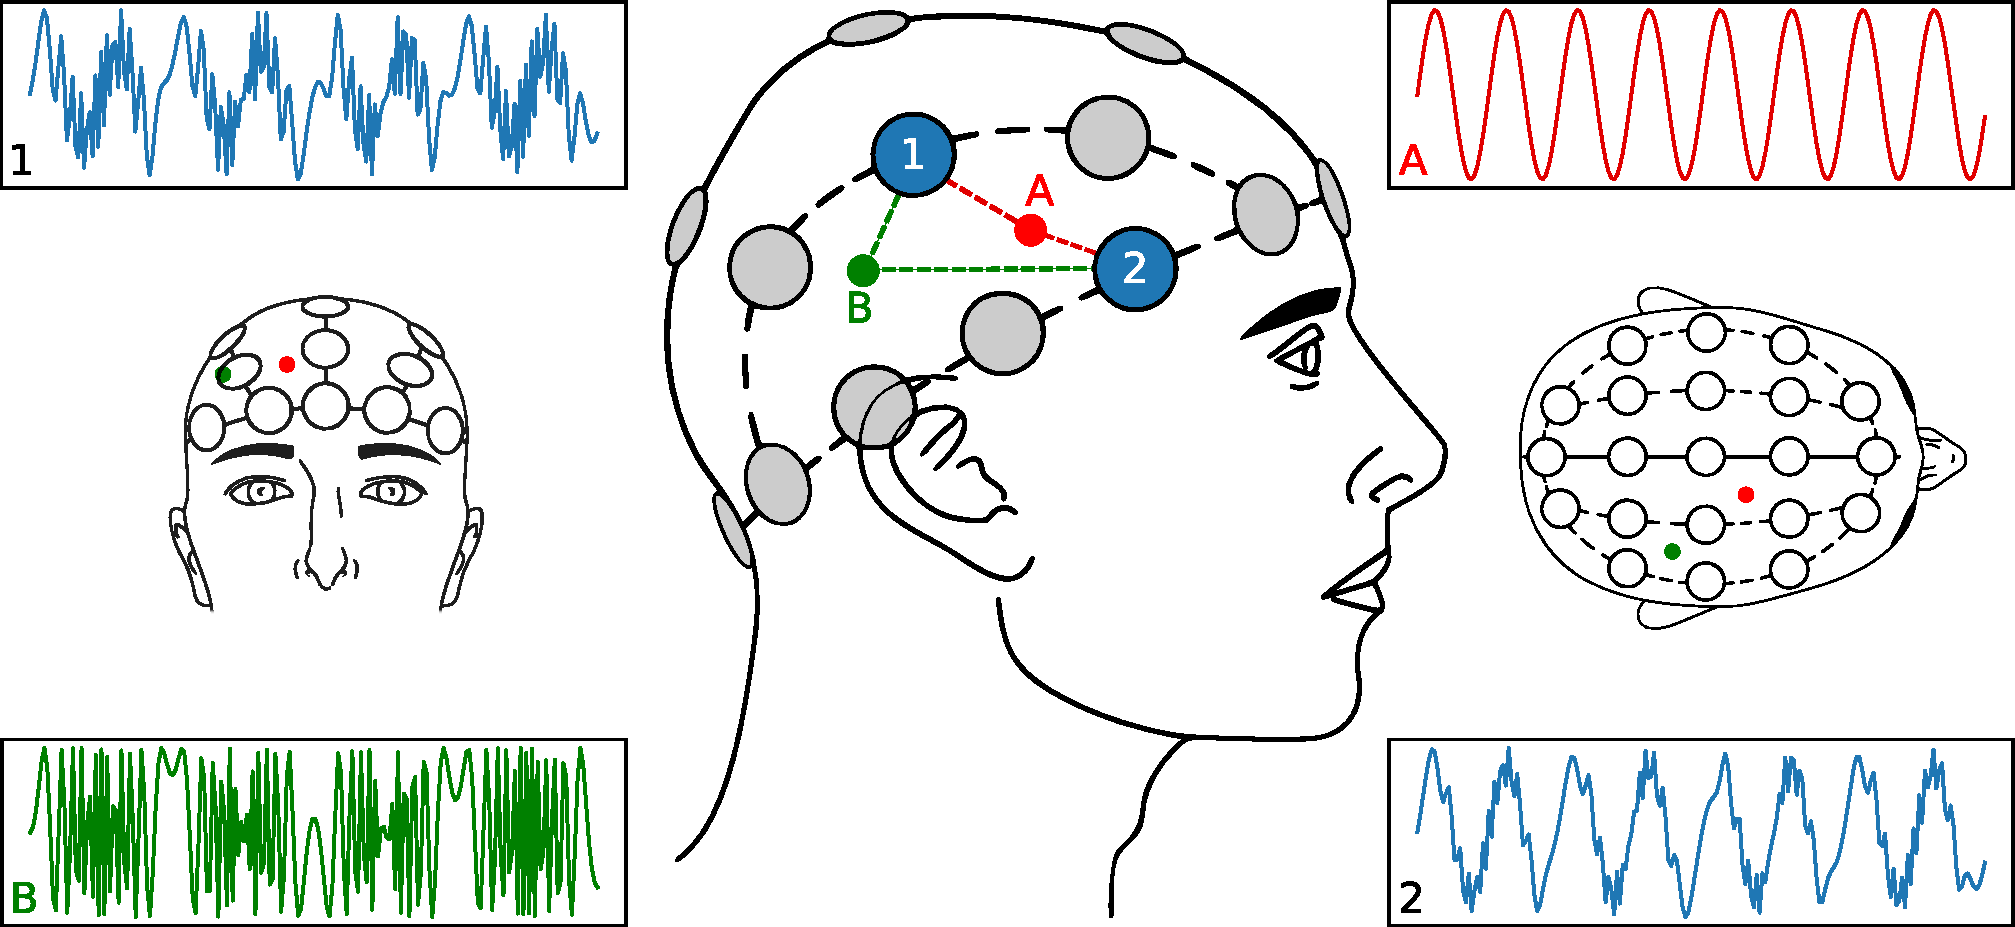
\includegraphics[width=\textwidth]{images/manually_created/brain/EEG_source_reconstruction.png.pdf}
  \end{center}
  \caption[An artistic illustration of EEG and its source reconstruction]{An illustration of EEG and its source reconstruction. Let us consider measurement sites 1 and 2 and their corresponding time series. The source reconstruction process aims to determine the activity at some places inside the skull, for example, A and B. Head and EEG montage images adapted from Servier Medical Art, CC BY 4.0.}
  \label{fig:EEG}
\end{figure}

\subsection{iEEG}\label{sec:iEEG}

Intracranial electroencephalography (iEEG) is an invasive measuring method; the electrodes are implanted into the skull. Because of that, the source reconstruction is not necessary. It has much better spatial resolution than the scalp EEG described above and also a high signal-to-noise ratio because it measures the neuronal responses around its origin. On top of that, it enables direct electrical stimulation of the brain by applying precise electric pulses to specific brain areas.
All of this makes iEEG one of the best methods to measure the dynamic changes of brain activity across time and space after a stimulation. However, due to ethical issues with implanting electrodes in the human brain, iEEG recordings are typically performed in drug-resistant epilepsy patients for clinical purposes, which makes iEEG less common than other noninvasive neuroimaging methods. In this thesis, we use data from the \textit{The Functional Brain Tractography project} (F-TRACT), which was also performed in epileptic patients. \cite{axmacher_what_2023,seguin_communication_2023}

\subsection{TMS-EEG}\label{sec:tms-eeg_measurement}

Transcranial magnetic stimulation EEG (TMS-EEG) is a noninvasive alternative to iEEG when we want to study the reaction of the brain to a stimulation. It combines scalp EEG measurement with TMS stimulation when applying magnetic pulses over the scalp triggers electrical activity in specific brain regions. The stimulation is produced by a brief electric current passing through a magnetic coil, which generates a brief magnetic field of high intensity. The magnetic field induces an electric field in the brain, and the voltage and induced currents excite the neurons in the area. \cite{hallett_transcranial_2007}




\chapter{Brain structural connectivity}\label{ch:SC}

The transfer of information and functional integration between different parts of the brain is facilitated by white matter connections. The nature of the dependency of brain function on its structure is not entirely clear and their relationship is still under active research. However, there is no doubt that the relationship exists. In this work, we focus on the relationship between brain function, specifically its reaction to a stimulus, to the structure. 

Mapping billions of individual neurons in the human brain is intractable. However, on the level of the whole brain, the structural connections can be assessed on the level of white matter pathways, which consist of nerve fiber bundles. Structural connectome is a simplified representation, which describes the structure of white matter fiber bundle pathways as a graph. Vertices represent parts of the brain, and edges represent their anatomical connections. The connectome is usually represented as a connectivity (adjacency) matrix. \cite{yeh_mapping_2021}

The first section of this chapter describes the process of obtaining structural connectome. The following section is devoted to the specific connectomes used in this work.

\section{Structural connectome acquisition}

Structural connectome construction aims to give a macroscopic view of the brain structure. The problem consists of two parts. First, we have to define how to divide continuous grey matter into areas forming nodes. Second, we must estimate the length and \enquote{strength} of the white matter fiber bundles connecting these nodes to add weighted edges to the graph.

There are various approaches how to obtain structural connectome, both invasive and non-invasive. In this work, we consider diffusion-weighted magnetic resonance imaging (DW-MRI) and tractography, which is a non-invasive approach. It is an indirect method (it does not explicitly measure the quantity of interest), and because of that, it suffers from several limitations, extensively described in a paper The Seven Deadly Sins of Measuring Brain Structural Connectivity Using Diffusion MRI Streamlines Fibre-Tracking by Calamante et al. \cite{calamante_seven_2019}. Because of that, it is error-prone, and the results should be treated with caution. \cite{sotiropoulos_building_2019}

\subsection{Node definition using brain parcellation}

As described in Section~\ref{sec:MRI}, the result of the MRI is a 3D image. The next step is dividing continuous grey matter, represented by voxels in the 3D image, into a bearable number of discrete nodes. The resulting division is called parcellation, and the parcels/nodes are called regions of interest (ROI). 

The simplest and most common approach how to obtain brain parcellation is using one of the so-called anatomical atlases. An anatomical parcellation atlas is a standardized map of the brain based on anatomical features such as neural macrostructures (for example, sulci and gyri -- depressions or furrows and ridges on the cerebral cortex). Atlas-based image recognition works as follows: For a sample patient image, objects in the image can be recognized by registration of the sample image with the atlas image. By aligning corresponding points between the sample and atlas images, the labels assigned to regions in the atlas image can be transferred and applied to the sample image. \cite{sotiropoulos_building_2019, lawrence_standardizing_2021,chang_ljchangdartbrains_2020,rohrer_focused_2008} 

There are various parcellation atlases stemming from various a\-na\-to\-mi\-cal or functional perspectives. Created through a range of techniques, these parcellations enable various insights into the brain organization and network properties. However, the use of different parcellations across studies brings difficulties when comparing different studies and complicates reproducibility. The parcellations vary not only in the number of nodes but also in their positions. Because of that, results may vary; while one parcellation may reveal a particular effect, it might not be observable with another parcellation (see Section \ref{sec:ftract_dkt}). \cite{sotiropoulos_building_2019, lawrence_standardizing_2021}

Lawrence et al. made an effort to standardize the human brain parcellations in the Neuroparc project available on GitHub\footnote{\url{https://github.com/neurodata/neuroparc}}. For a nice summarization of various approaches to brain parcellation and a list of parcellation atlases, let us also recommend \textit{Introduction to Parcellations}\footnote{\url{https://dartbrains.org/content/Parcellations.html}, accessed 1. 5. 2024} by Sava-Segal and Botch (part of an online coursebook DartBrains by Luke Chang). \cite{chang_ljchangdartbrains_2020}

\subsubsection{Selected parcellations}\label{sec:parcellations}

We came across several parcellations while working with structural connectivity matrices. We provide their list, including short descriptions. 

\begin{itemize}
    \item \textbf{Yeo}\label{parc:Yeo} \cite{thomas_yeo_organization_2011}: The parcellation is based on the main functional areas in the brain and it was created using data from 1000 healthy subjects using a clustering approach. It divides the brain into 7 or 17 functional areas based on the version. We use the 7 networks version to color nodes of Schaefer parcellation (below) based on their functionality, see Figure \ref{fig:schaefer_colored_by_yeo}.

    \item \textbf{Schaefer200}\label{parc:Schaefer200}  \cite{schaefer_local-global_2018}: The parcellation is based on functional data from task-based fMRI and resting-state fMRI. There are several versions based on the level of detail, the number of parcels could range from 100 up to 1000. We used a version with 200 parcels. Each parcel also comes with Yeo's 7 Networks label.
    There is a parcellation is available on GitHub.\footnote{\url{https://github.com/ThomasYeoLab/CBIG/tree/master/stable_projects/brain_parcellation/Schaefer2018_LocalGlobal}}
\end{itemize}

\begin{figure}[!h]
  \begin{center}
    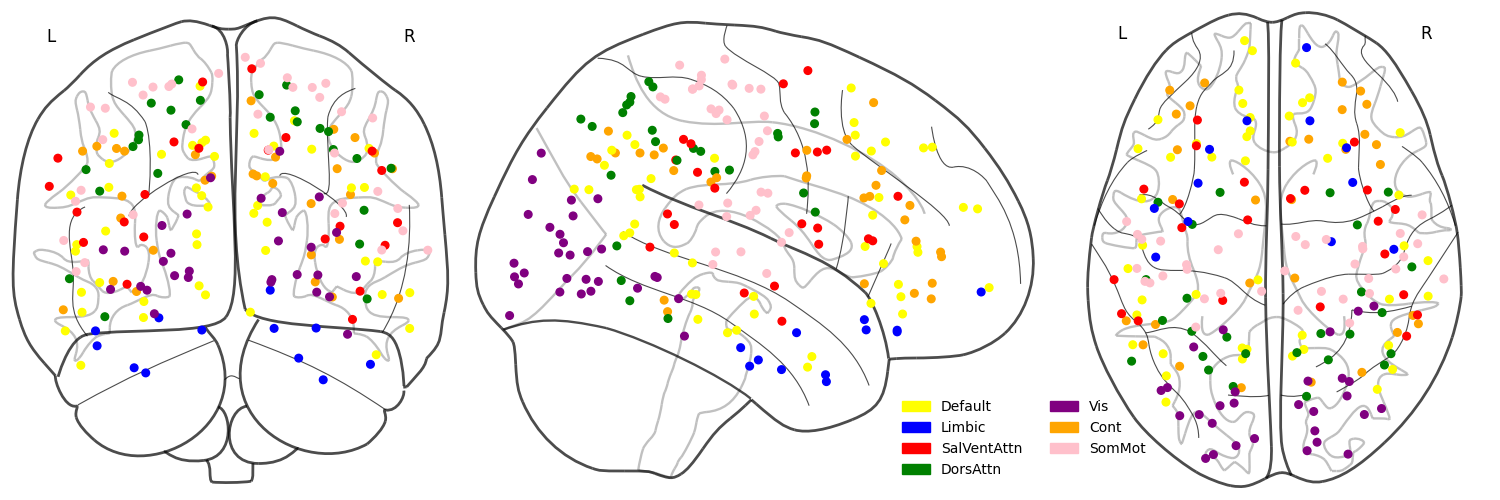
\includegraphics[width=\textwidth]{images/manually_created/Yeo7.png}
  \end{center}
  \caption[Schaefer200 centroids colored by Yeo7 networks]{Schaefer200 ROI centroids colored by Yeo7 networks.}
  \label{fig:schaefer_colored_by_yeo}
\end{figure}


\begin{itemize}
    \item \textbf{Desikan–Killiany (DK)}\label{parc:DK}  \cite{desikan_automated_2006}: The DK parcellation is defined by gyri. It was generated using 40 subjects (30 healthy and 10 with Alzheimer’s disease). It consists of 68 regions, 34 per hemisphere. There is also an updated Desikan-Killiany-Tourville (DKT) \cite{klein_101_2012} version of this parcellation, which merges regions that were not clearly defined. Because of that, DKT has only 62 regions. There is often confusion about which parcellation was used. We use only the version with 68 regions in this thesis, but the data sources sometimes mark it as DKT. Because of that, if the abbreviation DKT occurs, note that it also denotes Desikan–Killiany in our case.

    \item \textbf{Glasser}\label{parc:Glasser}  \cite{glasser_multi-modal_2016}: The parcellation is defined using a multimodal approach, combining brain anatomy (myelin content and cortical thickness), function (MRI measured during different tasks), connectivity (resting-state functional MRI) and topography. It is constructed based on data from 210 healthy subjects. It consists of 360 regions, 180 per hemisphere, which is the most detailed parcellation used in this work. It is sometimes denoted as MNI-HCP-MMP1.
\end{itemize}

In practice, we encountered several issues with parcellations usage. First of all, when we want to use a publicly available structural connectivity matrix, it is necessary to know not only which parcellation was used but also how the regions of interest are ordered in the matrix. Some authors use alphabetical ordering, while others use ordering based on the spatial proximity of the regions or their functional similarity. The main problem is that the paper does not always indicate the version. Therefore, we recommend being careful when using connectivity matrices from external resources.

Another problem was caused by the fact that the brain parcellation could use various coordinate systems.\footnote{Further information about coordinate spaces can be found in \textit{Coordinate Systems Appendix} of \textit{The Brain Imaging Data Structure} specification. The appendix is available on GitHub \url{https://github.com/bids-standard/bids-specification/blob/master/src/appendices/coordinate-systems.md} (accessed 1. 5. 2024). \cite{gorgolewski_brain_2016}} Because of that, it might be complicated to match data from two different resources even if they have the same parcellation.


\subsubsection{Node coordinates}

It is useful for the subsequent network analysis to keep the information about the spatial distances of the nodes. Because of that, we need to assign 3D coordinates to each node. The coordinates are obtained as a center of mass of the voxels registered as a part of the region of interest. They could be calculated for the atlas \enquote{model brain} or separately for each patient sample. For simplicity, we consider only the first option because we are working with average data, and the small differences are not of interest to us.

\subsection{Edges estimation}\label{sec:edge_estimation}

Conceptually, we want to create a map of long-range white matter fibers connecting the gray matter regions of interest discussed above. 

As explained in Section~\ref{sec:MRI}, DW-MRI measures water molecules' diffusion in brain tissues. It gives us information about the intravoxel axon arrangement. Based on this information (combined with some anatomical restrictions), a technique called tractography reconstructs the most probable streamline paths in white matter by tracing the water diffusion direction from voxel to voxel. \cite{yeh_mapping_2021,iturria-medina_characterizing_2007} 

The next step is defining a measure of connectivity between nodes. There are many options, such as the number, length, volume, or probability of streamlines between the corresponding nodes, but the mean value of a diffusion metric itself could also be used. \cite{yeh_mapping_2021} In this work, we use measures based on streamline counts and lengths because these were published by the authors of the connectivity matrices used here.

% https://commons.wikimedia.org/wiki/File:MRI_DWI_sequence_showing_restricted_diffusion_in_the_mesial_dorsal_thalami.jpg
% https://en.m.wikipedia.org/wiki/File:White_Matter_Connections_Obtained_with_MRI_Tractography.png


\chapter{Network communication models}\label{ch:networks}

To unveil the principles of communication and information processing in the brain is a primary goal of neuroscience. Network neuroscience views the brain as a complex network of anatomical connections. It uses tools rooted in graph theory to achieve this goal.  

Organization of connectomes follows numerous complex topological properties, such as modular and hierarchical structure or small-world\footnote{Small-world network combines high clustering (nodes tend to form densely connected clusters) and short characteristic path length (spatially distant nodes are, on average, connected via a small number of edges). \cite{seguin_brain_2023}} architecture. They are believed to evolve in support of efficient neural communication. \cite{seguin_brain_2023,avena-koenigsberger_communication_2018}

It is well-known that structural connections allow direct communication between neural elements. However, the communication between brain regions via indirect connections is not well understood. A growing number of communication models aim to provide insight into the communication process. The communication model is a theoretical framework used to understand how information flows within a network represented by a graph and is often represented using an algorithm that guides signals between network nodes. \cite{seguin_brain_2023}

Currently used communication models were greatly summarized by Seguin, Sporns, and Zalesky in the review article \textit{Brain network communication: concepts, models and applications} published in 2023. \cite{seguin_brain_2023} We present the main ideas of network communication models in this chapter. There are many communication models; we describe only the ones used in the rest of the thesis.

Our goal regarding the rest of the work is to use the structural connectome as a starting point for the calculation of matrices representing the speed level of information transfer between all pairs of nodes, assuming each of the communication models, i.e. how easy or fast it is to transfer the information between the nodes. We later investigate the correlation between those matrices and functional data. Hence we explain how to calculate the matrices for the selected communication models.

We used netneurotools, a package for Python, for the practical calculation of the matrices; all the communication models discussed below are implemented in the package.

\section{Decentralized vs centralized communication models}

The degree of centralization is an important feature of a network communication model. It refers to the extent to which the influence over communication flow is concentrated within some authority that knows about the whole network topology versus being distributed across the network. \cite{seguin_brain_2023}

What does it mean? The human brain is believed to be a decentralized system in which individual elements such as neurons probably do not have complete information about the whole brain network in which they are embedded. \cite{seguin_brain_2023} From another point of view, brain organization and communication evolved to minimize the metabolical cost. \cite{bullmore_economy_2012} As stated in a paper by Avena-Koenigsberger et al. from 2018 \cite{avena-koenigsberger_communication_2018}, p. 19:
\begin{quote}
The shortest path length is thought to be an indicator of the ease with which signals can be transmitted between two nodes. In neural systems that communicate via electrochemical transmission, minimizing the number of synapses between any two neuronal elements (that is, path length) is intuitively desirable. Longer paths are more susceptible to noise, are more likely to involve a greater number of distinct processing steps, incur longer transmission delays, and are energetically (metabolically) more expensive to construct and use.
\end{quote}
However, to send the information via the shortest path, the neurons should have information about their surroundings and the path lengths in the brain. The question is, how much do the neurons \uv{know} what path is the shortest one? And generally, do centralized models better explain communication within the brain than decentralized ones?

\section{Diffusion processes}

Diffusion processes build on the idea that individual nodes do not have knowledge about the overall network architecture. They propose a concept of signal propagation via broadcasting and random walks. Therefore, the signal transmission requires more signal forwarding to send messages between two nodes, and thus, it might suffer from higher delays and higher energetic (metabolic) costs. \cite{seguin_brain_2023}

\subsection{Diffusion efficiency (DIF)}

Diffusion efficiency assumes that information in the brain is distributed via unbiased random walks. The signal under this assumption travels from node $i$ randomly to one of its neighbors $j$ with probability proportional to the weight of edge to $j$. The transmission continues following this rule until the target node is reached. \cite{seguin_communication_2023,seguin_brain_2023}

Formally, the probability of transmission from $i$ to $j$ in one step is given by transition probability matrix $T$ defined as follows 
$$
T_{ij} = \frac{W_{ij}}{\sum_{n=1}^N W_{in}}
$$
where $W$ is the matrix of structural connectivity weights, and $N$ is the number of nodes. We can analytically compute the average number of steps needed by a random walker to get from $i$ to $j$ using the matrix $T$. Let us denote this average number of steps as $H_{ij}$. Diffusion efficiency matrix $DIF$ is then computed as 
$$
DIF_{ij}=1/H_{ij}.
$$

\subsection{Communicability (COM)}

Communicability is a communication model based on broadcasting. That means we do not assume signal propagation from a node $i$ to a node $j$, but simultaneously to many other nodes in each step. Communicability assumes that each node always propagates the signal to all its neighbors. It does not matter if some of the neighbors already received the signal earlier. \cite{seguin_communication_2023,seguin_brain_2023}

We use the formal definition of communicability in weighted networks by Crofts and Higham \cite{crofts_weighted_2009}. Let $W$ be the matrix of weights. Let us define the generalized degree of a node $i$ as $d_i = \sum_{k=1}^N W_{ik}$ where $N$ is the total number of nodes. The normalized matrix $W'$ is then defined as 
$$
W'_{ij} = \frac{W_{ij}}{\sqrt{d_i}\sqrt{d_j}}
$$
The communicability $COM$ between two nodes $i$ and $j$ is then defined as
$$
COM_{ij} = e^{W'_{ij}}.
$$

Concluding remark to communicability, according to a paper by Seguin et al. from 2023 \cite{seguin_brain_2023}, p. 563:
\begin{quote}
Communicability is a popular measure in network neuroscience, constituting one of the most commonly adopted alternatives to shortest-path measures.
\end{quote}

\subsection{Search information (SI)}

Search information is based on the notion of random walks. It quantifies the amount of information, measured in information bits, needed to bias the random walker representing the signal in the network to take the shortest path between two nodes. The model relates to the accessibility of short and efficient paths under the assumption of the diffusive communication model. \cite{seguin_communication_2023,seguin_brain_2023}

How does it work? Let us assume that the information needs to be transferred from node $i$ to node $j$ through the shortest path, expecting that if there are more shortest paths, any of them could be selected. It is necessary to know which edge to take in each node along the path. Without any prior knowledge, the information needed to select an exit from a node with $k$ unweighted adjacent edges is $\log_2(k)$. \cite{rosvall_searchability_2005,rosvall_networks_2005}

For each path $p(i,j)$ from $i$ to $j$, the probability that the random walker follows this path is 
$$
P[p(i,j)] = \frac{1}{k_i}\prod_{v \in p(i,j)}\frac{1}{k_v-1}.
$$
where $k_i$ is a degree of node $i$. There is $k_v-1$ instead of $k_v$ because we know which path was taken on the way to $j$. Therefore, we can reduce the number of possible exit edges by one. As a result, the probability of getting from node $i$ to node $j$ using any of the shortest paths is 
$$
P_{ij} = \sum_{\{p(i,j)\}}P[p(i,j)] 
$$
where $\{p(i,j)\}$ is a set of all shortest paths connecting $i$ and $j$. Using this, we can define the search information matrix $SI$ as 
$$
SI_{ij}=-\log_2 P_{ij}.
$$

This could be explained as \uv{the total information value of knowing any of the shortest paths between $i$ and $j$}. For the weighted case, we can just replace the probability $1/(k_i-1)$ of taking a specific exit from node $i$ by $w_e/(w_i-w_{in})$ where $w_e$ is the weight of the specific edge, $w_i$ is the sum of weights of all edges adjacent to $i$ and $w_{in}$ is the weight of the edge taken when arriving to the node. 

\section{Routing protocols}

Routing protocols are grounded in the idea that messages are routed through the network using single, selectively accessed paths. It builds up on the fact that the transmission of information is costly, and thus, the brain evolved to optimize it. The most widely used communication model in brain networks, shortest path routing, belongs to this group. \cite{seguin_brain_2023}

However, knowledge about network topology is highly unlikely in real neural systems. Besides, if the communication relies exclusively on the shortest paths, it excludes near-optimal alternatives. \cite{avena-koenigsberger_communication_2018}

\subsection{Shortest path efficiency (SPE)}

According to Seguin et al. \cite{seguin_brain_2023}, the shortest path routing model is the most common and widely used in network neuroscience. The key assumption of this model is that the signals in the brain follow the shortest paths because it is the most efficient option.

The calculation of shortest path efficiency is pretty straightforward. First, the shortest paths are calculated between all node pairs $\Lambda^*_{ij}$. The shortest path efficiency $SPE$ is then defined as 
$$
SPE_{ij}=\frac{1}{\Lambda^*_{ij}}.
$$

\subsection{Navigation efficiency (NAV)}

Navigation routing protocol uses a greedy strategy to transmit the signal \uv{in the right direction} based on the spatial distribution of the nodes. Let us assume the signal travels from node $i$ to $j$. For each node along the way starting from $i$, we identify its neighbor with the smallest Euclidean distance to $j$, and progress to it. The process is repeated until $j$ is reached and we sum the lengths of edges along the path, denoting the sum $\Lambda_{ij}$. Then, same as for the shortest path efficiency, navigation efficiency is defined as 
$$
NAV_{ij}=\frac{1}{\Lambda_{ij}}.
$$

Note that this protocol uses structural connectivity only to get the connectedness of the graph and the navigation is based on Euclidean distance. The length of edges of the structural connectome is only used at the end to get the real length of the path.

\section{Parametric models}

Concerning the degree of centralization, parametric models lie between routing protocols and diffusion processes. Their crucial characteristic is the presence of a tunable parameter. Depending on its value, the model can act as a routing protocol, diffusion process, or something between these two extremes. \cite{seguin_brain_2023}

An example of a parametric model is a biased random walk model, where the random walker is biased by some topological properties of the network or domain-specific properties of the nodes. This could be implemented in the structural connectivity network of the brain as a parameter enabling the individual nodes to \uv{know} more and more about their neighborhood and utilize this knowledge to navigate the random walker. \cite{seguin_brain_2023}

We did not use any parameter model in this work because they require careful parameter tuning, and we wanted to try more different models to obtain a broad picture rather than closely examine the parameters of one parametric model. This might be an interesting direction for future research.

\chapter{F-Tract}\label{ch:ftract}

The entry point of this thesis is the paper \textit{Communication dynamics in the human connectome shape the cortex-wide propagation of direct electrical stimulation} by Sequin et al., published in 2022. It shows that the network communication models discussed in Chapter \ref{ch:networks} computed using structural connectome based on DW-MRI can, up to some degree, explain the propagation of focal electrical stimulation through the brain. 

The main question of this thesis is whether it is possible to apply the methodology used by Seguin et al. to find correlations between the response to an intracranial stimulation and network communication models to TMS-EEG data. Before diving into that, let us devote this chapter to a closer investigation of the aforementioned paper and our experiments with the Functional Brain Tractography project (F-TRACT) iEEG functional data.  

\section{F-TRACT iEEG functional data}

The Functional Brain Tractography project (F-TRACT)\footnote{\url{https://f-tract.eu/}} summary dataset used in this section was prepared by Jedynak et el. \cite{jedynak_f-tract_2023} and it is available from the EBRAINS platform.\footnote{\url{https://doi.org/10.25493/H0JJ-0YD}} It consists of several matrices characterizing the brain's response to intracranial electrical stimulation.

The F-TRACT project aggregated iEEG data from 550 patients with drug-resistant epilepsy measured during $29\,055$ stimulations using 2.77 million pairs of intracerebral depth electrodes. In order to mitigate the impact of epileptogenic processes in further analyses, recordings with a high likelihood of pathological activity were excluded. The results were projected onto a number of parcellations. We use Glasser parcellation in this chapter (more in Section \ref{sec:parcellations}). \cite{jedynak_f-tract_2023,seguin_communication_2023} 

The recorded evoked potentials were baseline corrected\footnote{Baseline correction is based on utilizing EEG activity from a baseline period—before an external event—to adjust activity during a post-stimulus interval.} and $z$-scored. Stimulus response was considered significant if the $z$-scored evoked potential over $z = 5$ was observed. The response amplitude was defined as the first peak of $z$-scored evoked potential above the $z = 5$ threshold. Using that, two whole-brain group-level matrices were constructed. Entries $P_{ij} \in [0,1]$ of response probability matrix $P$ characterize the probability that we observe a significant response as described above in ROI $j$ after stimulation of $i$. Entries $A_{ij} \in \mathbb{R}_{>0}$ of response amplitude matrix $A$ capture the median response amplitude of significant responses.

It is important to mention that the dataset available on EBRAINS publishes the response probability and amplitude matrices in two versions, one considering responses up to 50 ms after the stimulus and the other up to 200 ms after the stimulus. However, Sequin et al. used the responses up to 800 ms after the stimulation.\footnote{They used the 200 ms version in robustness analysis, it can be found in the Supplementary information of the paper. \cite{seguin_communication_2023} } That might be a source of discrepancy in the results.

\section{Results}\label{sec:ftract_results}

In this section, we present the results of our replication of the work by Sequin et al. \cite{seguin_communication_2023}. There is a key difference between our results and the original paper in that we used not only structural connectivity weights derived from streamline counts between individual ROI, but also streamline lengths. We show that the lengths correlate very well with the response probability.

We used several structural connectivity matrices obtained from several datasets. More about the construction of these specific matrices and experiments with them can be found in Chapter \ref{ch:SC_indepth}. All the matrices were pruned to keep graph density $25\%$.

For each dataset, we calculated the communication metrics matrices described in Chapter \ref{ch:networks}. Table \ref{tab:matrices_usage} shows which matrices were used as inputs for the metrics. It is an important comparison because we want to know if the communication metrics bring any advantage over plain structural connectivity or Euclidean distances, i.e. do we get anything new by using communication metrics with these inputs over the inputs themselves? 

\begin{table}
    \centering
    \begin{tabular}{l| l}
        metric & matrices  \\
        \hline
        $SPE$   & $SC_L$ \\
        $SPE_W$ & $1/SC_W$ instead of $SC_L$ \\
        $COM$   & $SC_W$ \\
        $SI$    & $SC_W$ for navigation, $ED$ for path length \\
        $SI_L$  & $SC_W$ for navigation, $SC_L$ for path length \\
        $NAV$   & $SC_W$ only to get connectedness, $ED$ ($SC_L$ for path length) \\ 
        $DIF$   & $SC_W$ \\
    \end{tabular}
    \caption[Matrices used in communication metrics calculation]{Matrices used in communication metrics calculation, $SC_W$ structural connectivity weights, $SC_L$ structural connectivity lengths, $ED$ Euclidean distances. For navigation efficiency ($NAV$) we used $SC_L$ for path length calculation if available, otherwise $ED$.}
    \label{tab:matrices_usage}
\end{table}

We used the Spearman correlation coefficient of the response matrix and structural and communication matrices to evaluate the relationship between structure and function. It is a reasonable choice because we want to see if the response probability is higher in regions that are \uv{easier to access}, but we do not expect the relationship to be linear, thus we do not use the Pearson correlation coefficient. Seguin et al. used Spearman correlation as well, so the results are comparable.

We always calculated full and partial correlation, the latter with the influence of Euclidean distance controlled. The idea behind the partial correlation calculation is that we want to investigate how much of the response variance could be explained that was not accounted for by spatial proximity.

All the correlations were calculated for all ROI pairs (i. e. the whole matrix) where the response probability/amplitude was not nan (enough stimulations, enough significant responses, not too close, if close pairs excluded).

\subsection{Robustenss in structural connectome selection}\label{sec:sc-robustness_ftract}

First of all, the correlations are robust to structural connectome selection. Figure \ref{fig:ftract_alldata_long_probabilities} shows the correlations of response probabilities with structural matrices and communication metrics. Figure \ref{fig:ftract_alldata_long_amplitudes} shows the same for response amplitudes. We can see that there are differences in results based on the dataset and group-averaging method selection, but there are significant correlations for all of them and differences are generally rather small for most of the communication metrics.\footnote{Change of response length (50 ms, 200 ms) or excluding close pairs or regions do not reveal any new information.} Because of that, we present the rest of the results with only the Mica-Mics dataset and Rosen and Halgren's group averaging method for simplicity. \TODO[kde se dá kouknout na další výsledky]

We chose the Mica-Mics dataset because it provides Schaefer200 parcellation as well, so we can use the same dataset here and in the experiments with TMS-EEG data (Chapter \ref{ch:pytepfit}). The Rosen and Halgren's group averaging method is selected because it seems that it sometimes (e. g. $SC_W$ and $SPE_W$ in Figure \ref{fig:ftract_alldata_long_amplitudes}) results in higher correlations than the other approaches.

\begin{figure}
    \centering
    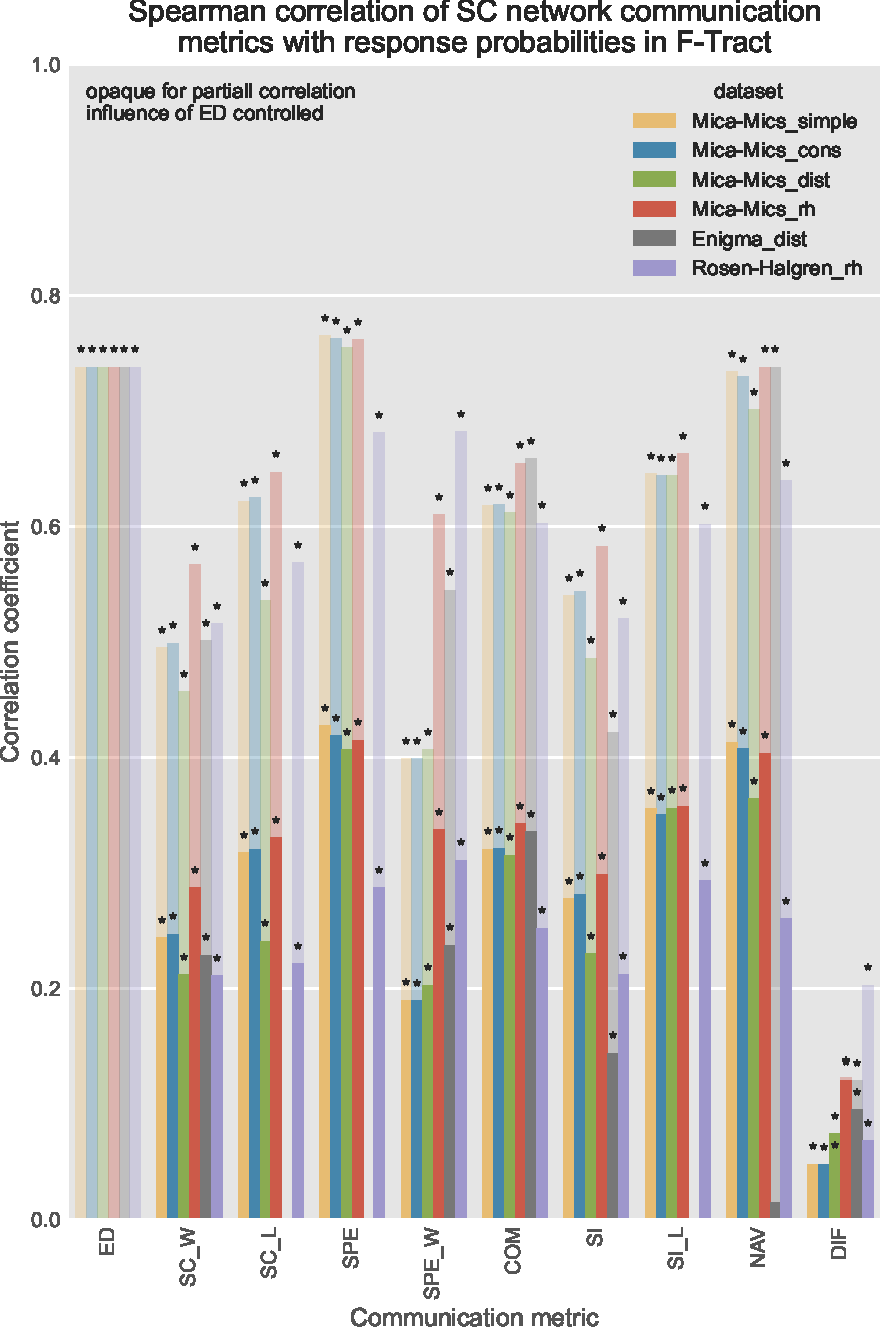
\includegraphics[width=0.93\textwidth]{images/nootebook_generated/ftract_results/MNI-HCP-MMP1/5/ED0/0.25/long/Spearman_correlation_of_SC_network_communication_metrics_with_response_probabilities_in_F-Tract.pdf}
    \caption[F-TRACT probability correlations - all $SC$ matrices]{Correlations (absolute value) of response probability (200~ms response) and structural connectivity and derived communication metrics. Asterisks denote a significant correlation ($p<0.05$).}
    \label{fig:ftract_alldata_long_probabilities}
\end{figure}


\begin{figure}
    \centering
    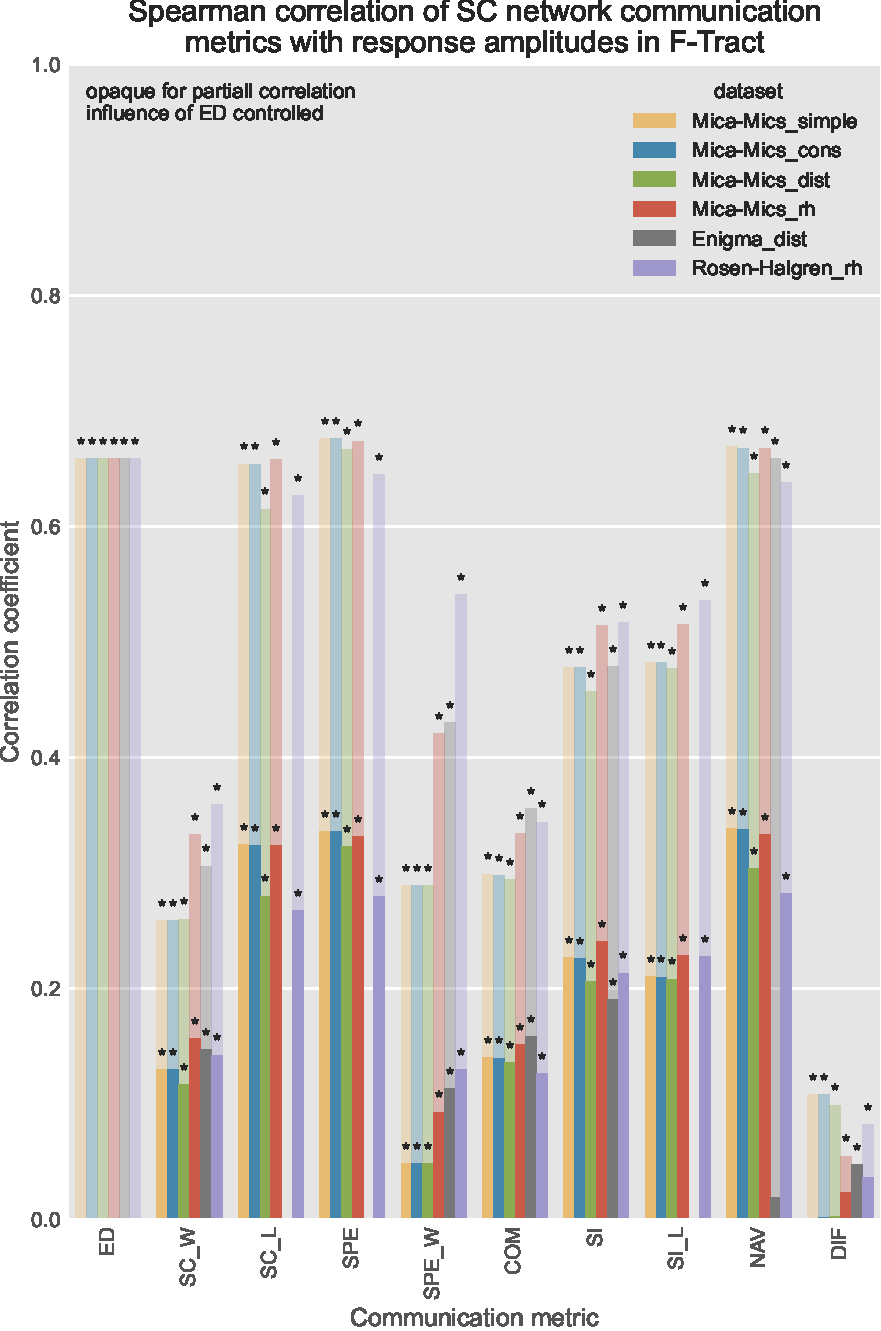
\includegraphics[width=0.93\textwidth]{images/nootebook_generated/ftract_results/MNI-HCP-MMP1/5/ED0/0.25/long/Spearman_correlation_of_SC_network_communication_metrics_with_response_amplitudes_in_F-Tract.pdf}
    \caption[F-TRACT amplitude correlations - all $SC$ matrices]{Correlations (absolute value) of response amplitude (200~ms response) and structural connectivity and derived communication metrics. Asterisks denote a significant correlation ($p<0.05$).}
    \label{fig:ftract_alldata_long_amplitudes}
\end{figure}


\subsection{Response vs communication metrics}

Could communication metrics be used to explain the response probability and amplitude of reaction on stimulus in individual ROIs? That was the main question of Seguin et al. \cite{seguin_communication_2023} and it is the focus of this thesis. We overall confirmed the results of Seguin et al. that there are correlations between the communication metrics and response probability and amplitude, and that those can overcome the correlations with the plain weights of the structural connectome. 

However, Seguin et al. did not use structural connectivity lengths, which appear to be correlated with both response probability (see Figure \ref{fig:ftract_alldata_long_probabilities}, column $SC_L$) and response amplitude (see Figure \ref{fig:ftract_alldata_long_amplitudes}, column $SC_L$) even better than the structural connectivity weights. It is a contribution of our work that we included structural connectivity lengths in the analysis. 

Let us look closer at the correlations for response probability and amplitude in the following subsections.

\subsubsection{Response probability}\label{sec:probability_F-Tract}

Seguin et al. showed a correlation of response probability with Euclidean distance of approximately $0.6$. Figure \ref{fig:ftract_alldata_long_probabilities} shows that we found an even higher correlation. This might be caused by the fact that Seguin et al. excluded pairs of ROIs that are closer than 20 mm from the analysis. They also considered the responses up to 800 ms after the stimulation. The Supplementary material of their paper shows the results without the close pairs exclusion and with 200 ms responses; both are closer to ours. Therefore we think that these factors may be a cause of overall higher correlations in our results. We also tried to exclude the close pairs (\TODO[kde to najít]), the correlations were generally slightly lower in that case. 

It can be seen in Figure \ref{fig:ftract_alldata_long_probabilities} that there are correlations between the response probability and structural connectivity and communication metrics. However, it is not possible to order all the metrics from the best to the worst one because of the differences in the input matrices (they differ in dataset and group-averaging method). Despite that, let us describe the main findings.

The shortest path efficiency $SPE$ calculated using the structural connectivity lengths yields the highest correlations with response probability across all parameter settings we tried. The correlation is consistently $>0.6$ (often $>0.7$) for both 50 ms and 200 ms responses, various datasets and it stays high if we exclude close pairs or ROIs from the analysis.

Another metric with a consistently high correlation with response probability is the navigation efficiency $NAV$ based on the idea of signal navigation in each node to the neighbor with the shortest Euclidean distance to the target. The length of the final path was calculated using structural connectivity lengths, which might be the reason for its similarity to the shortest path efficiency.

The third metric we want to discuss is communicability $COM$. It does not result in absolute correlations as high as the shortest path efficiency $SPE$ and the navigation efficiency $NAV$, but it is better than the structural connectivity weights that are the only input of this metric. 

Our results also agree with Seguin et al. that the diffusion efficiency $DIF$ is not useful for the characterization of the response probability because of low and often non-significant correlations. 

\subsubsection{Response amplitude}

First of all, the response amplitude matrix is sparser than the response probability matrix because amplitudes were included in the analysis only for regions with at least 100 significant responses. That may be a source of uncertainty in the response amplitude analysis. 

An interesting observation is that the structural connectivity lengths correlate with the amplitude much better than the structural connectivity weights and the difference is higher than for the response probability discussed in the previous section.

Generally, the response amplitudes correlate less with all the communication matrices. We do not discuss amplitudes closer in this section because, as shown in Chapter \ref{ch:pytepfit}, they are not useful in the generalization of the approach to TMS-EEG.

\subsection{Short (50 ms) vs long (200 ms) responses}\label{sec:response-length_F-Tract}

The investigation of the influence of the response length is important for the application of this approach to the TMS-EEG data. The TMS coil makes a sound when turned on, so the later responses in TMS-EEG data include the reaction of the brain to the auditory stimulus. 

Comparing Figure \ref{fig:ftract_mica_short_probabilities} and Figure \ref{fig:ftract_mica_long_probabilities} the structural connectivity and communication matrices show very similar full correlation for both 50 and 200 ms responses. We can see that the shorter responses correlate more with Euclidean distance and the partial correlations with Euclidean distance control are lower. According to the results, it seems that the earlier responses are driven more by Euclidean distance, while the later responses exhibit more complex behavior. 

\begin{figure}
    \centering
    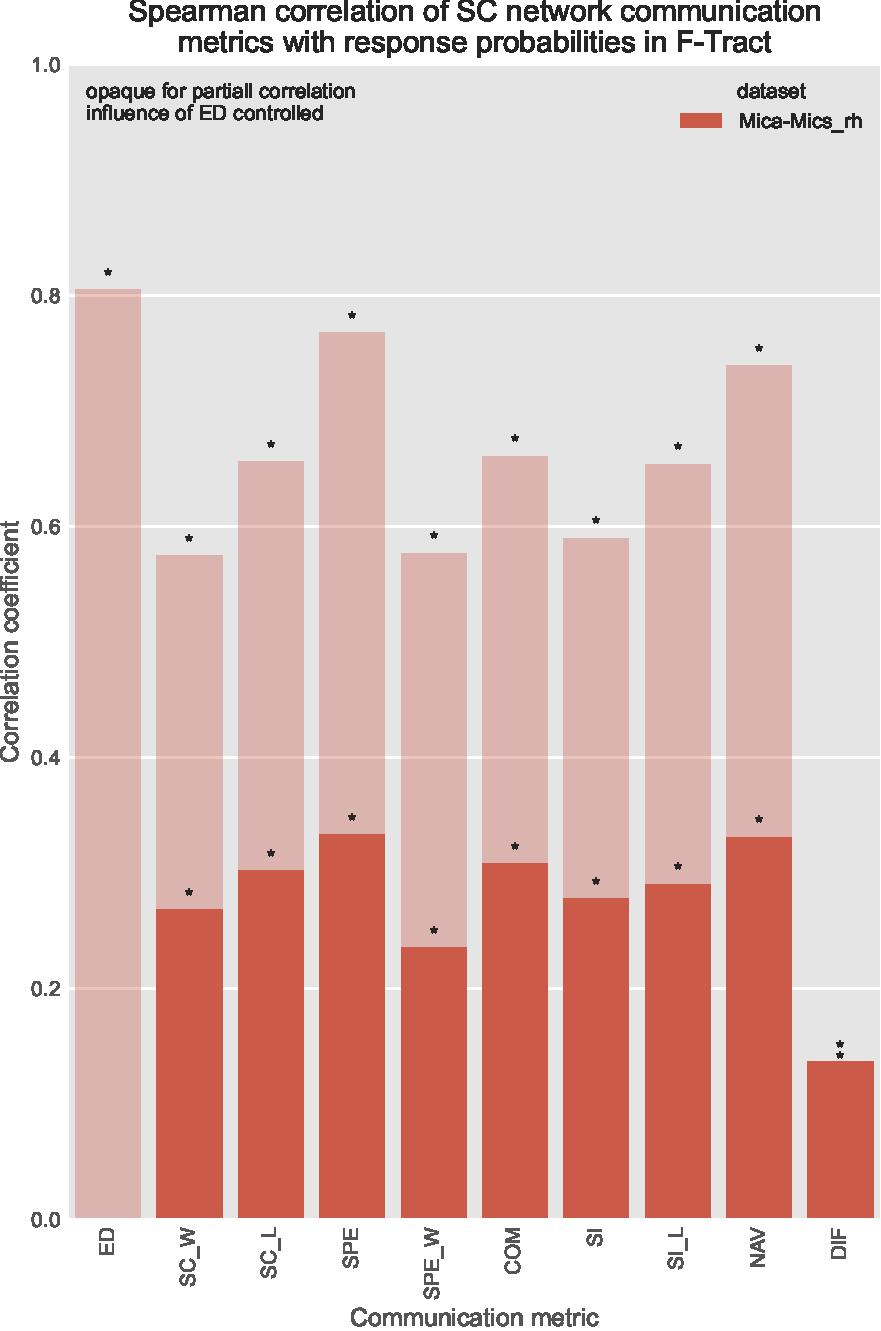
\includegraphics[width=0.93\textwidth]{images/nootebook_generated/ftract_results/MNI-HCP-MMP1/5/ED0/0.25/short/mica_rhSpearman_correlation_of_SC_network_communication_metrics_with_response_probabilities_in_F-Tract.pdf}
    \caption[F-TRACT probability correlations - Mica-Mics\_rh 50 ms]{Correlations (absolute value) of response probability (50~ms response) and structural connectivity and derived communication metrics. Asterisks denote a significant correlation ($p<0.05$).}
    \label{fig:ftract_mica_short_probabilities}
\end{figure}

\begin{figure}
    \centering
    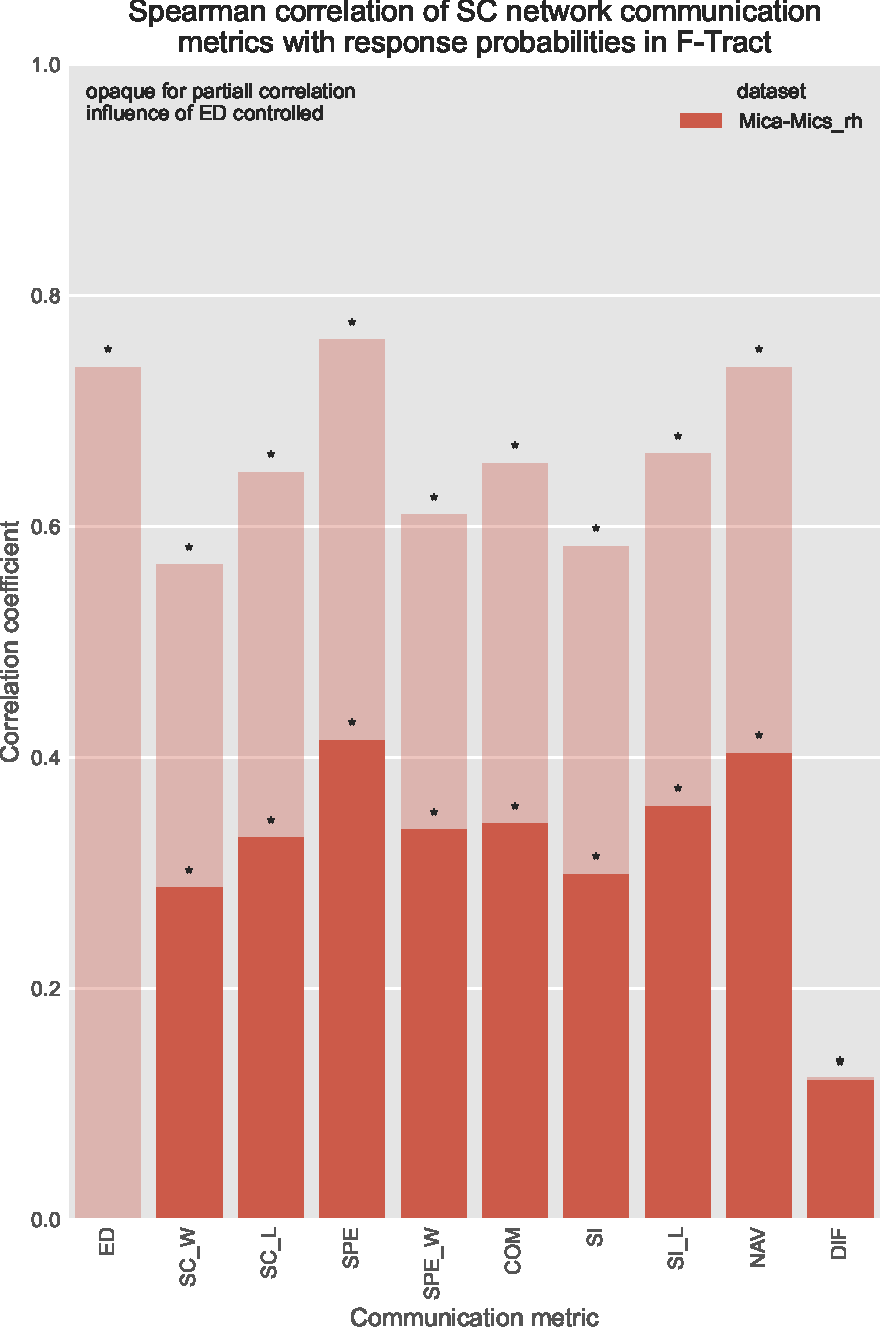
\includegraphics[width=0.93\textwidth]{images/nootebook_generated/ftract_results/MNI-HCP-MMP1/5/ED0/0.25/long/mica_rhSpearman_correlation_of_SC_network_communication_metrics_with_response_probabilities_in_F-Tract.pdf}
    \caption[F-TRACT probability correlations - Mica-Mics\_rh 200 ms]{Correlations (absolute value) of response probability (200~ms response) and structural connectivity and derived communication metrics. Asterisks denote a significant correlation ($p<0.05$).}
    \label{fig:ftract_mica_long_probabilities}
\end{figure}

\subsection{Response onset and peak delay}

Section \ref{sec:reponse_definition} discusses several options of \uv{response significance/strength} definition for TMS-EEG data. We confirmed Sequin et al.'s results showing a correlation between response probability and amplitude and the structural connectivity and communication metrics derived from it. However, the F-TRACT dataset also provides other characteristics of the responses, including response onset delay and response peak delay. Could those be used for response characterization and predicted using structural connectivity? We ran the analysis for them as well.

The partial correlations controlling for Euclidean distance are generally lower than $0.1$ and often not significant. For the 50 ms responses, the full correlations are generally lower than $0.2$, which we interpret as no relationship between the peak onset/delay and communication metrics in this case. However, the full correlations for 200 ms responses are significant and higher than $0.2$ for all communication metrics except the diffusion efficiency. For Euclidean distance, the correlation is $>0.4$ for both peak onset and delay. That suggests that there might be some relationship for longer responses and supports our idea of response characterization by its peaks in Section \ref{sec:reponse_definition}.

\subsection{Connected and unconnected regions}

The paper by Seguin et al. \cite{seguin_communication_2023} analyses the results not only for all region pairs, but also for connected and unconnected regions separately. We do not include this analysis because our main goal is an application of the approach to TMS-EEG datasets, for which it is not reasonable because we consider stimulation of a single site (not many different sites across the brain as here), so we have much less data.

\section{Results for primary motor cortex (M1) ROI}\label{sec:ftract_results_per_roi}

All the results presented above calculated the correlations for all ROI pairs together, expecting the stimulation of various ROIs. However, the TMS-EEG data we use in this thesis were measured during the stimulation of a single ROI, namely the left hemisphere's primary motor cortex (denoted M1), as stated in the data-describing paper from Biabani et al. \cite{biabani_characterizing_2019} Primary motor cortex in the left hemisphere is denoted L\_4 in Glasser parcellation. On the grounds of that, we selected only the row corresponding to L\_4 stimulation from the response probability matrix and the corresponding rows from the structural and communication matrices, and we calculated the correlations between these rows. 

Figure \ref{fig:ftract_mica_long_probabilities_L4} shows the results for the stimulation of M1 in the left hemisphere and 200 ms response. The results for the 50 ms response are very similar. Both show most of the full correlations above $0.6$ and partial correlations above $0.2$, with the shortest path efficiency $SPE$ having the highest full correlation with the response probability. Considering the partial correlations, the highest correlation is achieved with structural connectivity lengths $SC_L$.

\begin{figure}
    \centering
    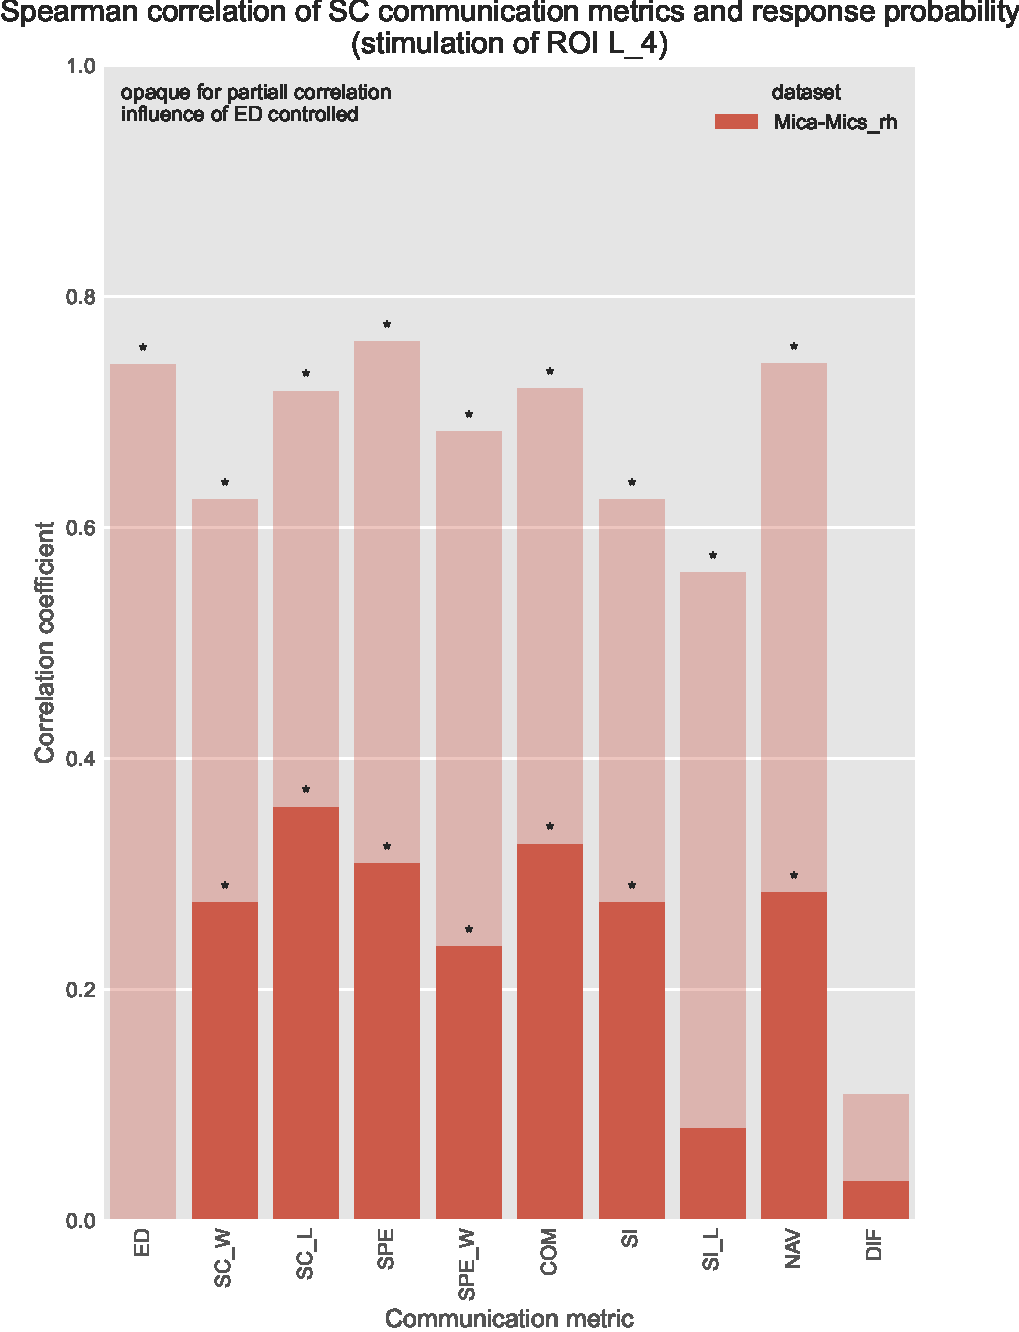
\includegraphics[width=\textwidth]{images/nootebook_generated/ftract_results_per_roi/long/MNI-HCP-MMP1/ED0/0.25/Spearman_correlation_of_SC_communication_metrics_and_response_probability_(stimulation_of_ROI_L_4).pdf}
    \caption[F-TRACT probability correlations - Mica-Mics\_rh L\_4]{Correlations (absolute value) of response probability (200~ms response) and structural connectivity and derived communication metrics. Asterisks denote a significant correlation ($p<0.05$).}
    \label{fig:ftract_mica_long_probabilities_L4}
\end{figure}

\subsection{Was the stimulation target really M1?}

Even though Biabani et al. \cite{biabani_characterizing_2019} declare they stimulated the primary motor cortex, the source-reconstruction of the TMS-EEG data by Momi et al. \cite{momi_tms-evoked_2023} suggest the stimulation of slightly different site, specifically L\_3b. This is further explained in Section \ref{sec:parcellations-mapping-stimulated_roi}. Here we just present the results for L\_3b stimulation in Figure \ref{fig:ftract_mica_long_probabilities_L3b}, so we can later use them for comparison.

\begin{figure}
    \centering
    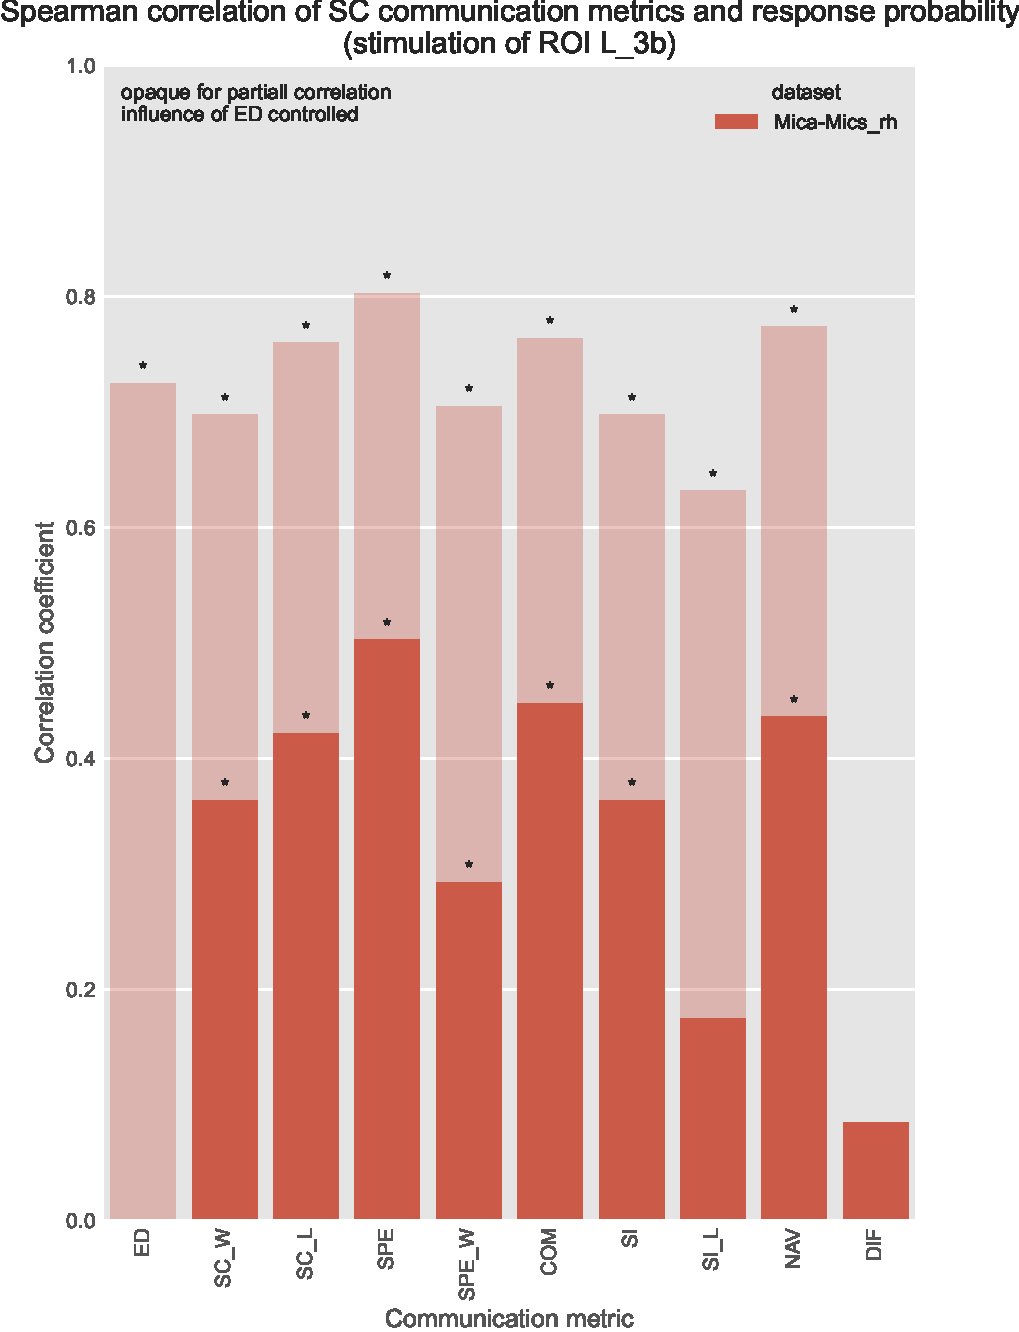
\includegraphics[width=\textwidth]{images/nootebook_generated/ftract_results_per_roi/long/MNI-HCP-MMP1/ED0/0.25/Spearman_correlation_of_SC_communication_metrics_and_response_probability_(stimulation_of_ROI_L_3b).pdf}
    \caption[F-TRACT probability correlations - Mica-Mics\_rh L\_3b]{Correlations (absolute value) of response probability (200~ms response) and structural connectivity and derived communication metrics. Asterisks denote a significant correlation ($p<0.05$).}
    \label{fig:ftract_mica_long_probabilities_L3b}
\end{figure}

The full correlations are overall even higher in this case than for the primary motor cortex stimulation (Figure \ref{fig:ftract_mica_long_probabilities_L4}) or the aggregated results (\ref{fig:ftract_mica_long_probabilities}). Regarding the communication metrics, the highest correlation is achieved with the shortest path efficiency (for both full and partial correlation), followed by communicability and navigation efficiency. Consistently with the previous results, the shortest path efficiency correlation with the probability response is higher than the correlation of the response with structural connectivity matrices.

The results for L\_4 and L\_3b confirm that it is reasonable to study correlations of stimulation responses with structural connectivity and communication metrics even if the stimulation was performed only at one site. That is an important finding, because TMS stimulation is often performed only at one site, and it is not possible to apply it to some ROIs (TMS can directly stimulate only 3 cm maximum depth from the surface of the head \cite{luber_using_2022}).
\chapter{Generalize F-TRACT approach to TMS-EEG}\label{ch:pytepfit}

The main goal of this thesis is to apply the approach by Seguin et al. \cite{seguin_communication_2023} rooted in complex network analysis and compare its applicability in empirical and simulated EEG recordings of TMS evoked potentials. As explained in Section \ref{sec:tms-eeg_measurement}, the TMS-EEG measurement is indirect; it does not require the implantation of electrodes in the brain. Because of that, it is easier to use it in research, but it is less precise. We want to see if it is possible to get an insight into the response structure using the communication models for TMS-EEG data similarly as it was presented in Sections \ref{sec:ftract_results} and \ref{sec:ftract_results_per_roi} for iEEG data. 

\section{TMS-EEG data}\label{sec:reponse_definition}

There are several key differences between the summarized iEEG functional data available in F-TRACT and the TMS-EEG data used in this section. 

The F-TRACT dataset provides probabilities. For each ROI, there is a vector of probabilities that there are significant responses in the other ROIs aggregated on a group level. On the other hand, the TMS-EEG data used here are time series of a single subject capturing the time-resolved response for each ROI after the target site stimulation. another difference is that the TMS-EEG data in the dataset used in this thesis were measured with stimulation on a single site, while F-TRACT includes stimulations in many different sites.

Besides empirical data, we work with simulated TMS-EEG data, and we compare the results. This comparison may be useful as guidance for the future development of models for a generation of artificial TMS-evoked responses.

\subsection{Empirical data}

We used TMS-EEG data published by the Rogasch group\footnote{\url{https://figshare.com/articles/dataset/TEPs-_SEPs/7440713}} \cite{biabani_characterizing_2019} where high-density EEG was recorded following M1 stimulation in 20 healthy young individuals. TMS-EEG evoked potential (TEP) source reconstruction was performed by Momi et al. \cite{momi_tms-evoked_2023}, resulting in group-averaged time series, one time series per ROI in Schaefer200 parcellation. See Figure \ref{fig:tms-empirical-data}. 

\begin{figure}
    \centering
    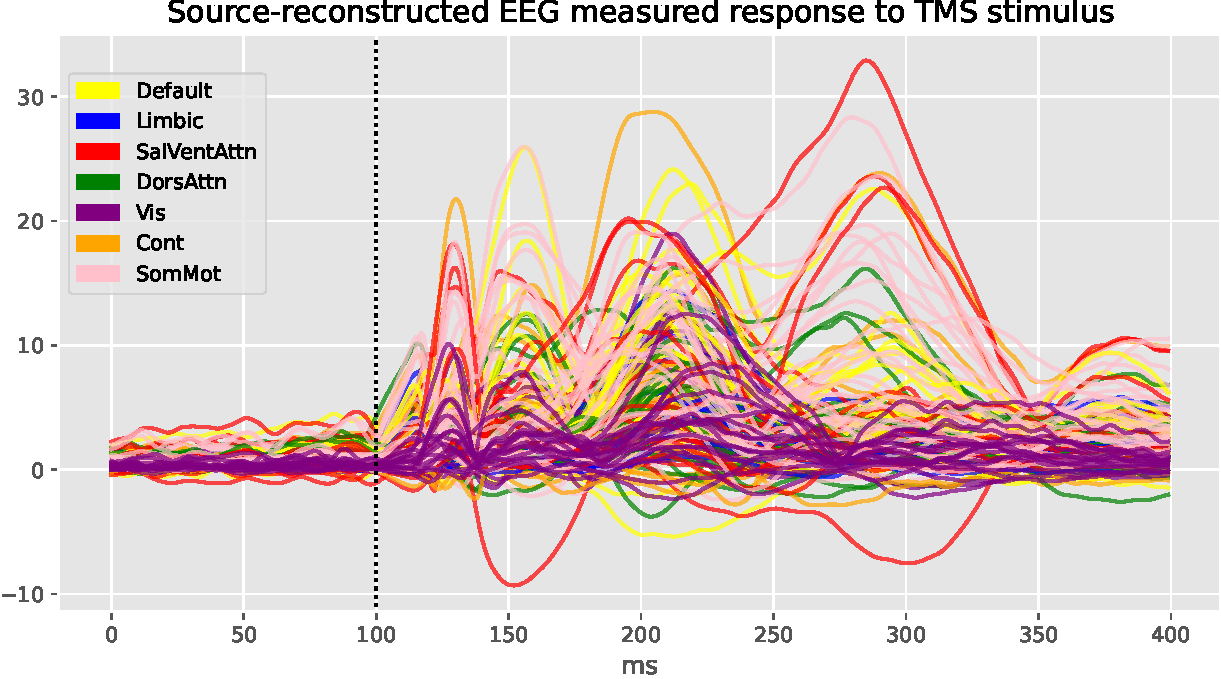
\includegraphics[width=\textwidth]{images/nootebook_generated/pytepfit_results/empirical/200/not_over_threshold_nan/data.pdf}
    \caption[TMS-EEG empirical data]{TMS-EEG empirical data, stimulation at 100 ms after the start of the measurement. The TEPs are colored based on Yeo7 functional networks. EEG source reconstructed, baseline corrected, and $z$-scored.}
    \label{fig:tms-empirical-data}
\end{figure}

\subsection{Simulated data}

Besides the source-reconstructed empirical TEPs, Momi et al. published simulated TEPs. The whole modeling process is described in their paper \textit{TMS-evoked responses are driven by recurrent large-scale network dynamics} \cite{momi_tms-evoked_2023}. 

Briefly, the model consists of 200 brain regions (based on Schaefer200 parcellation) connected by weights of some anatomical connectivity matrix. The nodes represent the averaged activity of the specific brain region and activity in each node is modeled using a set of equations. \cite{deco_perturbation_2018} Then, the model was fitted to the empirical data of each subject, and the resulting TEPs were averaged. \cite{momi_tms-evoked_2023}

The resulting simulated data are plotted in Figure \ref{fig:tms-simulated-data}. We see that the TEPs are much smoother than the empirical in Figure \ref{fig:tms-empirical-data}.

\begin{figure}
    \centering
    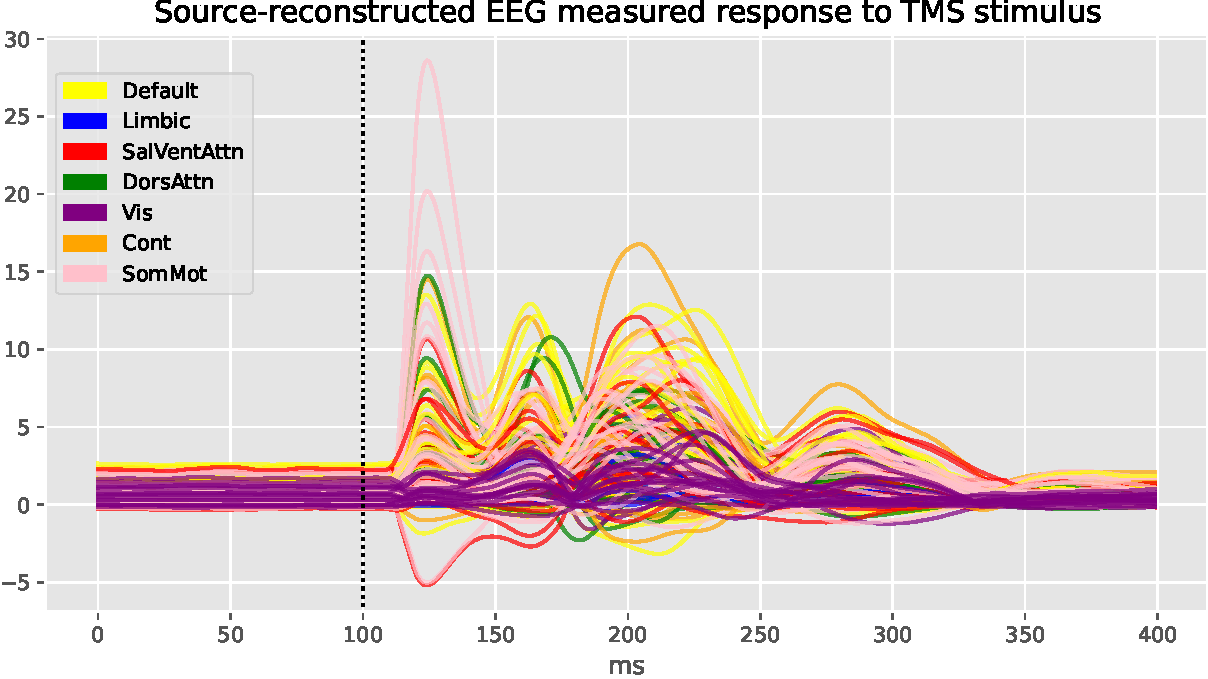
\includegraphics[width=\textwidth]{images/nootebook_generated/pytepfit_results/simulated/200/not_over_threshold_nan/data.pdf}
    \caption[TMS-EEG simulated data]{TMS-EEG simulated data, stimulation at 100 ms after the start of the measurement. The TEPs are colored based on Yeo7 functional networks. EEG source reconstructed, baseline corrected, and $z$-scored.}
    \label{fig:tms-simulated-data}
\end{figure}

\subsection{Quantification of TMS-EEG response}

To follow the methodology used by Seugin et al. for the F-TRACT data, it is necessary to decide how to quantify the time series of each ROI and, followingly, create a vector characterizing the response in the whole brain. We can not use the probability of the response because the TEPs were measured only in 20 subjects and we have the group-averaged data.

This section discusses all the options used later in the work.\footnote{We considered also variance, mean, difference of lowes and highest value, AUC of the area above the threshold, etc., but we did not include them because they are very similar to the ones in the list.} They are also visualized in Figure \ref{fig:tms-respondse-definition}.

\begin{itemize}
    \item \textbf{binary (01) response} If the TEP exceeds a predefined threshold, the value is set to 1, otherwise it is set to 0.
    \item \textbf{first/highest peak} The weight of the response is defined as the height of the first/highest peak above a predefined threshold. If the TEP does not exceed the threshold, it is set to \texttt{nan} and is not considered in the analysis.\footnote{Alternatively, we can replace all \texttt{nan}s in the definitions with zeros and include them in the analysis. The approaches capture different properties of the response.} The highest peak corresponds to amplitude in F-TRACT. 
    \item \textbf{first/highest peak time} The weight of the response is defined as the time when the first/highest peak above a predefined threshold occurs. If the TEP does not exceed the threshold, it is set to \texttt{nan} and is not considered in the analysis. The idea behind this definition is that we assume the response to propagate faster to regions that are \uv{more} connected (for example, there are edges with higher weights or shorter lengths in structural connectome).
    \item \textbf{AUC} The weight of the response is defined as the area under the curve if the curve exceeds a predefined threshold, \texttt{nan} otherwise. The key idea of this definition is that AUC captures the overall \uv{power} of the response. It is systematically different from the other definitions, so it might reveal different relationships.
\end{itemize}

\begin{figure}
    \centering
    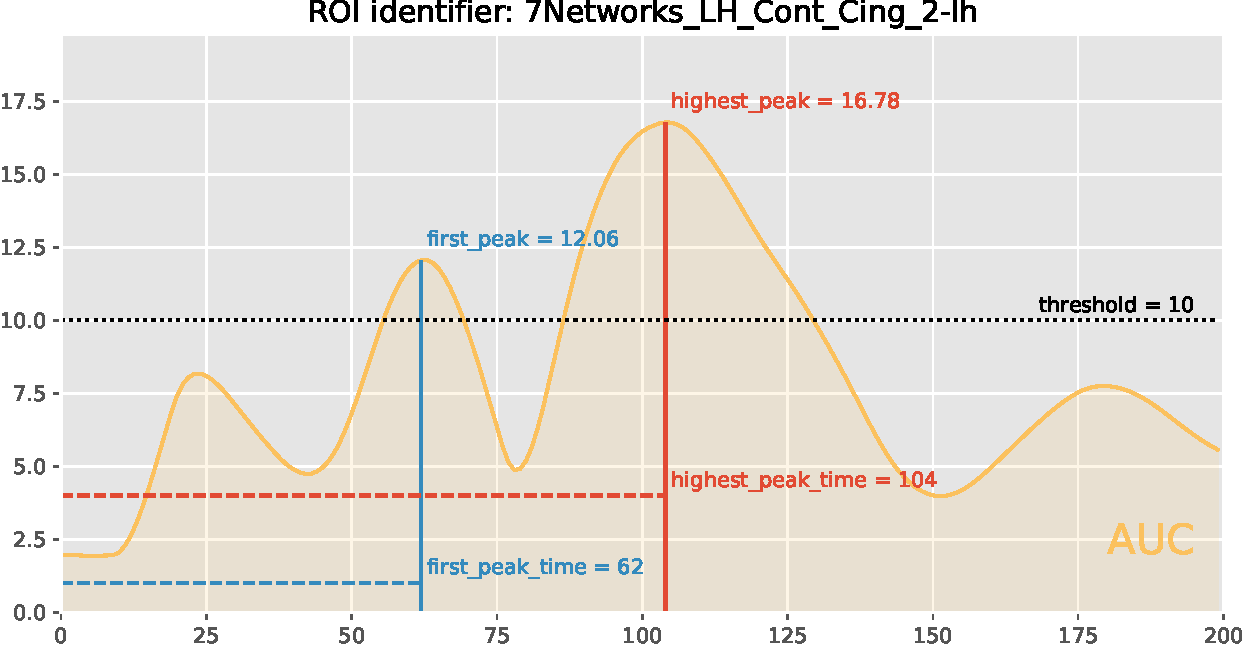
\includegraphics[width=\textwidth]{images/nootebook_generated/pytepfit_results/simulated/200/not_over_threshold_nan/7Networks_LH_Cont_Cing_2-lh_response_def.pdf}
    \caption[TMS-EEG response definitions -- illustration]{Definitions of the quantification of TMS-EEG response - illustration with one ROI, 200 ms response (stimulus at 0). EEG source reconstructed, baseline corrected, and $z$-scored.}
    \label{fig:tms-respondse-definition}
\end{figure}

\subsubsection{Threshold selection}

All the response definitions work with some threshold. There is always a baseline activity in the brain, as shown in Figure \ref{fig:tms-empirical-data} before the stimulation. We need to filter out the activity after the stimulation caused by this natural process and keep only responses truly evoked by the TMS stimulation. However, there is nothing like \uv{the right threshold} and it depends on the specific data used in each case. Because of that, we tried several thresholds, the lowest corresponding to the highest peak in the activity before the stimulation and the highest selected such that there are at least 30 TEPs over that threshold.

\subsubsection{Response length}

Besides the threshold, it is important to select the length of the response we want to consider. The later responses can be confounded by the auditory stimulus (loud TMS click), and somatosensory responses (activation of cranial nerves). \cite{hernandez-pavon_tms_2023} On the other hand, as shown in Section \ref{sec:response-length_F-Tract} the earlier responses might be driven simply by the Euclidean distance. We tried several response lengths, including 50 ms and 200 ms, which gave us results comparable to those obtained using F-TRACT.

\section{Results for empirical data}\label{sec:results_pytepfit-empirical}

In this section, we present the results showing that, for some of the response definitions (specifically binarized TEP, AUC, and first peak height), there are significant correlations across various thresholds between the response and structural connectivity and the communication metrics derived from it. 

For the structural connectivity, we used the Mica-Mics dataset with Rosen and Halgrens's preprocessing method because it gave us the best results for the F-TRACT dataset (Section \ref{sec:sc-robustness_ftract}) and it also provides the Schaefer200 parcellation used here, which allows better comparison of the results. We used the Spearman correlation coefficient, results are considered significant for $p<0.05$.

\subsection{Binarized response}

First, if the response is binarized, it correlates with Euclidean distance across response lengths 50, 100, 150, 200, and 300 milliseconds and various thresholds ($r \approx 0.4$ depending on the parameters). It serves as an assurance that the calculations are correct because Sections \ref{sec:ftract_results} and \ref{sec:ftract_results_per_roi} show that there is a high correlation between the response probability and amplitude and Euclidean distance. 

We show the results for 200 ms response across various thresholds in Figure \ref{fig:tms_01_200}. The shortest path efficiency and navigation efficiency correlations are similar to those achieved with Euclidean distance, similar to the F-TRACT results in Figure \ref{fig:ftract_alldata_long_probabilities}.

\begin{figure}
    \centering
    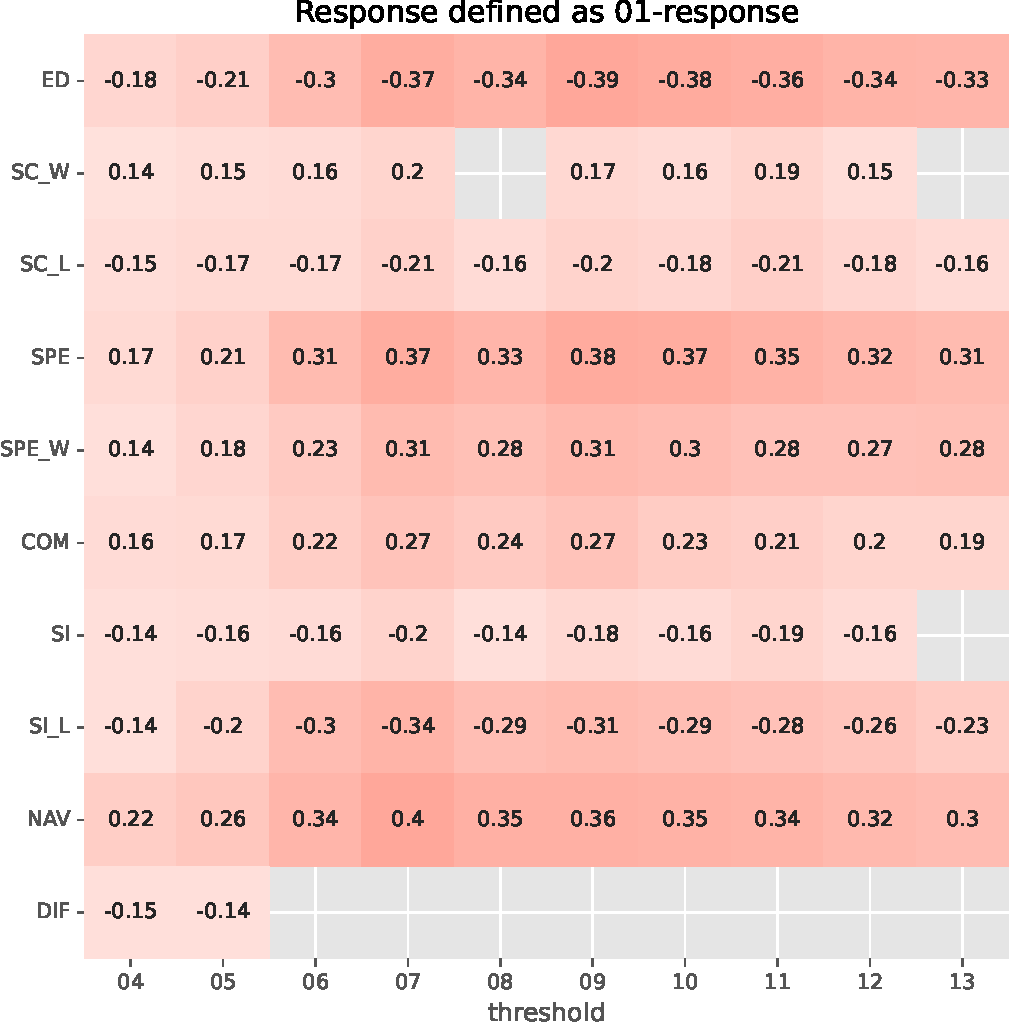
\includegraphics[width=\textwidth]{images/nootebook_generated/pytepfit_results/empirical/200/not_over_threshold_nan/Response defined as 01-response.pdf}
    \caption[Binarized TEP (200 ms) correlations]{Spearman correlation coefficient of binarized empirical TEP (200 ms response) with structural connectivity and communication metrics. Darker color denoted a higher absolute value of the correlation; missing values are non-significant ($p>0.05$).}
    \label{fig:tms_01_200}
\end{figure}

\subsection{Response characterized by AUC}

Based on our results, the AUC of TEP above a threshold correlates best with the structural connectivity and communication metrics.

The results for 50 ms response length (Figure \ref{fig:tms_auc_50}) differ from longer responses ($\geq100$ ms) because there are significant correlations consistently expressed only for Euclidean distance, shortest path efficiency, and navigation efficiency (and only for lower thresholds). For the longer responses (represented by Figure \ref{fig:tms_auc_200} for 200 ms), the correlations are overall higher and appear across various thresholds. 

Nevertheless, the response AUC correlation is consistently highest with Euclidean distance, the shortest path efficiency and navigation efficiency, followed by structural connectivity lengths, search information and communicability, which corresponds to the results in F-TRACT considering all pairs of ROIs (Figure \ref{fig:ftract_mica_short_probabilities} for 50 ms response and Figure \ref{fig:ftract_mica_long_probabilities} for 200 ms response).

\begin{figure}
    \centering
    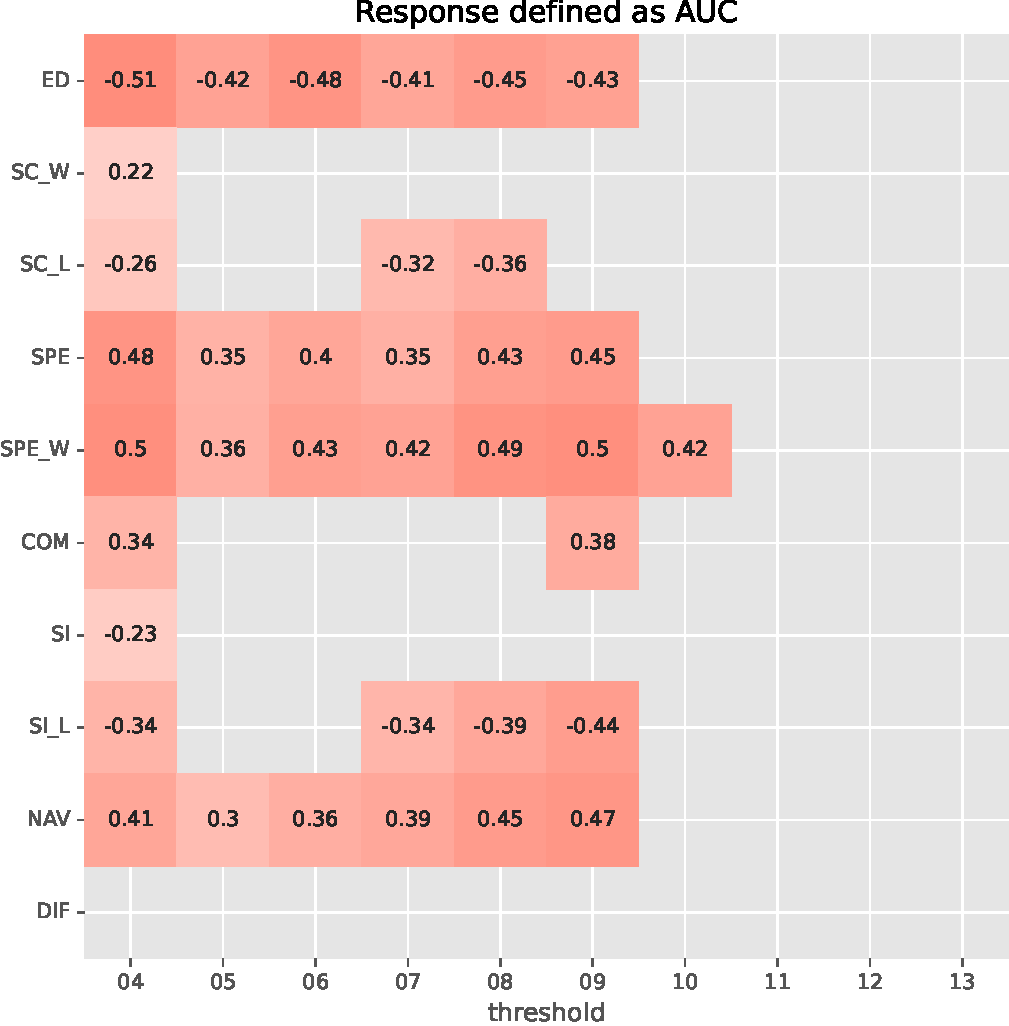
\includegraphics[width=\textwidth]{images/nootebook_generated/pytepfit_results/empirical/50/not_over_threshold_nan/Response defined as AUC.pdf}
    \caption[TEPs AUC (50 ms) correlation with SC and communication metrics]{Spearman correlation coefficient of AUC of empirical TEP (50 ms response) with structural connectivity and communication metrics. Darker color denoted a higher absolute value of the correlation; missing values are non-significant ($p>0.05$).}
    \label{fig:tms_auc_50}
\end{figure}

\begin{figure}
    \centering
    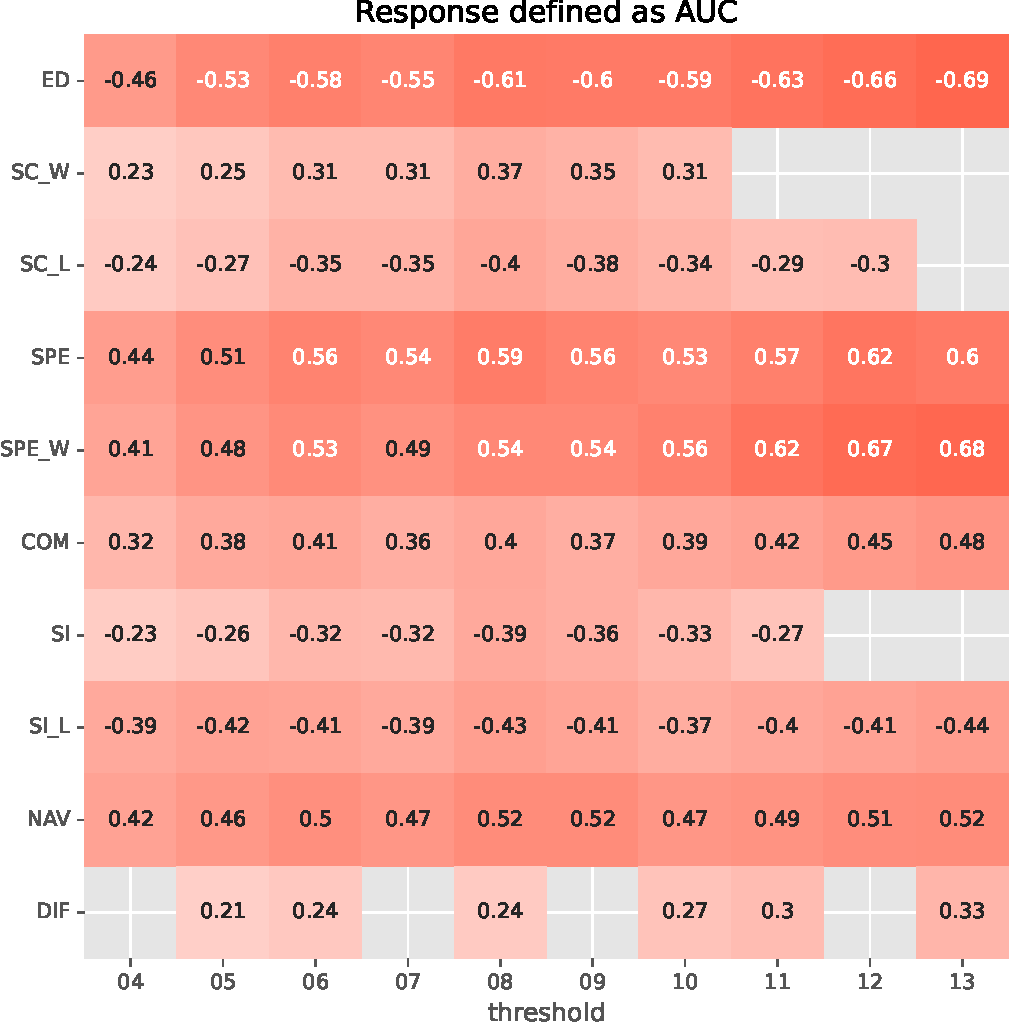
\includegraphics[width=\textwidth]{images/nootebook_generated/pytepfit_results/empirical/200/not_over_threshold_nan/Response defined as AUC.pdf}
    \caption[TEPs AUC (200 ms) correlations]{Spearman correlation coefficient of AUC of empirical TEP (200 ms response) with structural connectivity and communication metrics. Darker color denoted a higher absolute value of the correlation; missing values are non-significant ($p>0.05$).}
    \label{fig:tms_auc_200}
\end{figure}

\subsection{Response characterized by peak times}

If we characterize the response by the amount of time from the stimulation to the first peak, we need to consider an interval long enough so the peaks can occur. Looking at Figure \ref{fig:tms-empirical-data}, it could be seen that 50 ms is insufficient. Based on our experiments, we should take at least 150 ms response. 

Taking into account only responses longer than 150 ms, the first peak time correlates with Euclidean distance, shortest path efficiency, navigation efficiency, and communicability across all the thresholds. See Figure \ref{fig:tms_first_time_200} for 200 ms response.

\begin{figure}
    \centering
    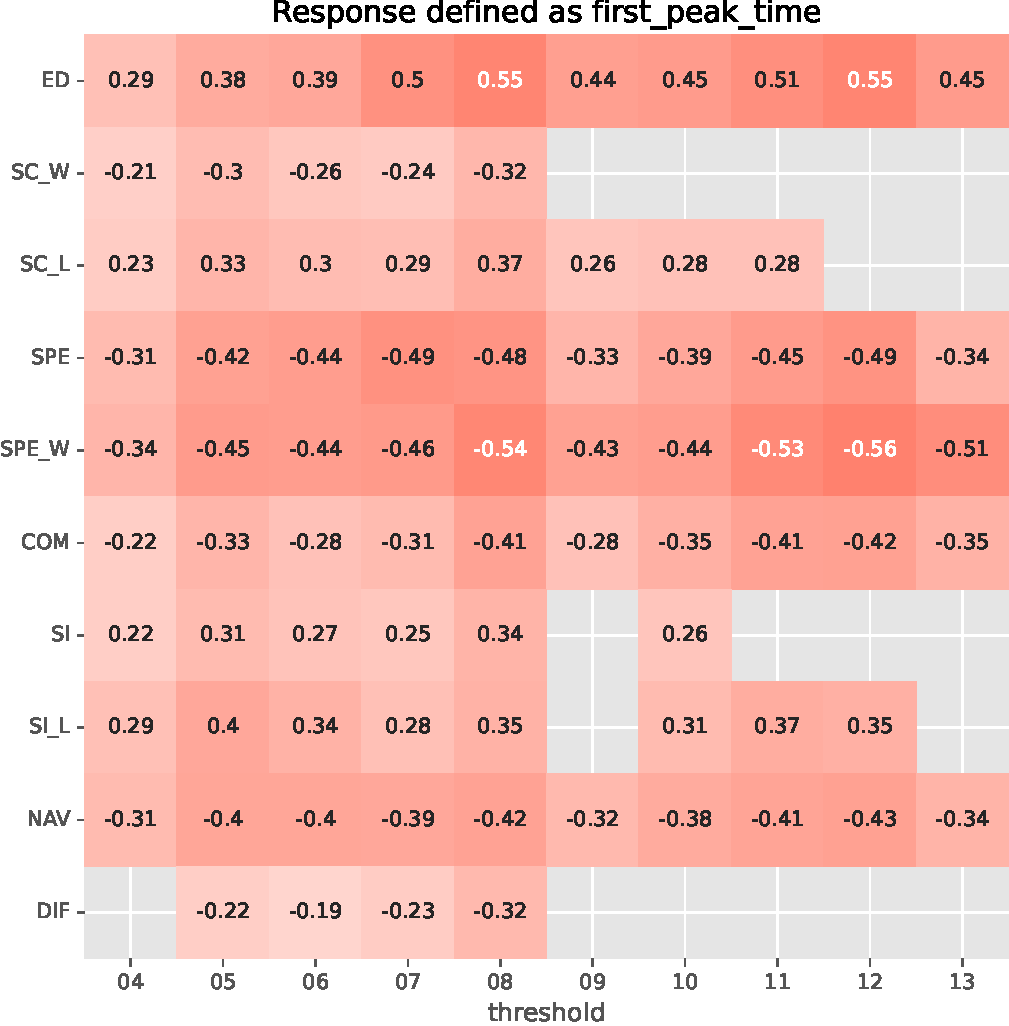
\includegraphics[width=\textwidth]{images/nootebook_generated/pytepfit_results/empirical/200/not_over_threshold_nan/Response defined as first_peak_time.pdf}
    \caption[TEPs first peak time (200 ms) correlations]{Spearman correlation coefficient of the first peak time in empirical TEP (200 ms response) with structural connectivity and communication metrics. Darker color denoted a higher absolute value of the correlation; missing values are non-significant ($p>0.05$).}
    \label{fig:tms_first_time_200}
\end{figure}

Characterizing the response by the highest peak time proved to be a dead end, as the results are largely non-significant. There is an exception for a response length of 150 ms, which shows many significant correlations. It is probably because the highest peaks correspond to the first peaks for this response length; the plot for this setting looks very similar to the first peak time responses shown in Figure \ref{fig:tms_first_200}. 

\subsection{Response characterized by peak heights}

Surprisingly, there are only a few significant correlations, only for lower thresholds, across all the response lengths when we use the highest peak as a response characterization. It seems that the relationship between the highest peak height and structural connectivity is weak, if any. It stands in contrast with the results obtained for response amplitudes from F-TRACT in Figure \ref{fig:ftract_alldata_long_amplitudes}, where we see significant correlations of the amplitudes with structural connectivity and communication metrics. See Figure \ref{fig:tms_heighest_200} for 200 ms response.

The height of the first peak does not exhibit any correlations with structural connectivity and communication metrics at all. 

\begin{figure}
    \centering
    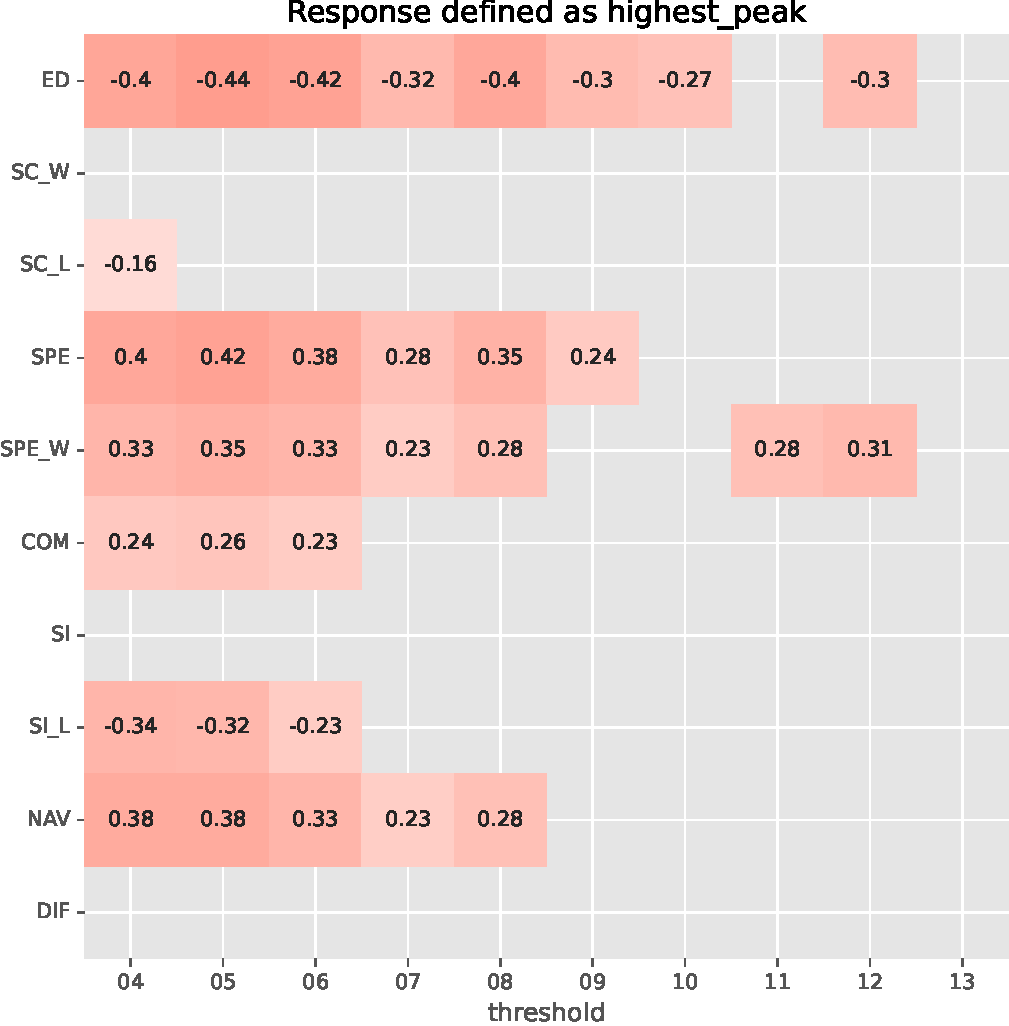
\includegraphics[width=\textwidth]{images/nootebook_generated/pytepfit_results/empirical/200/not_over_threshold_nan/Response defined as highest_peak.pdf}
    \caption[TEPs highest peak (200 ms) correlations]{Spearman correlation coefficient of the height of the highest peak in empirical TEP (200 ms response) with structural connectivity and communication metrics. Darker color denoted a higher absolute value of the correlation; missing values are non-significant ($p>0.05$).}
    \label{fig:tms_heighest_200}
\end{figure}

\subsection{Response length}

The results change with response length. As mentioned above, if the response is characterized by the first peak time, the length should be at least around 150 ms. If the response is shorter, not all peaks occur in the time. 

If we characterize the response using AUC, the results for a really short response length (50 ms) are different from the other response lengths ($\geq100$ ms), as shown in Figure \ref{fig:tms_auc_50} and Figure \ref{fig:tms_auc_200}.

\section{Empirical vs simulated data}

The main question we aim to answer by comparing results for empirical and simulated data is if the simulated data express similar behavior to the empirical ones. We can see just by looking at Figures \ref{fig:tms-empirical-data} and \ref{fig:tms-simulated-data} that the distribution, height, and timing of the peaks and AUC are different. 

Does it mean that the data act differently concerning the analysis of the response correlation with structural connectivity and communication metrics? The possible similarity of the results could mean that the simulated data grasps some aspects of the empirical data and we can study the simulated data to reveal some aspects of the nature of the brain.

\subsection{Similarities}

The first important similarity lies in the results for the binarized response. It shows the same pattern as we have seen before, the response correlates with Euclidean distance, the shortest path efficiency, and the navigation efficiency. Figure \ref{fig:tms_binary_100_simulated} shows that for 100 ms response. 

\begin{figure}
    \centering
    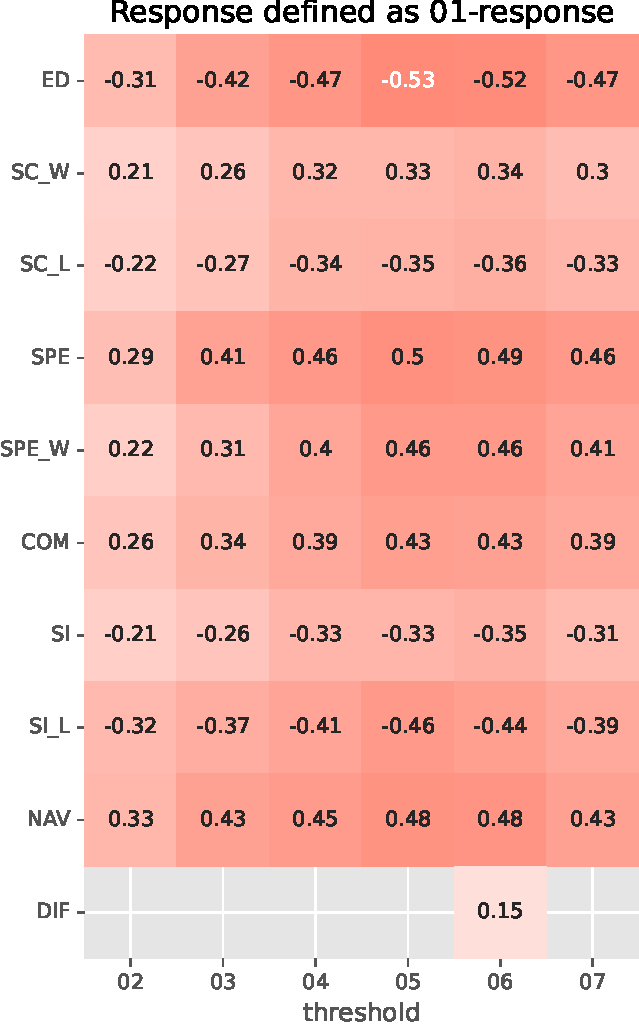
\includegraphics[height=\textwidth]{images/nootebook_generated/pytepfit_results/simulated/100/not_over_threshold_nan/Response defined as 01-response.pdf}
    \caption[Binarized TEP (100 ms) correlations (simulated data)]{Spearman correlation coefficient of binarized empirical TEP (100 ms response) with structural connectivity and communication metrics. Darker color denoted a higher absolute value of the correlation; missing values are non-significant ($p>0.05$).}
    \label{fig:tms_binary_100_simulated}
\end{figure}

Another similarity can be found in the response characterized by the first peak time. Even though the correlations are overall higher for simulated data, Figure \ref{fig:tms_first_time_200_simulated} shows a similar pattern to Figure \ref{fig:tms_first_time_200} with the highest correlations of the first peak times with Euclidean distance, shortest path efficiency and navigation efficiency across all thresholds. 

\begin{figure}
    \centering
    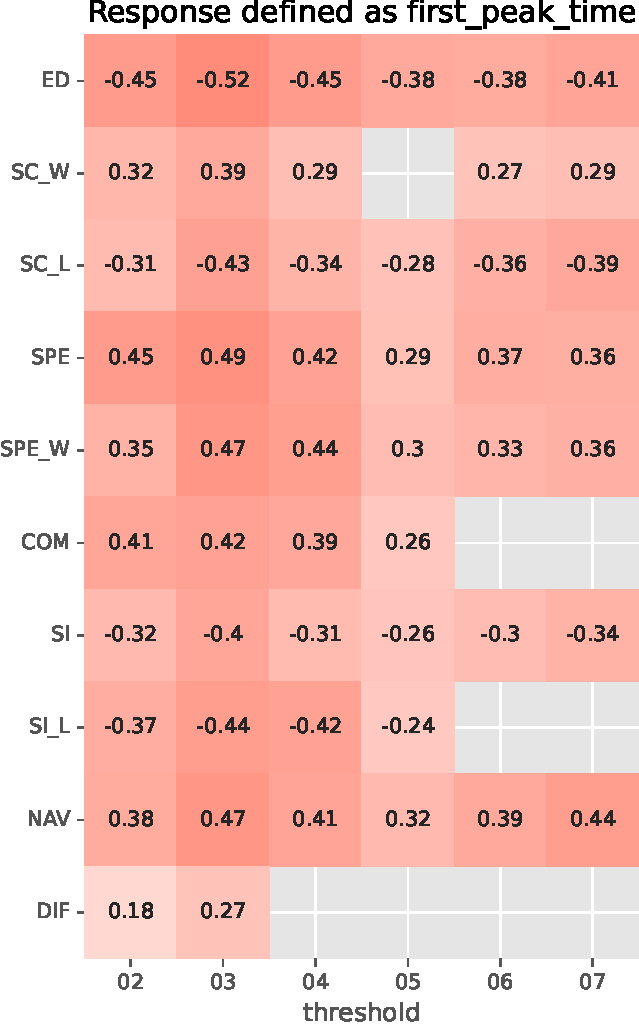
\includegraphics[height=\textwidth]{images/nootebook_generated/pytepfit_results/simulated/200/not_over_threshold_nan/Response defined as first_peak_time.pdf}
    \caption[TEPs first peak time (200 ms) correlations (simulated data)]{Spearman correlation coefficient of the first peak time in simulated TEP (200 ms response) with structural connectivity and communication metrics. Darker color denoted a higher absolute value of the correlation; missing values are non-significant ($p>0.05$).}
    \label{fig:tms_first_time_200_simulated}
\end{figure}

\subsection{Differences}

Unsurprisingly, there are many differences in the results calculated using simulated and empirical data. First of all, considering a response length of at least 100 ms, the highest correlations of the response with communication metrics are obtained for response strength defined as its highest peak time (Figure \ref{fig:tms_highest_time_200_simulated} for 200 ms response).

\begin{figure}
    \centering
    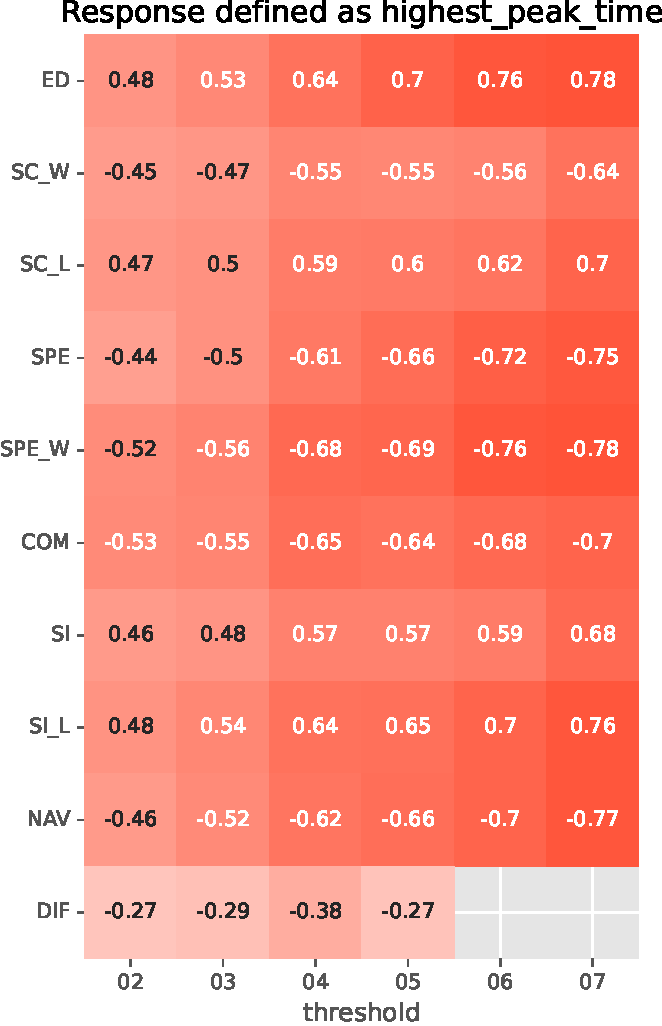
\includegraphics[height=\textwidth]{images/nootebook_generated/pytepfit_results/simulated/200/not_over_threshold_nan/Response defined as highest_peak_time.pdf}
    \caption[TEPs highest peak time (200 ms) correlations (simulated data)]{Spearman correlation coefficient of the highest peak time in simulated TEP (200 ms response) with structural connectivity and communication metrics. Darker color denoted a higher absolute value of the correlation; missing values are non-significant ($p>0.05$).}
    \label{fig:tms_highest_time_200_simulated}
\end{figure}

Response characterized by AUC correlates much worse with structural connectivity and communication metrics if it is calculated using the simulated data, as shown in Figure \ref{fig:tms_AUC_200_simulated}. On the other hand, the height of the peaks correlates better with communication metrics for the simulated data than for the empirical data (but worse than other response characteristics for simulated data). 

\begin{figure}
    \centering
    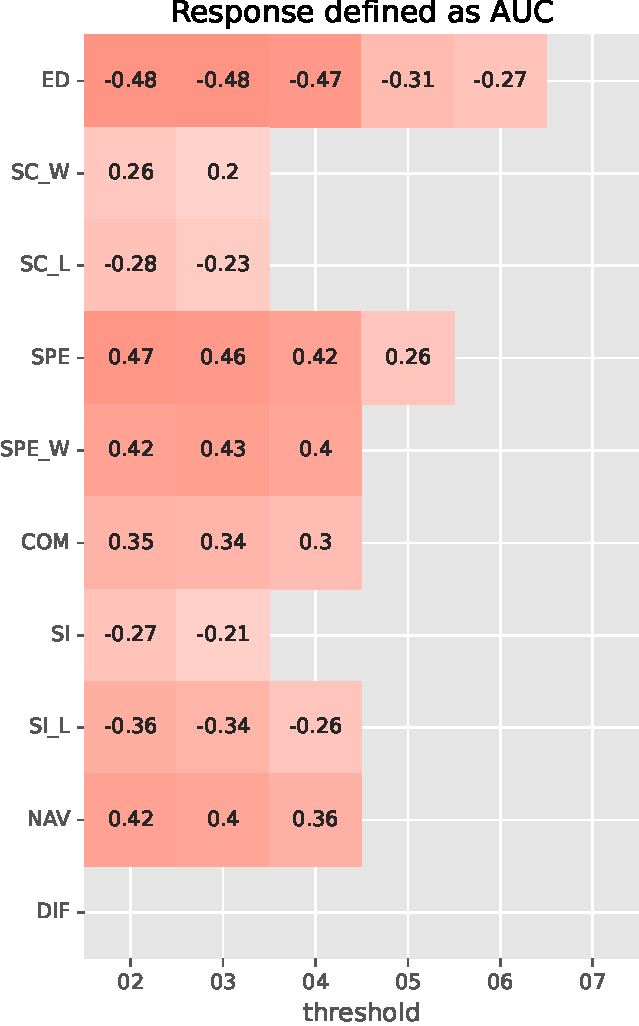
\includegraphics[height=\textwidth]{images/nootebook_generated/pytepfit_results/simulated/200/not_over_threshold_nan/Response defined as AUC.pdf}
    \caption[TEPs AUC (200 ms) correlations (simulated data)]{Spearman correlation coefficient of AUC of simulated empirical TEP (200 ms response) with structural connectivity and communication metrics. Darker color denoted a higher absolute value of the correlation; missing values are non-significant ($p>0.05$).}
    \label{fig:tms_AUC_200_simulated}
\end{figure}

In conclusion, the similarities and differences seem to follow the difference in data simulation and generation through the natural process in the brain. The simulated data capture the highest peak timings, which might be noisy in the empirical data. On the other hand, the simulated data probably do not model very well the overall complexity of the response, captured by AUC in the empirical data. 

The correlations with communication models are overall higher for simulated data. This might be because of the lower noise, but also because of the lack of more complex interactions in the modeled data. The model is a simplified description of the complex process, which might result in higher correlations with the simplified description of the communication using communication models. 

All the differences could be used for the next iteration of TMS-EEG simulating model development.
\chapter{TMS-EEG and F-TRACT comparison}\label{ch:compare}

This chapter is devoted to the following questions: If we use TMS-EEG instead of iEEG (used in F-Tract), does the response still correlate with structural connectivity and communication metrics?  What are the similarities and what are the discrepancies? 

\section{Comparison of the correlations}\label{sec:compare-correlations_F-Tract-TMS}

Figure \ref{fig:compare-correlations_F-Tract-TMS} shows together the correlation coefficients of response probability or other characteristics with structural connectivity and communication metrics for 200 ms responses. 

TMS-EEG correlations are lower than correlations for F-Tract, no matter how we characterize the response. That was expected because the TMS stimulation has to get through the skull and other tissues before it enters the target region, and also the EEG measurement is performed through the head and source-reconstructed afterward, which all adds noise to the data.

Looking at the communication metrics, both TMS-EEG and F-TRACT correlate best with the shortest path efficiency. An interesting observation is that if the response is characterized by first peak height, it correlates better with shortest path efficiency calculated using structural connectivity weights than lengths.

Another interesting question is how much can be explained by the Euclidean distance of the regions. As discussed in Chapter \ref{ch:ftract}, there are significant partial correlations for F-TRACT probabilities and amplitudes even when Euclidean distance is controlled. We can also see in Figure \ref{fig:compare-correlations_F-Tract-TMS} that some of the communication metrics achieve higher correlations with response probability than the Euclidean distance for F-Tract. None of this is true for the TMS-EEG data. There are no significant partial correlations and the correlations of responses with communication metrics are lower than with Euclidean distance.\footnote{It is like that also for the other TMS-EEG thresholds and response lengths discussed in Chapter \ref{ch:pytepfit}.} 

This means that even though we might get some insight by studying the TMS-EEG from the perspective of communication metrics, we should keep in mind that various aspects of the response (AUC, the first peak height) are largely driven by the Euclidean distance. 

\begin{figure}
  \begin{center}
    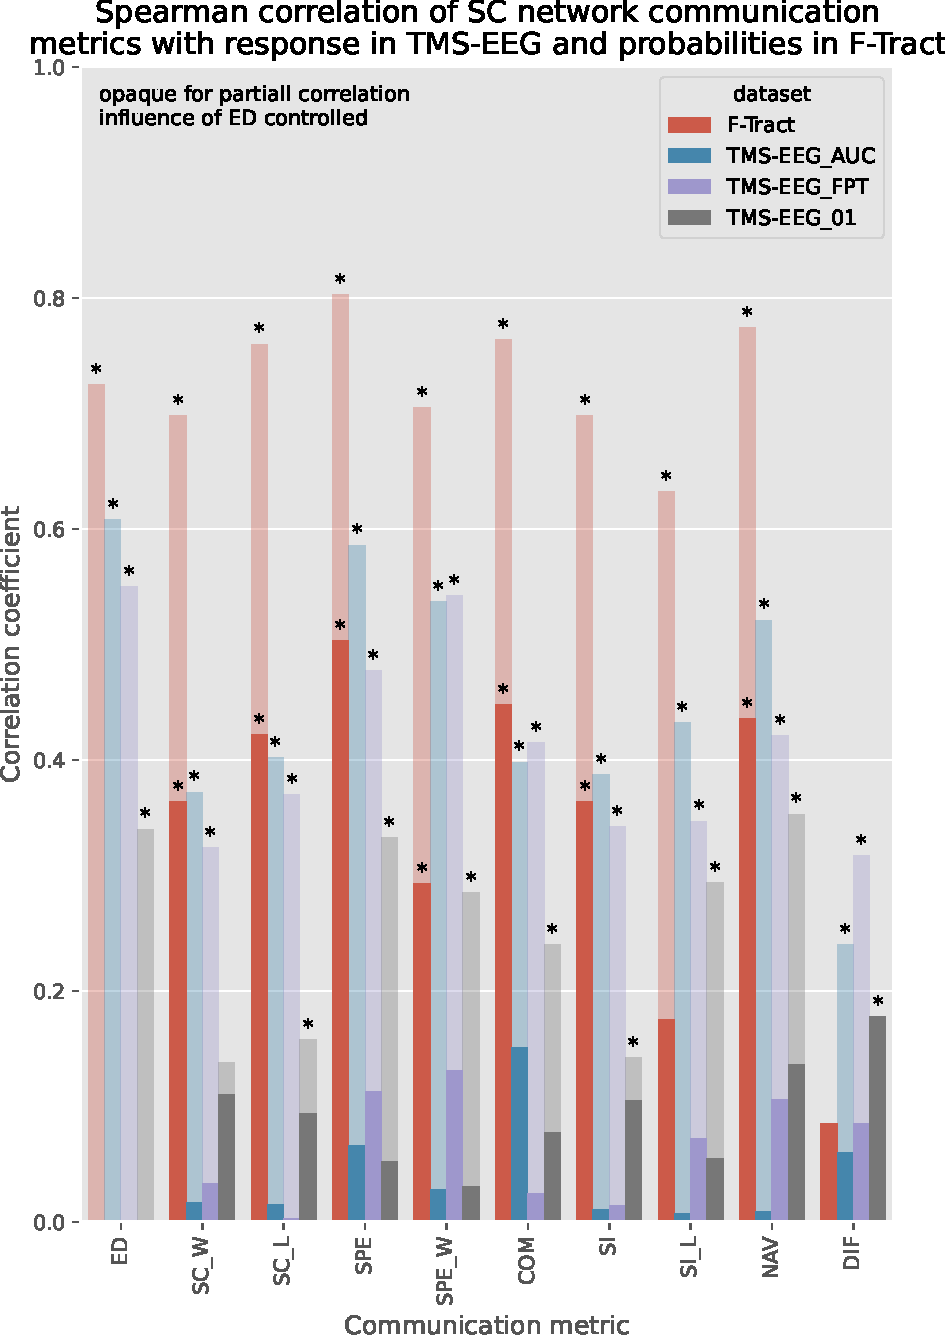
\includegraphics[width=0.89\textwidth]{images/nootebook_generated/pytepfit_ftract_comparison_results_200ms/Spearman_correlation_of_SC_network_communication_metrics_with_response_in_TMS-EEG_and_probabilities_in_F-Tract.pdf}
  \end{center}
  \caption[Comparison of correlations for F-Tract and TMS-EEG]{Comparison of correlations (absolute value) of response probability in F-Tract and TMS-EEG response characterized binary (01), by AUC and by the first peak latency (FPT) and structural connectivity and derived communication metrics. Asterisks denote a significant correlation ($p<0.05$). All the responses 200 ms long, structural connectivity based on Mica-Mics dataset with Rosen and Halgren's preprocessing. Threshold 8 in $z$-scored TMS-EEG.}
  \label{fig:compare-correlations_F-Tract-TMS}
\end{figure}

\section{Parcellations mapping}\label{sec:dice}

Direct comparison of the TMS-EEG and F-TRACT results is not possible, because they do not share the same brain parcellation. The TMS-EEG dataset is published in Schaefer200 parcellation, which is not available for F-TRACT. Because of that, it is necessary to find a mapping between Glasser and Schaefer200 parcellation.

Lawrence et al. published a paper \textit{Standardizing human brain parcellations} \cite{lawrence_standardizing_2021} discussing the issue of mapping between distinct brain parcellations. They propose the Dice coefficient \cite{dice_measures_1945} as a possibility of similarity evaluation between ROIs across parcellations. 

For two ROIs $A$ and $B$, each consisting of a set of voxels, the Dice coefficient of association is calculated as  
$$
\frac{2 \cdot |A\cap B|}{|A|+|B|}.
$$
the score is a ratio of the overlap of the regions to the sum of their sizes. It is higher for regions with a big overlap with respect to their sizes.

Lawrence et al. provide a function for calculations of Dice scores between parcellations in Neuroparc repository at GitHub.\footnote{\url{https://github.com/neurodata/neuroparc/blob/5a5e7469671e65cb58087c47b69d0edb71dc2966/scripts/dice_correlation.py}} Using that, Dice score map between Schaefer200 and Glasser parcellations was created.

Having the matrix with Dice scores for each pair of ROIs from Schaefer200 and Glasser, the easiest way to get comparable results is to assign one Schaefer200 ROI to each Glasser ROI based one the highest Dice coefficient (or vice versa, assign Glasser to Schaefer200 ROI). We can use this as a mapping for the vector of response probabilities in F-Tract and response AUC or other characteristics in TMS-EEG. 

\subsection{Stimulated site}\label{sec:parcellations-mapping-stimulated_roi}

Diving into the mapping of the parcellations, we found a discrepancy in the TMS-EEG data. The data-describing paper by Biabani et al. \cite{biabani_characterizing_2019} declares they stimulated the primary motor cortex, which is denoted \texttt{4\_L} in Glasser parcellation. Using the Dice mapping, this region has the highest overlap with ROI \texttt{7Networks\_LH\_SomMot\_15} in Schaefer200 parcellation. 

However, the source-reconstruction of the TMS-EEG data by Momi et al. \cite{momi_tms-evoked_2023} contains a vector indicating the stimulation weights for ROIs in Schaefer200. According to that, the stimulation target was \texttt{7Networks\_LH\_SomMot\_9} and \texttt{7Networks\_LH\_SomMot\_10} was affected a bit. Using the Dice scores again, ROI \texttt{7Networks\_LH\_SomMot\_9} has the biggest overlap with ROI \texttt{1\_L} in Glasser parcellation, followed by \texttt{3b\_L}. It has no overlap with ROI \texttt{4\_L}.

Because we use the TMS-EEG data in Schaefer200 parcellation, we decided to use \texttt{3b\_L} as a corresponding stimulation site in Glasser for the analysis, even though it is not the primary motor cortex. We chose \texttt{3b\_L} instead of \texttt{1\_L} because they are close to each other, both have an overlap with \texttt{7Networks\_LH\_SomMot\_9} and there are much more data in F-Tract for \texttt{3b\_L} stimulation than for \texttt{1\_L} stimulation, which is better for the analysis. 

\subsection{Comparison of F-TRACT and TMS-EEG responses}

Section \ref{sec:compare-correlations_F-Tract-TMS} discusses that there are similarities in correlations between the stimulus responses in F-TRACT and TMS-EEG and communication metrics. Now, let us see the relationship between responses in F-TRACT and TMS-EEG. Are the responses structurally similar? If the same site is stimulated, does the strength of activation in TMS-EEG correspond to the response probability in F-TRACT?

There is a significant correlation between AUC in TMS-EEG and response probability (Spearman correlation coefficient is $r=0.60$). If we look at the first peak height instead of AUC, there is again a significant correlation with the probability (Spearman correlation coefficient $r=-0.56$). The correlation is negative -- the responses with higher probabilities occur faster. 

Figure \ref{fig:response_tmsAUC-ftract_scatter} shows the response probability in F-TRACT vs AUC in TMS-EEG. We see that there are regions in the somatomotor area that have a high probability of activation but the value of AUC is not exceptionally high and, on the contrary, regions in the salience/ventral attention area that do not have that high probability of activation according to F-Tract, but very high AUC. Figure \ref{fig:response_tmsFP-ftract_scatter} shows the comparison for the first peak latency instead of AUC. 

\begin{figure}
  \begin{center}
    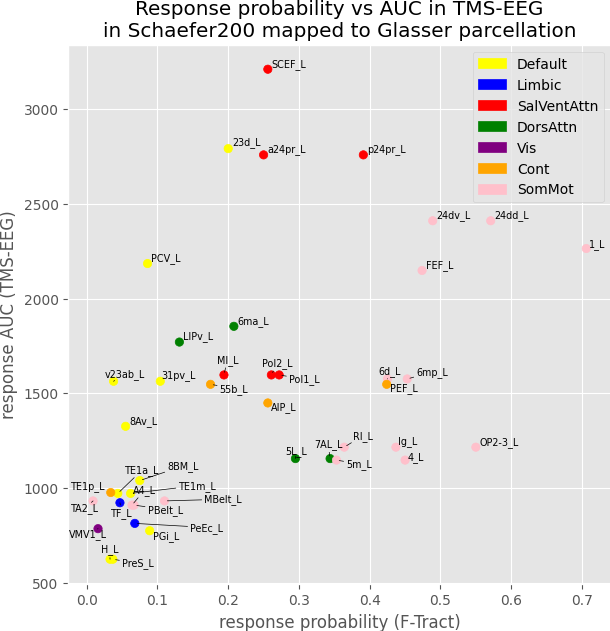
\includegraphics[width=\textwidth]{images/nootebook_generated/pytepfit_ftract_comparison_results_200ms/AUC/Response_probability_vs_AUC_in_TMS-EEG_in_Schaefer200_mapped_to_Glasser_parcellation.png}
  \end{center}
  \caption[F-TRACT probabilities vs TMS-EEG AUC]{F-TRACT probabilities vs TMS-EEG AUC for 200 ms response length and threshold 8 in TMS-EEG. ROIs labeled based on Glasser parcellation and colored based on Yeo7 network extracted from Schaefer200 parcellation, plotted if the response value not \texttt{nan} in both F-TRACT and AUC. Each Glasser ROI was assigned to Schaefer200 ROI based on the highest Dice score.}
  \label{fig:response_tmsAUC-ftract_scatter}
\end{figure}

\begin{figure}
  \begin{center}
    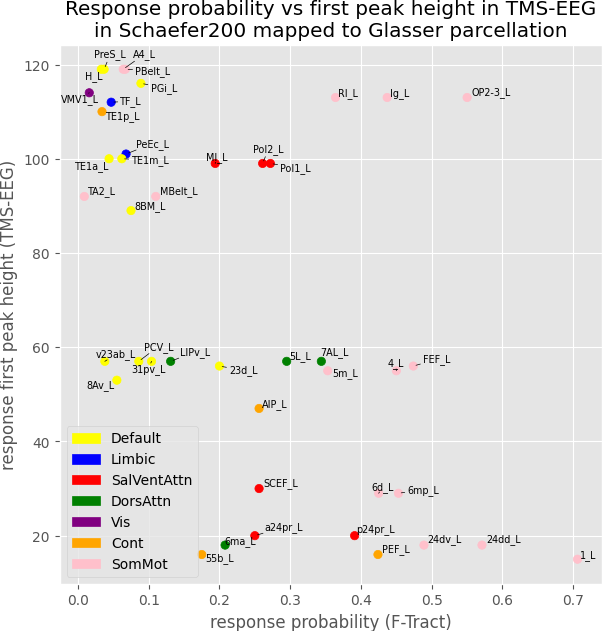
\includegraphics[width=\textwidth]{images/nootebook_generated/pytepfit_ftract_comparison_results_200ms/FP/Response_probability_vs_first_peak_height_in_TMS-EEG_in_Schaefer200_mapped_to_Glasser_parcellation.png}
  \end{center}
  \caption[F-TRACT probabilities vs TMS-EEG first peak latency]{F-TRACT probabilities vs TMS-EEG first peak latency for 200 ms response length and threshold 8 in TMS-EEG. ROIs labeled based on Glasser parcellation and colored based on Yeo7 network extracted from Schaefer200 parcellation, plotted if the response value not \texttt{nan} in both F-TRACT and AUC. Each Glasser ROI was assigned to Schaefer200 ROI based on the highest Dice score.}
  \label{response_tmsFP-ftract_scatter}
\end{figure}
\chapter{Connectomes variations and  robustness}\label{ch:SC_indepth}

All the presented results up to this point (with an exception in Chapter \ref{ch:ftract}) were obtained with structural connectivity matrices created using Rosen and Halgren's averaging method from Mica-Mics dataset. Let us look closer at the possible group-averaging methods and possible variations in structural matrices based on the data source and group-averaging methods. 

\section{Minimal number of streamlines}

Having a structural connectivity matrix containing streamline counts as described in Section \ref{sec:edge_estimation}, we have to decide if it is enough to have one streamline connecting two regions to consider it as an edge. For example, Seguin et al. \cite{seguin_communication_2023} decided to prune connections comprising fewer than 5 streamlines. They justify this step with the high false positive rate of probabilistic tractography. Following their example, we did the same. In all the following group-averaging methods, we first discarded subject-level edges with less than 5 streamlines.

\section{Group-average structural connectome construction}\label{sec:group-avg}

Assume we already have a connectivity matrix for each subject in some group, edge weights representing streamline count. Because we want to work with the general structural properties of the brain, the question of constructing a group-representative connectome arises. Group averaging aims to increase the signal-to-noise ratio and obtain a clearer picture of brain network organization in general while preserving network properties that are consistently expressed at the subject level (such as edge length distribution). \cite{betzel_distance-dependent_2019} In this section, we present some possible approaches.

\subsection{Simple average}\label{sec:average}

The most straightforward idea is to average the streamline count between each pair of nodes across all the subjects. The main problem with this approach is that whenever there is at least one subject with an edge from A to B, the AB average is always non-zero, suggesting that \enquote{there is a connection between these nodes}. As a result, the network density might be higher in the averaged connectome. That is an issue, especially because the process of obtaining streamline counts is erroneous, and the presence of one subject with this edge might be an accident.

\subsection{Consensus thresholding}\label{sec:cons-thr}

Consensus thresholding is the most common approach. It tries to preserve features consistently expressed at individual subjects' level while reducing noise. Threshold $\tau$ between 0 and 1 is specified\footnote{There is no consensus about the \enquote{correct} value of $\tau$ and it is often selected according to some heuristics. That might be a source of complications while attempting to compare connectomes across different studies.}, and the connections that are observed in at least $\tau$ fraction of subjects are kept. These connections are associated with weight, for example, the average number of streamlines among the subjects where the connection is present. The rest is set to 0. \cite{betzel_distance-dependent_2019}

Betzel et al. point out that this approach favors shorter edges which are easier to reconstruct using tractograpy. Consequently, the distribution of edge lengths is different in average connectome than in the single subjects. According to their argumentation, the longer edges are less common, but despite that, they have an important function in the brain. On the grounds of that, it is important to keep the edge length distribution because structural networks need long-distance connections. They propose their own method to prevent the issue, and we present it below. \cite{betzel_distance-dependent_2019} 

\subsection{Distance-dependent consensus thresholding}\label{sec:dist-dep}

This method aims to preserve edge length distribution. Assume the list of edges and their lengths. \footnote{Lengths might be Euclidean distances of the nodes or some sort of streamline average lengths.} Let us define $M$ as the total number of edges we want to keep in the consensus network. We define $M$ bins based on edge length percentiles. For each of them, we find all possible edges falling into that bin by length. For each bin, we choose the edge that is expressed most often across the subjects with ties broken by the greatest average weight (for example, streamline count). \cite{betzel_distance-dependent_2019} 

We used \texttt{struct\_consensus} method from netneurotools package\footnote{\url{https://netneurotools.readthedocs.io/en/latest/index.html}} for Python for calculation of distance-dependent thresholding during the work on this thesis.

\subsection{Averaging by Rosen and Halgren}\label{sec:rh}

This method was used by Rosen and Halgren in the paper \textit{A Whole-Cortex Probabilistic Diffusion Tractography Connectome} \cite{rosen_whole-cortex_2021} in a group-averaging of the matrix described in Section \ref{sec:rhdata}.

The principle is the same as a simple average, but it works with a ratio of streamlines between two parcels to a global number of streamlines instead of plain streamline counts. According to the paper, the values are first averaged across the subjects and then scaled such as the number of streamlines originating at parcel A and terminating at parcel B is divided by the total number of streamlines that either originate at parcel A or terminate at parcel B, excluding within-parcel connections. \cite{rosen_whole-cortex_2021} We used the equation below, where $SC$ is the final structural connectivity matrix and $m$ is an average of structural matrices across individual subjects.

$$
SC_{ij} = \frac{m_{ij}}{\sum_k m_{ik} + \sum_l m_{lj} - (m_{ii} - m_{jj})}
$$

In practice, he resulting matrix was sometimes non-symmetric even if the individual subject matrices were symmetric. It was caused by numerical instability in Python while working with small numbers. To overcome this problem, we added $SC = (SC + SC^T) /2$ to the end of the procedure.

\section{Structural connectome density}

Seguin et al. \cite{seguin_communication_2023} in the paper \textit{Communication dynamics in the human connectome shape the cortex-wide propagation of direct electrical stimulation} propose one more step in connectome construction. They prune the group-averaged connectivity matrices keeping the edges with the highest weight such that the density of the connectome is 25\%. 

The density of structural connectivity matrices differs across da\-ta\-sets, it depends on the individual connectome construction parameters. For example, the average connection density in Mica-Mics dataset is  84.1\% across subjects. \cite{seguin_communication_2023} If we want to get comparable results, it is necessary to start with connectomes with similar density. Because of that, we decided to threshold all the group-average matrices and keep approximately 25\% strongest edges.\footnote{Seguin et al. thresholded the subject-level matrices, but we do not have those available for some of the datasets. Because of that, we decided to do this step later to get the same density for all structural connectivity matrices.}

\section{Structural connectomes description}

All structural connectomes used during our work are described in this section. Some of them were published as group-averaged, while others came as a set of single-subject matrices. This section presents how they were constructed and compares them. 

\subsection{Enigma}\label{sec:enigma}

The first source of structural connectivity matrices for this thesis is a Python package ENIGMA TOOLBOX\footnote{\url{https://enigma-toolbox.readthedocs.io/en/latest/}, accessed 1. 5. 2024} developed by S. Larivière and B. Bernhardt from MICA Lab - Montreal Neurological Institute \cite{lariviere_enigma_2020}. It provides an option to load structural connectivity matrices in several parcellations. The original data were taken from 207 healthy adults from the HCP dataset.\footnote{The Human Connectome Project (HCP) is a large scientific effort focused on mapping the connectivity of the human brain. The HCP datasets are openly available to researchers at \url{https://www.humanconnectome.org/}. \cite{van_essen_human_2012}} The preprocessing pipeline is described in detail in a paper \textit{The ENIGMA Toolbox: Cross-disorder integration and multiscale neural contextualization of multisite neuroimaging datasets} by Larivière et al. For our application, it is important to note that the group average structural connectome was obtained using a distance-dependent thresholding procedure described above~\ref{sec:dist-dep}. Afterward, it was log-transformed. The structural connectomes are available in DK, Glasser, and Schaefer parcellations. 

There is a disadvantage of Enigma structural matrices, they provide only edge weights, not lengths. It is also important to mention that for Glasser and Schaefer parcellations, there are no zero weights in the matrix, but most of it is filled with ones (which is not the case for the DK parcellation) -- connectome is a complete graph with weights mostly one.

\subsection{Domhof}\label{sec:domhof}

This dataset, created by Domhof et al. \cite{domhof_parcellation-based_2022}, is available online on the EBRAINS platform.\footnote{\url{https://doi.org/10.25493/NVS8-XS5}} The repository provides individual connectomes for 200 subjects from the Human Connectome Project (HCP). For each subject, there is a matrix with streamline counts and a matrix with streamline lengths. They provide the connectomes in 20 different parcellations, including DK and Schaefer200 parcellations. 

During the data exploration, we found that there are 70 ROIs in the matrices in the DK parcellation. We removed the surplus ROIs to achieve compatibility with Enigma.

We constructed the group-representative matrices using three approaches described in Section~\ref{sec:group-avg}, namely simple average, distance-dependent consensus thresholding, and the Rosen and Halgren method. For streamline lengths group average, we calculated an average considering only the values for which the corresponding weight was non-zero.

\subsection{Mica-Mics}\label{sec:mica}

This dataset was published by Royer et al. \cite{royer_open_2021} on The Canadian Open Neuroscience Platform.\footnote{\url{https://n2t.net/ark:/70798/d72xnk2wd397j190qv}} It consists of multimodal data from 50 healthy adult subjects and there are Glasser and Schaefer200 parcellations available. We constructed the group-representative matrices for both of them using the same approaches as for the Domhof dataset.

\subsection{RosenHalgren}\label{sec:rhdata}

This dataset was published by Rosen and Halgren. \cite{rosen_whole-cortex_2021} It is again based on data from HCP, this time 1065 healthy adults. The group representative weights and lengths matrices are available on Zenodo\footnote{\url{https://doi.org/10.5281/zenodo.10150880}} in Glasser parcellation. The group average was created following the averaging procedure described above. 

\subsection{PyTepFit}\label{sec:pytepdata}

The last structural connectivity weights and lengths matrices were taken from a GitHub repository\footnote{\url{https://github.com/GriffithsLab/PyTepFit/tree/66b94e488c82478e6f302015b6cd8e8d9d33792a/data}} of PyTepFit project by Momi~et~al. \cite{momi_tms-evoked_2023}. These are already group-averaged (simple average) matrices with Schaefer200 parcellation created using data from 400 healthy subjects from the HCP project. 

\section{Structural connectomes comparison}

This work aims to investigate the relationship between structural connectivity and brain function. Before we move to that in Chapter~\ref{ch:ftract} and Chapter~\ref{ch:pytepfit}, we should explore the structural connectivity itself. It is necessary to understand the nature of structural connectivity and how it differs depending on the data source and preprocessing method before we use it to predict the function. The previous sections described where the structural matrices come from and what they represent. Now, let us focus on the differences between various preprocessing methods introduced in Section~\ref{sec:group-avg}.

In this section, we chose the Schaefer200 parcellation to present the results because we have the most data available in this parcellation. \TODO[jiné parcelace]

\subsection{Overall comparison}

In the following chapters, we investigate correlations between the structure and function. It raises the question of what the correlations are between matrices of structural connectivity weights themselves.\footnote{We calculated the lengths in the same way for all preprocessing methods, so we do not compare lengths here.} We are interested in Spearman correlations later, so we discuss the Spearman correlation coefficient here for consistency. The results are shown in the Figure~\ref{fig:sc_correlations}. 

Regardless of the preprocessing method, there are higher correlations between Domhof and Mica-Mics matrices than the others. Within these datasets, we see that in our setting there is basically no difference between simple average and consensus thresholding. This is because the original individual-subject matrices are dense, so the probability that there is an edge in many of the subjects is high. It also holds for both Domhof and Mica-Mics datasets that the matrix created using a distance-dependent consensus thresholding method has the lowest correlations with the others.

\begin{figure}[p]
  \begin{center}
    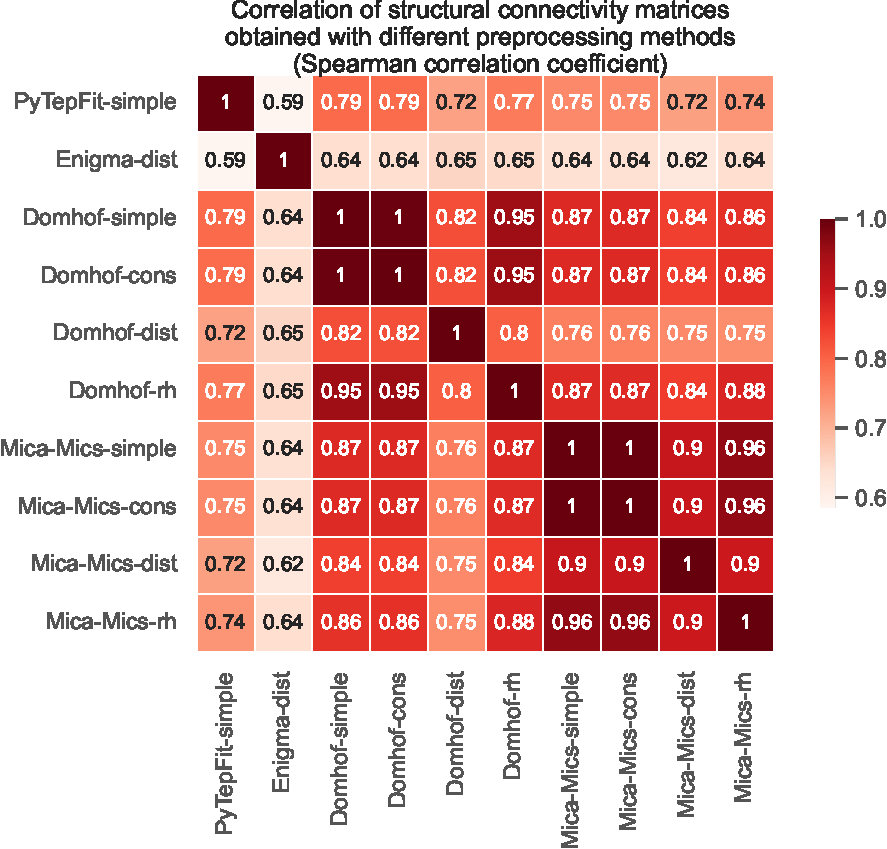
\includegraphics[width=\textwidth]{images/nootebook_generated/sc_comparison/schaefer/5/0.25/correlations_all_matrices_Spearman.pdf}
  \end{center}
  \caption[Correlations of SC matrices (Schaefer200 parcellation)]{Spearman correlations ($p<0.05$ for all results) of structural connectivity matrices with Schaefer200 parcellation. }
  \label{fig:sc_correlations}
\end{figure}


\subsection{Distribution of edge weights}

Another question is if the preprocessing method influences the distribution of edge weights. We can see in Figure~\ref{fig:edge_weights_schaefer} for the Mica-Mics dataset that the simple average is again nearly the same as consensus thresholding, and they both result in a higher number of weaker edges than Rosen and Halgren's. Rosen and Halgren's method yields proportionally a higher number of stronger edges than the other methods. The results for the Domhof dataset look similar, only the distribution for distance-dependent consensus thresholding is slightly shifted to the higher weights.

However, there is a difference if we look at different parcellations. Figure~\ref{fig:edge_weights_glasser} differs from~\ref{fig:edge_weights_schaefer} only in the parcellation, but there are much bigger differences in the edge weights distributions based on the preprocessing method. Especially there is a difference between simple average and consensus thresholding, the former having a higher number of weaker edges. Rosen and Halgren's method still gives a higher number of stronger edges than the other methods, and the effect is even more visible in this case.

The reason for the difference between the parcellations is probably caused by their different granularity. Let us remind you that Schafer200 has 200 ROIs, while Glasser 360. We use the same DW-MRI data as a basis for connectomes with both parcellations. In the case of finer parcellation, the resulting connectome may exhibit lower density. This is because if there are only a few streamlines connecting certain ROIs, further subdivisions of these regions could lead to the absence of streamlines between some pairs of ROIs in the subdivision. Therefore there are more zeros in the connectivity matrices for individual subjects for Glasser parcellation. Because of that, there is a higher number of weaker edges in the simple group average because we are averaging the zeros as well. \footnote{The effect is there even if the density is the same as for the consensus thresholding method because we are averaging only the non-zero values during the consensus thresholding connectome calculation.}

\begin{figure}[p]
\begin{subfigure}{\textwidth}
      \begin{center}
    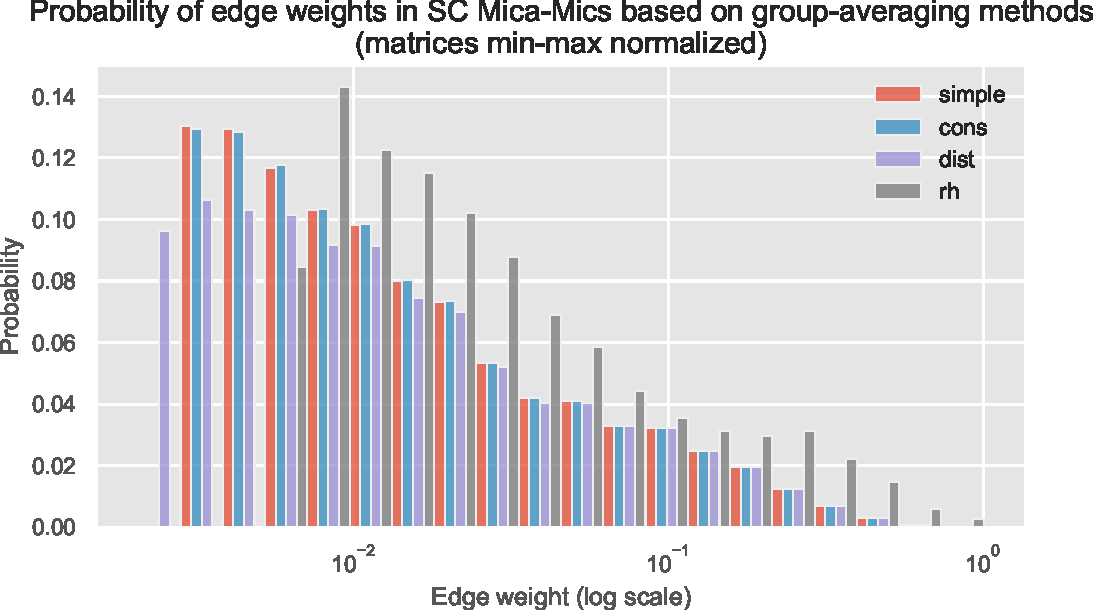
\includegraphics[width=\textwidth]{images/nootebook_generated/sc_comparison/schaefer/5/0.25/Probability_of_edge_weights_in_SC_Mica-Mics_based_on_group-averaging_methods_(matrices_min-max_normalized).pdf}
  \end{center}
  \caption{Schaefer200 parcellation}
  \label{fig:edge_weights_schaefer}
\end{subfigure}

\bigskip

\begin{subfigure}{\textwidth}
      \begin{center}
    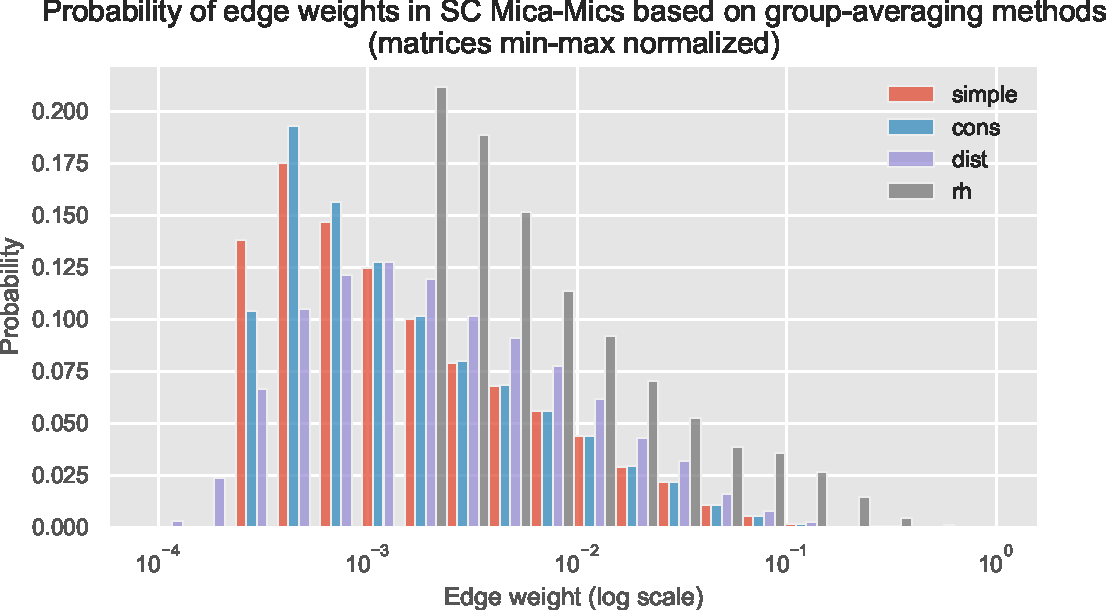
\includegraphics[width=\textwidth]{images/nootebook_generated/sc_comparison/MNI-HCP-MMP1/5/0.25/Probability_of_edge_weights_in_SC_Mica-Mics_based_on_group-averaging_methods_(matrices_min-max_normalized).pdf}
  \end{center}
  \caption{Glasser parcellation}
  \label{fig:edge_weights_glasser}
\end{subfigure}
\caption[Edge weights distribution per preprocessing method]{Edge weights distribution per preprocessing method for Mica-Mics dataset and Schaefer200 and Glasser parcellations. All matrices were min-max normalized because the weights of the rh method are not comparable with the others otherwise. The y-axis shows a probability (not count) for better comparability because the number of edges differs for the \texttt{dist} method.}
\end{figure}

\begin{figure}[p]
  \begin{center}
    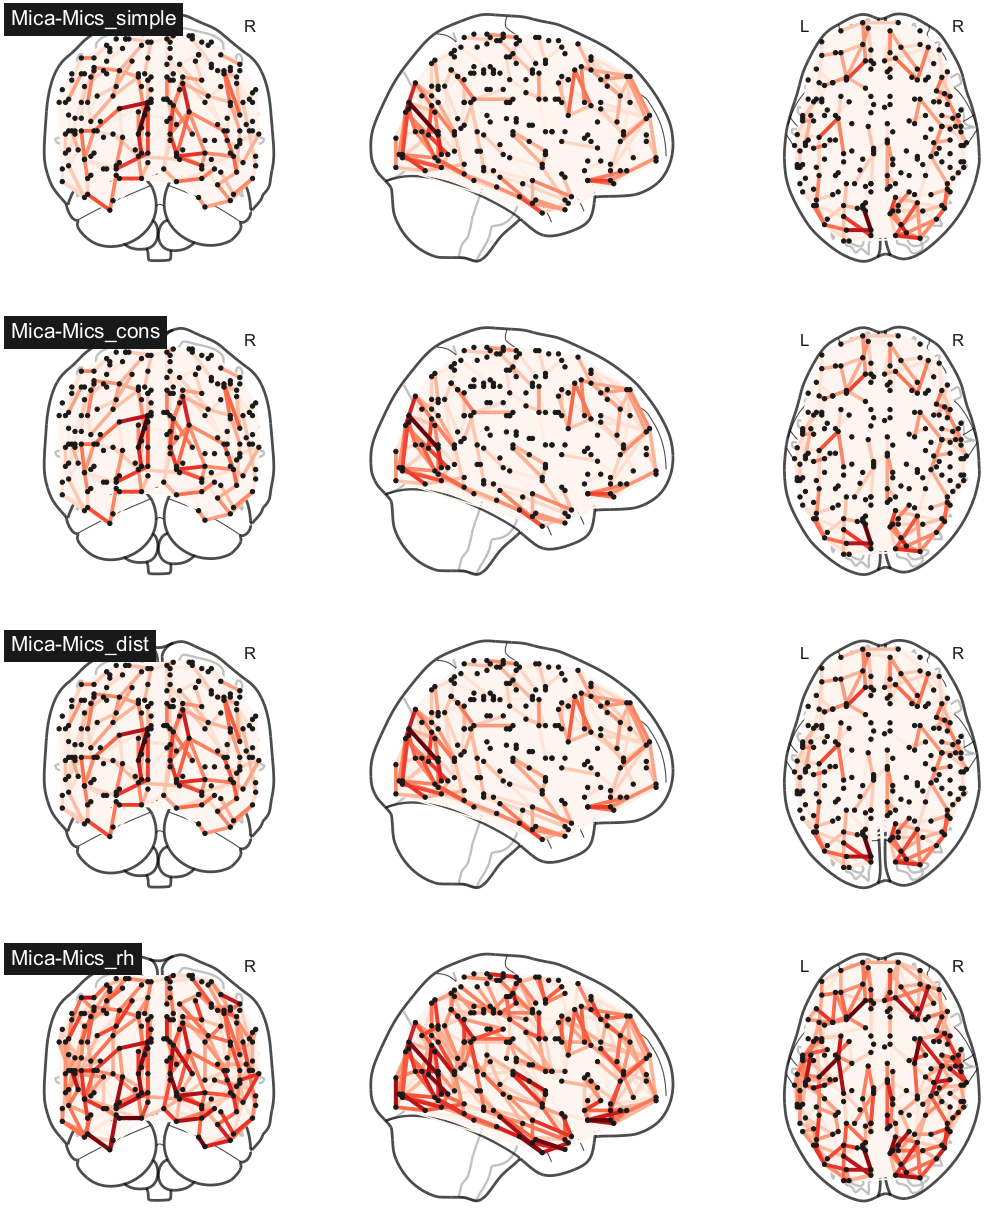
\includegraphics[width=\textwidth]{images/manually_created/mica.png}
  \end{center}
  \caption[Connectomes based on preprocessing method]{Connectomes based on group-averaging method (simple averaging, consensus thresholding, distance dependent consensus threshodling and Rosen and Halgren's method) for Schaefer200 parcellation, Mica-Mics dataset, edge weights log-transformed and min-max normalized. In a common color scale, a darker color denotes stronger edges.}
  \label{fig:connectomes_mica}
\end{figure}

\begin{figure}
\begin{center}
    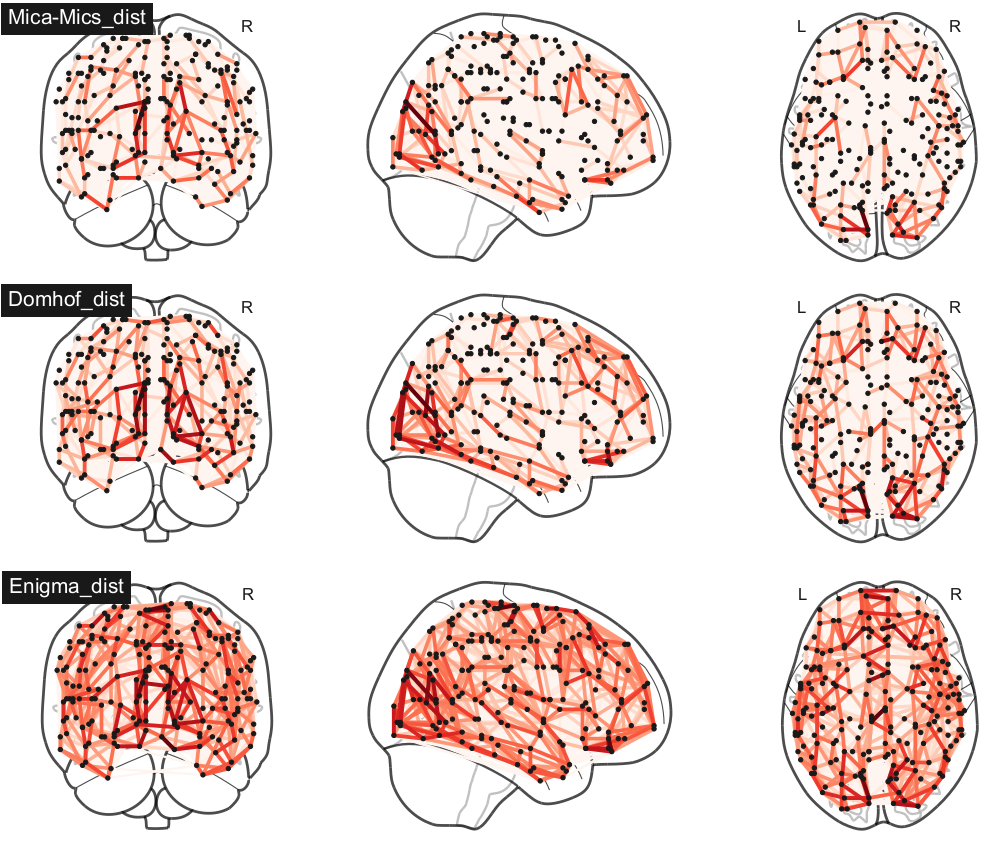
\includegraphics[width=0.9\textwidth]{images/manually_created/datasets.png}
  \end{center}
  \caption[Connectomes based on dataset]{Connectomes based on dataset (Mica-Mics, Domhof, and Enigma) for Schaefer200 parcellation, edge weights log-transformed and min-max normalized. All datasets group averaged using distance dependent consensus thresholding method. In a common color scale, a darker color denotes stronger edges.}
  \label{fig:connectomes_by_dataset}
\end{figure}

We were also curious if the distribution of edge weights in the brain differs based on the preprocessing method. Figure~\ref{fig:connectomes_mica} shows the edge weights in the brain for different preprocessing methods. It is already discussed above and shown in Figure~\ref{fig:edge_weights_schaefer} that different preprocessing methods yield different numbers of stronger edges. Besides that, Rosen and Halgren's group averaging method creates a slightly different structure than the others. However, the structure of the connectome weights differs much more based on the datasets. See Figure \ref{fig:connectomes_by_dataset}. 

\subsection{Distribution of edge lengths}

We mention in Section~\ref{sec:dist-dep} that the primary reason for the introduction of the distance-dependent thresholding method was to prevent the omission of long edges in group average connectomes. However, as shown in Figure~\ref{fig:edge_lengths}, our results do not confirm that the method fulfills this goal. Although there are slightly more longer edges for Schaefer200 parcellation, the differences in edge length distribution are really small and probably negligible. 

\begin{figure}[p]
\begin{subfigure}{\textwidth}
      \begin{center}
    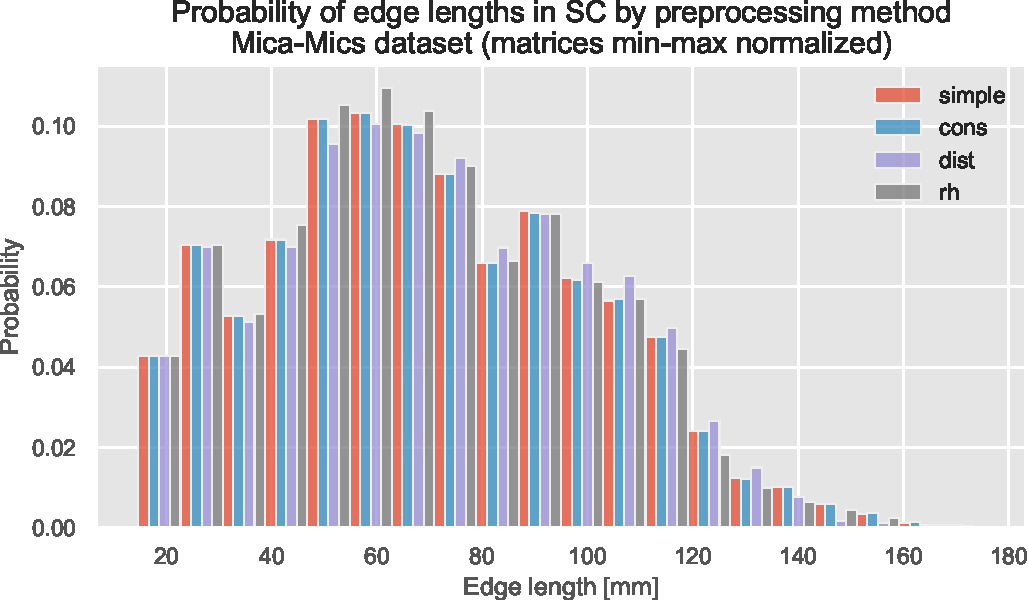
\includegraphics[width=\textwidth]{images/nootebook_generated/sc_comparison/schaefer/5/0.25/Probability_of_edge_lengths_in_SC_by_preprocessing_method_Mica-Mics_dataset_(matrices_min-max_normalized).pdf}
  \end{center}
  \caption{Schaefer200 parcellation}
  \label{fig:edge_lengths_schaefer}
\end{subfigure}

\bigskip

\begin{subfigure}{\textwidth}
      \begin{center}
    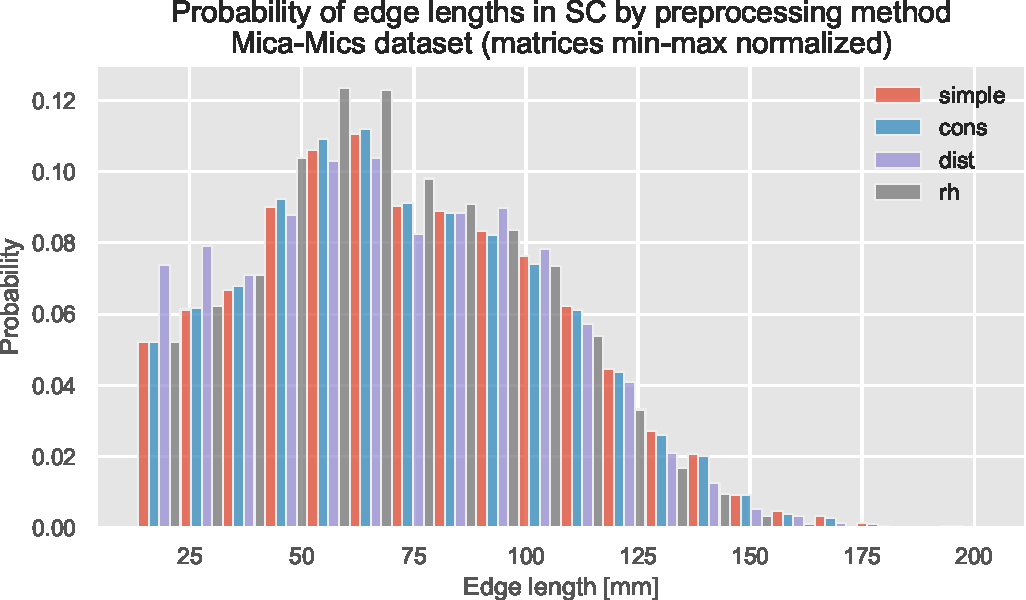
\includegraphics[width=\textwidth]{images/nootebook_generated/sc_comparison/MNI-HCP-MMP1/5/0.25/Probability_of_edge_lengths_in_SC_by_preprocessing_method_Mica-Mics_dataset_(matrices_min-max_normalized).pdf}
  \end{center}
  \caption{Glasser parcellation}
  \label{fig:edge_lengths_glasser}
\end{subfigure}
\caption[Edge lengths distribution per preprocessing method]{Edge lengths distribution per preprocessing method for Mica-Mics dataset and Schaefer200 and Glasser parcellations. The y-axis shows a probability (not count) for better comparability because the number of edges differs for the \texttt{dist} method.}
\label{fig:edge_lengths}
\end{figure}

\section{Robustness of the previous results}

Section \ref{sec:sc-robustness_ftract} already discussed the robustness of F-TRACT results to structural connectome selection. In this section, let us first discuss the results for F-TRACT obtained with Deskian-Killiany parcellation. Then, we move to TMS-EEG and look at the results with a different dataset or a group-averaging method.

\subsection{F-TRACT with Deskian-Killiany parcellation}

As mentioned in Section \ref{sec:parcellations}, the selection of parcellation can influence the results obtained later with the data. We illustrate the issue here. 

Figure  \ref{fig:ftract_alldata_long_probabilities_DK} shows that both full and partial correlations of response probability with structural connectivity and communication metrics are preserved with the change of parcellation from Glasser (360 regions) to Deskian-Killiany (68 regions), even when the results differ (for example, the highest correlation of response probability is with the structural connectivity for Deskian-Killiany, but with the shortest path efficiency for Glasser). However, Figure \ref{fig:ftract_alldata_long_amplitudes_DK} shows that for the amplitudes, there are no significant correlations when the Deskian-Killiany parcellation is used.

\begin{figure}
    \centering
    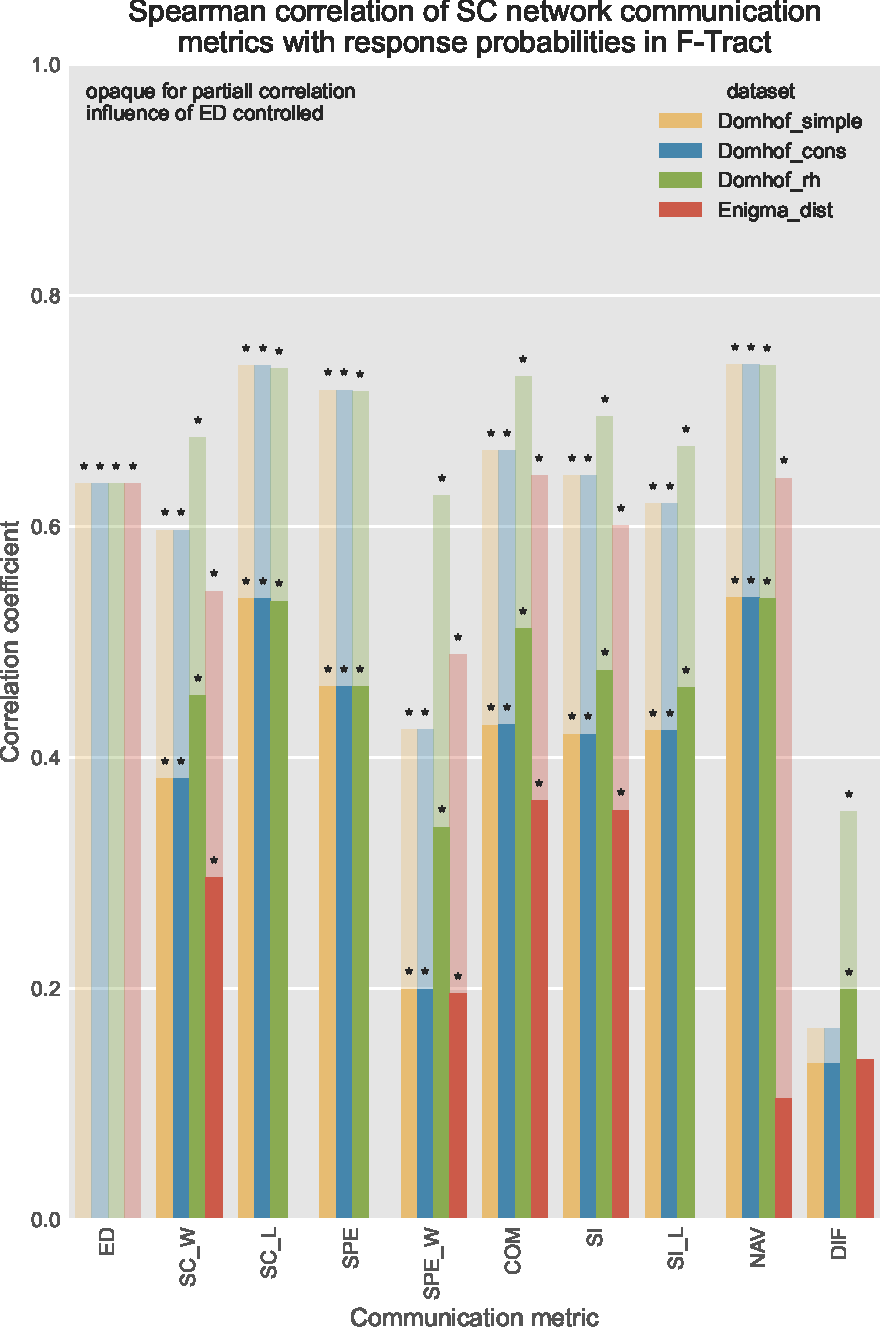
\includegraphics[width=0.93\textwidth]{images/nootebook_generated/ftract_results/DKT/5/ED0/0.25/long/Spearman_correlation_of_SC_network_communication_metrics_with_response_probabilities_in_F-Tract.pdf}
    \caption[F-TRACT probability correlations - all $SC$ matrices (DK)]{Correlations (absolute value) of response probability (200~ms response) and structural connectivity and derived communication metrics (DK parcellation). Asterisks denote a significant correlation ($p<0.05$).}
    \label{fig:ftract_alldata_long_probabilities_DK}
\end{figure}

\begin{figure}
    \centering
    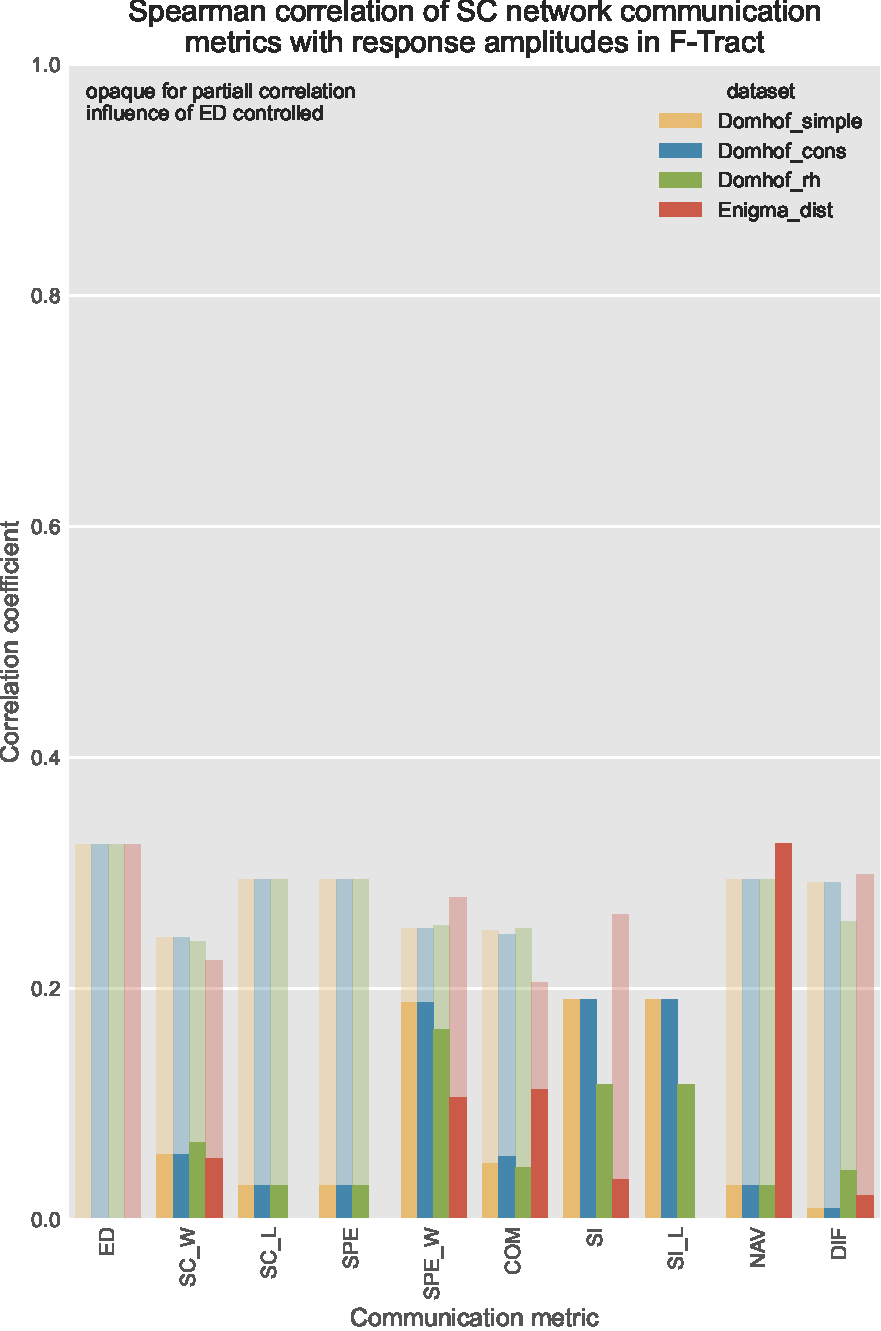
\includegraphics[width=0.93\textwidth]{images/nootebook_generated/ftract_results/DKT/5/ED0/0.25/long/Spearman_correlation_of_SC_network_communication_metrics_with_response_amplitudes_in_F-Tract.pdf}
    \caption[F-TRACT amplitude correlations - all $SC$ matrices (DK)]{Correlations (absolute value) of response amplitude (200~ms response) and structural connectivity and derived communication metrics (DK parcellation). Asterisks denote a significant correlation ($p<0.05$)}
    \label{fig:ftract_alldata_long_amplitudes_DK}
\end{figure}

\subsection{TMS-EEG with different datasets and group-averaging methods}

We tried to calculate the results from Section \ref{sec:results_pytepfit-empirical} with different datasets and group-averaging methods for the 200 ms responses as a control.  

Regarding the group-averaging method, we tried all the methods described in Section \ref{sec:group-avg}. We applied them to the Mica-Mics dataset. There are no differences in the results obtained with simple averaging, consensus thresholding, and Rosen and Halgren's method. The results obtained with distance-dependent consensus thresholding preserve the important features like high correlation of response characterized by AUC with the shortest path efficiency and the navigation efficiency (Figure \ref{fig:tms_auc_200_dist}, compare with Figure \ref{fig:tms_auc_200}), but there are differences, for example, overall lover or non-significant correlations for binarized responses (Figure \ref{fig:tms_01_200_dist}, compare with Figure \ref{fig:tms_01_200}).

\begin{figure}
    \centering
    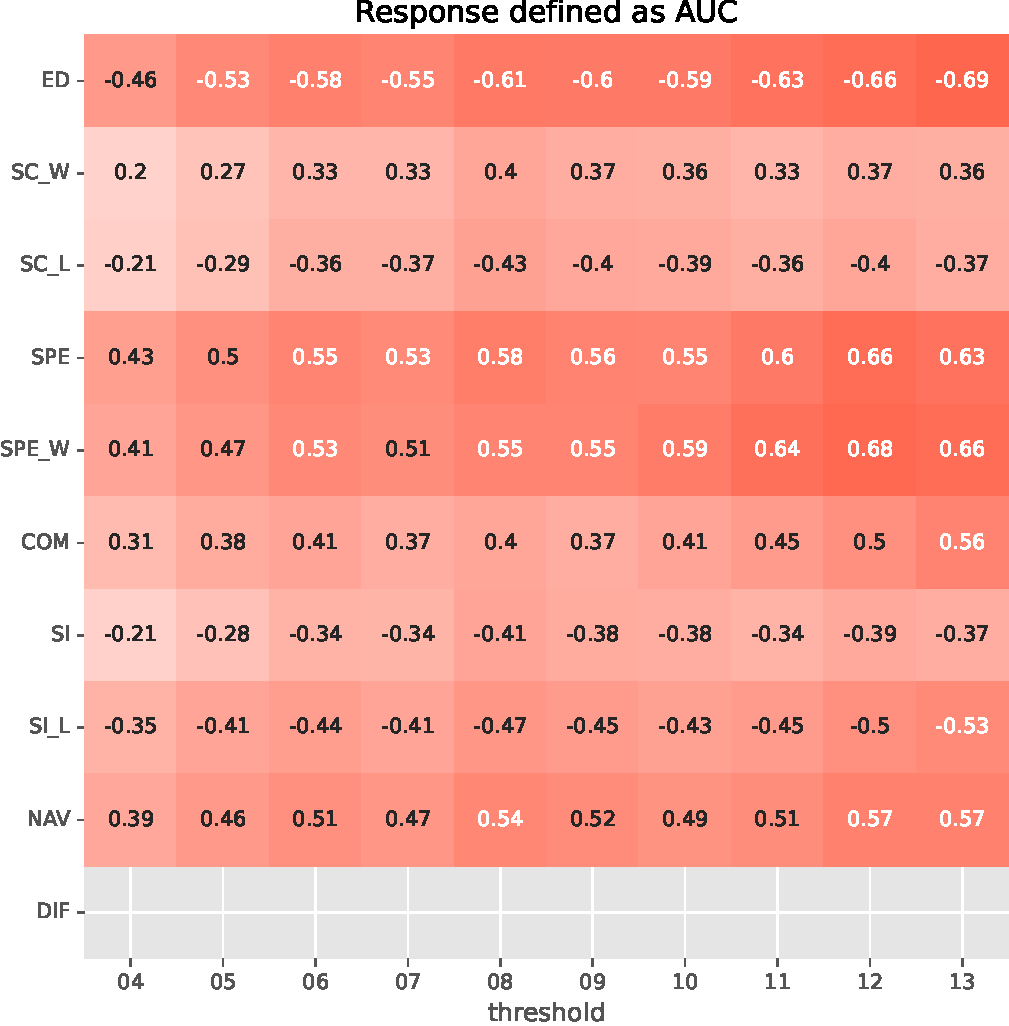
\includegraphics[width=\textwidth]{images/nootebook_generated/pytepfit_results/empirical/200/not_over_threshold_nan/Mica-Mics_dist/Response defined as AUC.pdf}
    \caption[TEPs AUC (200 ms) correlations (dist)]{Spearman correlation coefficient of AUC of empirical TEP (200 ms response) with structural connectivity and communication metrics. Darker color denoted a higher absolute value of the correlation; missing values are non-significant ($p>0.05$). Group averaging method: distance-dependent consensus thresholding.}
    \label{fig:tms_auc_200_dist}
\end{figure}

\begin{figure}
    \centering
    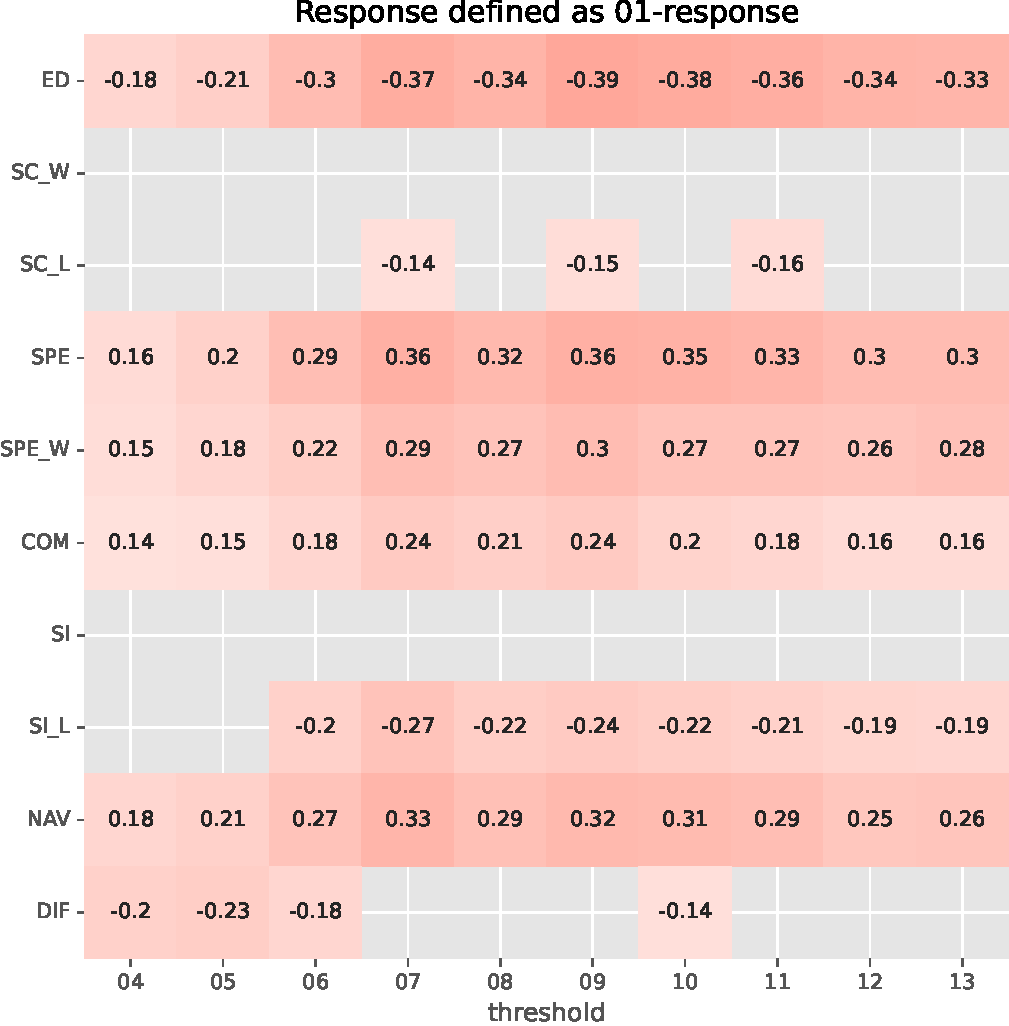
\includegraphics[width=\textwidth]{images/nootebook_generated/pytepfit_results/empirical/200/not_over_threshold_nan/Mica-Mics_dist/Response defined as 01-response.pdf}
    \caption[Binarized TEP (200 ms) correlations (dist)]{Spearman correlation coefficient of binarized empirical TEP (200 ms response) with structural connectivity and communication metrics. Darker color denoted a higher absolute value of the correlation; missing values are non-significant ($p>0.05$). Group averaging method: distance-dependent consensus thresholding.}
    \label{fig:tms_01_200_dist}
\end{figure}

Regarding the dataset, we tried Enigma \ref{sec:enigma}, Domhof \ref{sec:domhof}, and PyTepFit \ref{sec:pytepdata} datasets. The results slightly differ for all of them, but the key features discussed in Section \ref{sec:results_pytepfit-empirical} are always present: AUC and the first peak latency correlate with communication metrics, and the highest correlations are achieved for the shortest path efficiency and navigation efficiency. See Figure \ref{fig:tms_auc_200_pytep_simple} showing results for PyTepFit dataset and response characterized by AUC as an illustrative example (compare with Figure \ref{fig:tms_auc_200}).

\begin{figure}
    \centering
    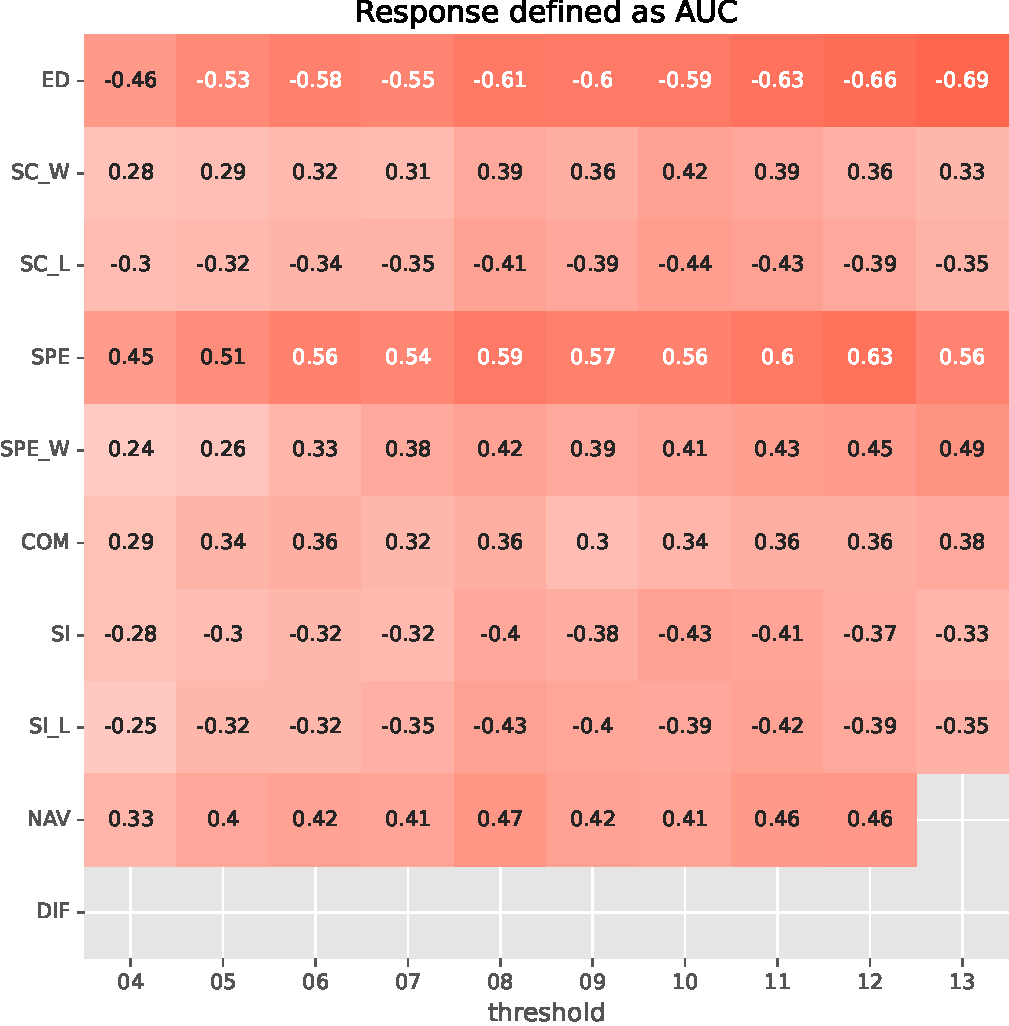
\includegraphics[width=\textwidth]{images/nootebook_generated/pytepfit_results/empirical/200/not_over_threshold_nan/PyTepFit_simple/Response defined as AUC.pdf}
    \caption[TEPs AUC (200 ms) correlations (PyTepFit)]{Spearman correlation coefficient of AUC of empirical TEP (200 ms response) with structural connectivity and communication metrics. Darker color denoted a higher absolute value of the correlation; missing values are non-significant ($p>0.05$). Group averaging method: simple averaging, dataset: PyTepFit.}
    \label{fig:tms_auc_200_pytep_simple}
\end{figure}


\section{Conclusion}

The main takeaway of this section is, that the choice of a dataset, parcellation, and preprocessing method has an impact on the resulting connectome. Consequently, the connectome has an impact on the results of subsequent analysis.

First of all, the different data sources might differ in the measurement settings, DW-MRI preprocessing, and many other aspects along the way from the human brain to the connectivity matrix. With Figure \ref{fig:sc_correlations} and Figure \ref{fig:connectomes_by_dataset} in mind, we recommend using structural connectivity matrices from different sources whenever possible because they could differ quite a lot.

The choice of parcellation is an important step as well. We aim to use graph theoretical metrics to get better insight into the brain function, and the number of nodes (not mentioning other differences of the parcellations) could have a great impact on the subsequent analysis.

Even though there are differences in the connectomes and consequently in the results, we confirmed that the observations from Chapters \ref{ch:ftract} and \ref{ch:pytepfit} are robust regarding the connectome selection.
\chapter*{Conclusion}
%% Unlike \chapter, \chapter* does not update the headings and does not
%% enter the chapter into the table of contents. If we want correct
%% headings and a table of contents entry, we must add them manually:
\markright{\textsc{Conclusion}}
\addcontentsline{toc}{chapter}{Conclusion}

The goal of this thesis was to evaluate the spatiotemporal patterns of the human brain activity evoked by direct stimulation using the methods drawn from the field of complex network analysis. Specifically, we want to look at the problem from the point of view of network communication models applied to the structural connectome graph. 

The first step on our way is the replication of the results obtained by Seguin et al. \cite{seguin_communication_2023} for iEEG measurements -- correlations of response probability and amplitude with structural connectivity matrices and network communication models. We used publicly available versions of the F-Tract dataset (50 ms and 200 ms response lengths).

We confirmed that the response probabilities and amplitudes from the F-Tract dataset correlate with the structural connectivity and network communication metrics across various settings. Among other parameters, we showed that the results are robust with respect to the structural connectivity dataset and group-averaging method, and in the case of probabilities also with respect to the brain parcellation. 

Our contribution in this part of the work is the use of structural connectivity lengths in the calculation of communication metrics. Seguin et al. \cite{seguin_communication_2023} worked only with structural connectivity weights. The lengths capture different aspect of the brain structure than weights. While the weights scale with the number of streamlines between regions,\footnote{At least in this thesis. Generally, different options exist. \cite{zhang_quantitative_2022}} the lengths capture the distance the signal has to cover between two nodes (not Euclidean distance) through the complex structure of the brain, and is proportional to the communication cost. The results in Chapter \ref{ch:ftract} show that the correlation of structural connectivity lengths with the response probability and amplitude is higher than for structural connectivity weights, but the lengths still explain less variability in the response probability than the network metrics based on communication models.

We also examined the correlations in the case of single ROI stimulation. Considering a single stimulated region (corresponding to one row in the F-Tract matrix of probabilities) builds a connection between the F-Tract dataset consisting of many pairs of stimulated and recording regions and our TMS-EEG data with a single stimulation target. However, this step is limited by the fact that the F-Tract dataset does not contain the probabilities of activation for all pairs of stimulated and target regions. We faced this limitation during the search for the region in the Glasser parcellation used in the F-Tract corresponding to the region stimulated in our TMS-EEG data. We overcame this obstacle by choosing a region that was the second-best fit according to the Dice score, but its row in the F-Tract matrix contains more data. This compromise may cause some inaccuracies in the results.

Keeping in mind the limitations, the results obtained for F-Tract serve as a basis for evaluating the extent to which these observations can be replicated in noninvasive stimulation and recordings. 

Moving to the TMS-EEG data, we proposed and tested several characteristics of the response, all of them including a threshold to filter out baseline activity. Binarized response, AUC, and the first peak latency show significant correlations with the network communication metrics across various thresholds for empirical TMS-EEG data. On the other hand, the highest peak as a response characteristic does not show significant correlations with communication metrics, which is in contrast with amplitudes in the results for the F-Tract dataset. One of the possible reasons for this mismatch might lie in the limitations of the source reconstruction applied to the EEG scalp signals, which is necessary to obtain the estimate of activity in the space of the brain. Because of that, it does not capture the peak heights well.

Besides the empirical TMS-EEG data, we repeated the analysis for simulated data by Momi et al. \cite{momi_tms-evoked_2023}. There is a link between the results in response characterization by first peak latency; it correlates well with communication metrics for both empirical and simulated data. On the other hand, the area under the curve, which shows high correlations for empirical data, is much worse for simulated data. A possible reason for this is that the model used for data simulation models the first peak timing quite well because it is a simple characteristic but fails to model the overall complexity of the response captured by AUC in empirical data. This might be a suggestion for improvement of the model for artificial TMS-EEG data generation.

Comparing the results for TMS-EEG empirical data with F-Tract, we see that the correlations with the communication models and the structural connectomes are overall lower. That is not a surprise because of the indirect nature of TMS-EEG. More importantly, there are no partial correlations for TMS evoked response with structural connectivity and communication models when we control the influence of Euclidean distance, no matter how it is characterized. This is related to the fact that the correlation of TMS-evoked response is always higher with the Euclidean distance than with the communication metrics. In conclusion, although the TMS-evoked response correlates with the network communication metrics, Euclidean distance influences its character greatly.

In order to get better insight into the difference between response probability and its characterization in TMS-EEG, which may be the reason for the difference in correlations with communication metrics, we compare the response probabilities and characteristics with each other. Direct comparison is impossible with the publicly available data because the datasets do not share a common parcellation. Because of that, we used the Dice score for mapping from Schaefer 200 (TMS-EEG) to Glasser (F-Tract) parcellation. It resulted in a Spearman correlation coefficient $r\approx0.5$ between the response probabilities and AUC or first peak latency. That suggests that there is a relationship between the probability and other response characteristics and its investigation may be a subject of further research. We also confirmed that the mapping is reasonable by checking the correlation of Euclidean distances in the two parcellations. However, we used a greedy approach, assigning the Schaefer ROI with the highest Dice score to each Glasser ROI, which left some Schaefer ROIs unused. 

Our experiments are limited by several aspects of the used TMS-EEG data. First of all, we have only one dataset with only one stimulation target. We searched for other publicly available datasets with stimulation at the same site or elsewhere, but our search was unsuccessful. We found a paper by Fecchio et al. \cite{fecchio_spectral_2017} providing TMS-EEG data for the primary motor cortex and other cortical sites, but unfortunately, the data are not source-reconstructed. EEG source reconstruction is beyond the scope of this thesis, but it might be a further direction of research.

Another limitation comes with the fact that the TMS-EEG data are group-averaged for the purposes of this thesis. It would be interesting to do the analysis on a subject level because group averaging of the time series could veil some aspects of the TMS-evoked response.

We performed a robustness analysis for all the results. We confirmed that the correlations are not dependent on specific structural connectivity datasets. Regarding the group averaging method, it seems to us that Rosen and Halgren's method is the best choice in this case. However, the differences are small and further analysis would be needed to confirm that. We also tried to use different parcellations for the F-Tract dataset, which shows the importance of parcellation selection.

And what about the question raised in Chapter \ref{ch:networks}, asking if the centralized models explain communication within the brain better than decentralized ones? Our results show the highest correlation of the response with the most common centralized communication models, shortest path efficiency, for both F-Tract and TMS-EEG data. It is followed by navigation efficiency, which is a centralized metric as well. However, the success of navigation efficiency should be interpreted carefully, as it utilizes Euclidean distance, which itself correlates with the responses very well.

\section*{Future work}

To conclude the work, let us summarize possible directions for future work. The first natural next step is to compare the TMS and F-Tract data for other ROIs while harmonizing the parcellation used for the source reconstruction with F-Tract, which would allow direct comparison of the results.

Another direction would be a detailed analysis of the late response complexity discrepancies of the empirical and simulated TMS-EEG data. Such analysis would be beneficial for further improvement of the model generating the synthetic data.

Last but not least, it would be interesting to leverage the advantage of the noninvasive nature of TMS-EEG to study inter-subject variability of the TMS-evoked responses, which is not possible for the intracranial data in F-Tract.

\printbibliography

\appendix %% Start the appendices.

\chapter{Implementation}

\TODO[že jsou k tomu notebooky a kde]

\end{document}
